\documentclass[nofilelist]{cslthse-msc}
% to show a list of used packages at the end of the document, delete the nofilelist option
%\documentclass{cslthse-msc} 
\usepackage[utf8]{inputenc}
\usepackage[english]{babel}
\usepackage{amsmath}
%\usepackage{amsfonts}
%%\usepackage{amssymb}
\usepackage{amsthm}
%\usepackage{makeidx}
\usepackage{graphicx}
\usepackage[titletoc, header, page]{appendix}
\usepackage{transparent}
\usepackage{svg}
\usepackage[numbers]{natbib}
\usepackage{adjustbox}
\usepackage{amssymb}

\usepackage{array}  
\usepackage{xcolor}
\usepackage{subfig}
\usepackage{changepage}
\usepackage{amsmath}
\usepackage{pifont}
\usepackage{times}
\usepackage{fancyhdr,graphicx,amsmath,amssymb}
\usepackage[ruled,vlined]{algorithm2e}
%\include{pythonlisting}



% Use hyperlinks for citations?
\usepackage{hyperref}

\usepackage{listings}
\usepackage{xcolor}
\usepackage{todonotes}
\usepackage{float}
\usepackage{changepage}
\usepackage{booktabs}
\usepackage{multirow}

\colorlet{punct}{red!60!black}
\definecolor{background}{HTML}{EEEEEE}
\definecolor{delim}{RGB}{20,105,176}
\colorlet{numb}{magenta!60!black}

\lstdefinelanguage{json}{
    basicstyle=\normalfont\ttfamily,
    %numbers=left,
    numberstyle=\scriptsize,
    %stepnumber=1,
    numbersep=8pt,
    showstringspaces=false,
    breaklines=true,
    frame=lines,
    %backgroundcolor=\color{background},
    literate=
     *{0}{{{\color{numb}0}}}{1}
      {1}{{{\color{numb}1}}}{1}
      {2}{{{\color{numb}2}}}{1}
      {3}{{{\color{numb}3}}}{1}
      {4}{{{\color{numb}4}}}{1}
      {5}{{{\color{numb}5}}}{1}
      {6}{{{\color{numb}6}}}{1}
      {7}{{{\color{numb}7}}}{1}
      {8}{{{\color{numb}8}}}{1}
      {9}{{{\color{numb}9}}}{1}
      {:}{{{\color{punct}{:}}}}{1}
      {,}{{{\color{punct}{,}}}}{1}
      {\{}{{{\color{delim}{\{}}}}{1}
      {\}}{{{\color{delim}{\}}}}}{1}
      {[}{{{\color{delim}{[}}}}{1}
      {]}{{{\color{delim}{]}}}}{1},
}

% used to display the used files at the end. Select nofilelist as a package option to disable this
\listfiles % initialize

%\geometry{showframe}
%better like this?
%\student{Flavius Gruian}{Flavius.Gruian@cs.lth.se}
\students{Simon Erlandsson}{si5417er-s@student.lu.se}{Leo Westerberg}{le8037we-s@student.lu.se}

\thesisnumber{LU-CS-EX: 2023-79} % Magic Number! Do not change unless Birger Swahn asks you to do so!
% default is Master. Uncomment the following for "kandidatarbete"/Bachelor's thesis
%\thesistype{Bachelor}{Kandidatarbete}

%\title{Formatting a Master's Thesis}
\title{Compression Algorithms for Geometries Supporting Operations}
\svensktitel{Komprimeringsalgoritmer för geometrier med stöd för operationer}

%\onelinetitle
%\twolinestitle
\threelinestitle
%\fourlinestitle

%\subtitle{A {\LaTeX} class}
\company{AFRY AB}
\supervisors{Hampus Londögård, \href{mailto:hampus.londogard@afry.com}{\texttt{hampus.londogard@afry.com}}}{Jonas Skeppstedt, \href{mailto:jonas.skeppstedt@cs.lth.se}{\texttt{jonas.skeppstedt@cs.lth.se}}}
%\supervisor{John Deer, \href{mailto:jdeer@company.com}{\texttt{jdeer@company.com}}}
\examiner{Per Andersson, \href{mailto:per.andersson@cs.lth.se}{\texttt{per.andersson@cs.lth.se}}}

%\date{\today}
\date{July 14, 2023}
%\date{January 16, 2015}

\acknowledgements{
A massive thank you goes out to everyone who has played a part in this thesis.
\\\\
We want to thank Björn Pedersen, Hampus Londögård, and Per Svensson for their invaluable feedback and guidance throughout the thesis, along with welcoming and integrating us into the data analytics team at AFRY. Your optimism and genuine excitement for problem-solving have been truly motivating.
\\\\
Thanks to Patrick Cording and Martin Lindberg for their shared expertise in compression algorithms and the maps-domain. We also appreciate their insights into potential career paths and for sharing their experiences when working with technology and big data.
\\\\
Additionally, we would like to thank Per Andersson and Jonas Skeppstedt for their oversight of the academic aspects of the thesis and for serving as our link to Lund University.
\\\\
Lastly, we want to thank all colleagues, including Dan Svenonius and Tim Jangenfeldt, for their great company throughout the thesis. 


% If you want to thank people, do it here, on a separate right-hand page. Both the U.S. \textit{acknowledgments} and the British \textit{acknowledgements} spellings are acceptable.

% We would like to thank Lennart Andersson for his feedback on this template.

% We would also like thank Camilla Lekebjer for her contribution on this template, as well as Magnus Hultin for his popular science summary class and example document.

% Thanks also go to the following (former) students for helping with feedback and suggestions on this template: Mikael Persson, Christoffer Lundgren, Mahmoud Nasser.
}

\theabstract{
Maps-services providers use vast amounts of geometric data to represent the structures of the world. With increasing amounts of data, the required storage and transmission capacities increase.

Existing compression algorithms can reduce the size of the data at the cost of operability. Namely, any operation requires the entire compressed geometry to be unpacked, resulting in an overhead that may be longer than the operation itself. When performing enormous amounts of operations, such as when validating map fragments, the overhead can be significant.

This thesis aims to create a compression format that reduces the data size of geometries, beyond general-purpose algorithms, while maintaining speed on some specific operations.

The implemented format utilizes delta encoding, a maps-specific coordinate structure, and entropy encoding to reduce the size. In addition, the coordinates are divided into independent blocks, allowing for partial decompression. Partial decompression can be used to avoid decoding irrelevant sections of the geometries. For example, when calculating the \emph{intersection} between two shapes, only the overlapping blocks can contain an intersection point.

{\color{black}During testing, the implementation achieved an average compression factor of 2.56, compared to the WKB standard format. Additionally, with partial decompression enabled, it achieved an average speedup of 3.6 times faster execution when calculating the \textit{intersection} over large geometries, compared to full decompression.} Partial decompression of geometries is largely unexplored in academia, but the results of the thesis indicate that the area may be of interest to investigate further.

% This document describes the Master's Thesis format for the theses carried out at 
% the Department of Computer Science, Lund University. 

% Your abstract should capture, in English, the whole thesis with focus on the problem and solution in 150 words. It should be placed on a separate right-hand page, with an additional \textit{1cm} margin on both left and right. Avoid acronyms, footnotes, and references in the abstract if possible.

% Leave a \textit{2cm} vertical space after the abstract and provide a few keywords relevant for your report. Use five to six words, of which at most two should be from the title.
}

 \keywords{geometry compression, maps, partial decompression, compressed computation}%MSc, BSc, template, report, style, structure}

%% Only used to display font sizes
\makeatletter
\newcommand\thefontsize[1]{{#1 \f@size pt\par}}
\makeatother
%%%%%%%%%%

\newcommand{\starsection}[1]{%
  \refstepcounter{section}%
  \section*{\thesection*\hspace{1ex}#1}%
  \addcontentsline{toc}{section}{\protect\numberline{\thesection*}#1}%
}

\newcommand{\starsubsection}[1]{%
  \refstepcounter{subsection}%
  \subsection*{\thesubsection*\hspace{1ex}#1}%
  \addcontentsline{toc}{subsection}{\protect\numberline{\thesubsection*}#1}%
}

\begin{document}
\renewcommand{\bibname}{References}

    \makefrontmatter

\chapter[Introduction]{Introduction}
\section{Background}

% ·\todo{skriv om att är kombo av impl. och påkommen teori}

Geometric data is a powerful tool for describing spatial relationships between physical objects. In online maps services, geometries are frequently used to represent various structures on the map, such as roads and buildings. By modeling an area as geometric objects, spatial relationships can be inferred directly or explicitly stated, enabling analysis and querying of the data. However, due to the inherently extensive information size for creating a detailed map, minimizing the needed data storage and transmission capacity while maintaining optimal performance is of great interest to map service providers.

Compression algorithms can reduce the size of modeled maps by eliminating redundancies in the data. However, conventional algorithms transform the data to an inoperable state, requiring the data to be decompressed before it can be operated on. Additionally, operations that involve modifications to the map require the compressed data to be recompressed to maintain a coherent representation. Since these steps can be time-consuming, integrated operability of compressed geometries could reduce the overhead of needing to fully decompress the data while still allowing for a reduction in size by utilizing compression methods. This way, a balance between reducing storage space and efficient operations can be established.

Furthermore, general-purpose compression algorithms are not tailored to operate on maps data. Therefore, it may be possible to increase the size reduction beyond common compression algorithms by exploiting the maps domain and combining existing compression schemes.
\\\\
AFRY is working on enhancing maps services and would like to investigate potential improvements in the geometry pipeline with regard to space and time efficiency. For map applications, being able to perform operations, such as determining intersections between objects in the map, allows for further validation checks and relationships. For instance, determining where a house polygon intersects with a lake polygon in order to classify the area.

\section{Problem Definition}
Considering the background, the following research questions have been established:
\begin{description}
    \item[Q1:] Is it possible to perform operations on compressed geometric data without decompressing the entire geometries?
    \item[Q2:] How can domain-specific constraints and structures, in the context of maps, be exploited to improve the performance of operations and geometry compression?
\end{description}
This also includes being able to decompress the data back to its original form without loss after compression has been applied.
 \\\\
Modern compression algorithms are usually improvements or combinations of prior methods. The investigation will similarly modify different compression schemes to embody unary operations on single geometrical objects, as well as binary operations where two geometrical objects interact. 
\\\\
The project is anticipated to make a scientific contribution by exploring how existing compression algorithms can be adapted to a niche datatype, while preserving or improving operation performance. Research regarding operating on compressed geometric data is currently limited.

\label{scopeLimit}
\section{Scope \& Limitations}
The project's domain will be maps data where geometrical forms such as points, polylines, and polygons are used to describe different objects. The investigation will focus on the more frequent operations made on map data and be limited to two-dimensional geometries. In order to limit the scope, three operations: intersection, bounding box, and adding vertices to a shape, are primarily optimized in the thesis.
\\\\
Furthermore, existing compression schemes will be used, and the goal of the thesis is not to invent a principally new compression algorithm but to combine existing compression schemes, data structures, and algorithms to improve operational efficiency and compression efficiency in terms of size in the spatial data domain.
\\\\
The algorithm implementations in the thesis are written in Python. The reason for the choice is to enable fast iterations and high productivity in a project which requires much exploration of different implementation designs. Due to Python being an interpreted language, lacking compilation and extensive optimization, Python is not an ideal language in terms of speed. In order to counter this, a comparison baseline is written in Python, and the relative difference in performance between the implementations is used as a means of evaluation. The resulting compression size is language-independent and thus unaffected by Python's limitations.

\section{Related Work}
There are little to no earlier attempts in the investigation of doing operations on compressed geometry data. However, compression algorithms are still at the foundation of this thesis, and the structure of creating a compression format, and supporting operations, rely heavily on previous work and ideas.

\subsubsection{Spatial Parquet: A Column File Format for Geospatial Data Lakes}
In a paper by \citet{spatialparquet} in 2022, the column-based storage format Parquet is extended with efficient support for spatial data. In column-based storage, homogeneous values are grouped together, making it possible to use their redundancies to create efficient storage. Delta encoding is a well-known method for storing differences between values rather than the complete values. However, for spatial data, with coordinates consisting of floating-points, a small floating-point value does not necessarily mean that fewer bits are needed. To tackle this, the paper suggests floating-point delta encoding, which interprets the underlying structure of floating-point values as integers and calculates the delta. The paper also proposes a method to partition the column values into independent data sections, allowing for separate compression of the units \cite{spatialparquet}. 

Floating-point delta encoding and partitioning of compressed data are two concepts that are useful for the thesis. The prior allows for a compact representation of a sequence of coordinates, while the latter enables indexing and fractional compression opportunities by dividing regions within geometries into independent chunks.

\subsubsection{Fast and Efficient Compression of Floating-Point Data}

\citet{fpzip} proposes a state-of-the-art lossless compression scheme targeted at floating-point data concerning bottlenecks where the growth of the dataset exceeds the available I/O bandwidth. The essence of the algorithm is to store the residuals between the actual floating-point values and their corresponding predicted value, where the prediction is accomplished using a subset of previously encoded data. Similarly to \citet{spatialparquet}, the bit sequence of the floating-point value and the prediction are interpreted as sign-magnitude binary integers before calculating their difference. The reason is a possible loss of information due to underflow when using floating-point subtraction. Furthermore, when the residuals have been computed, they are subject to entropy range encoding, a variant of arithmetic encoding leading to even higher compression ratios.

Besides the concept of using residuals between actual values and predicted ones, this paper gives insight into how multiple compression methods can be combined into a longer pipeline. Also, noticing similarities between different sources gives an understanding of what is considered good practice in the industry.

\subsubsection{RasterZip: Compressing Network Monitoring Data with Support for Partial Decompression}

RasterZIP, proposed by \citet{localDecomp}, is a lossless encoding scheme for network traffic data with support for partial compression and decompression. The format exploits patterns in traffic data, such as the common prefixes in IP addresses, to compress beyond the limits of general-purpose algorithms. By using partial compression, RasterZIP has the ability to compress more than half a million traffic records per second, while only targeting compression and decompression on tiny fractions of the dataset.

When integrating operations into a compression scheme, partial decompression is an excellent method for only unfolding relevant dataset fractions for the operation. The concept of partial decompression is at the core of many of the operation implementations in this thesis.

\subsubsection{A Simple Algorithm for Boolean Operations on Polygons}
Polygon clipping is a geometrical operation that constrains a polygon to fit within a defined region. Specifically, one polygon defines the area to be clipped, while another determines the clipping boundaries. Algorithms for boolean operations on polygons, with their basis in polygon clipping, are typically accompanied by geometrical constraints. For example, disallowing internal holes within the polygons or requiring the clipping boundaries to be either convex or rectangular. \citet{polygonclipping} proposes an efficient way of performing boolean operations on polygons, even in degenerate cases. The foundation of the algorithm is to subdivide the edges at their intersection points and categorize the edges as lying either inside or outside the other polygon. Depending on the boolean operation, edges with similar inside-outside statuses are selected and interconnected. The algorithm uses many efficient techniques, such as an extended version of the sweep lines algorithm by Bentley and Ottmann \cite{sweeplines} for finding intersection points in $\mathcal{O}((n + k) \log (n))$ time, where $n$ is the number of line segments and $k$ is the number of crossings.

This paper helped to understand how intersections between different geometries can be calculated in more advanced cases without constraints. Even though the algorithm this thesis proposes for intersection only uses a subset of all the edges in the geometry, many of the ideas are based on \citet{polygonclipping}.

\section{Disposition}

\begin{description}
    \item [Introduction] In the outline, the section describes the background and context of the thesis. Subsequently, the research questions are stated together with the scope and limitations. Lastly, related work with closely connected research papers and contribution statements are presented.
    
 
    \item [Theoretical Background] Provides the necessary theoretical background on spatial data and compression to understand the subsequent parts of the thesis.
    
    \item [Methodology] Introduces the methodology used to answer the research questions and conduct a robust investigation.
    
    \item [Algorithm Implementations] Describes the implementation phase of the thesis, with details about the created compression scheme and how support for several operations was integrated.
    
   
    \item [Results] Presents and reasons about the various results made from the previous sections.

    
    \item [Discussion] Consists of a further evaluation of the obtained results. Additionally, the research questions are explicitly answered, followed by potential future work.
\end{description}

% \todo{}

\section{Contribution Statement}
The work for this thesis, including writing the report, research, planning, implementing algorithms, and brainstorming ideas, was completed in full cooperation between the authors. Most of the implementations were completed in office, with frequent discussions, pair programming, and switching between individual tasks. When not working physically together, all individual work was processed and discussed internally. This also includes the study of literature, where the material was thoroughly discussed to provide both authors with the same background knowledge. In conclusion, both authors contributed equally and played crucial roles in the finalization of this thesis.
\\\\
The original work of the thesis includes the code available in Appendix, along with most of the ideas and structures proposed in Chapter \ref{sec:chapterimplementation}. For example, the proposed algorithms for adding vertices and calculating intersection through chunk-based local decompression are original ideas. Furthermore, integrating and evaluating existing compression techniques into a format that supports local decompression combined with the exploitation of the maps domain to further reduce the data size, such as by utilizing integer decomposed coordinates, is original work of the authors.

\chapter{Theoretical Background}

This section introduces existing algorithms, data structures, and metrics relevant to the thesis. First, various types of geometries and common encoding schemes for singular geometries are introduced. Next, descriptions of some compression algorithms in different categories are provided, followed by in-depth details on floating-point representations and delta encoding. Finally, additional compression schemes, some evaluation metrics, and an introduction to spatial indexing are presented. The sections marked with an asterisk (*) are not directly referenced in the thesis and are therefore optional, but may provide a deeper knowledge of existing compression algorithms and understanding of the design choices made in Chapter \ref{sec:chapterimplementation}.

% \todo{\textbf{*}}

\section{Geometries \& Encoding}
\subsection{Geometry Types}
%https://en.wikipedia.org/wiki/Well-known_text_representation_of_geometry
%+ Spatial Parquet paper
\begin{figure}[htbp]
    \centering
    \includesvg[width=8.8cm]{images/geom_types.svg}
    \caption{Descriptions of different geometry types.}
    \label{img:geom_type}
\end{figure}
Four primary types of geometries are commonly used in geometry frameworks: Point, LineString, Polygon, and GeometryCollection. Multipart alternatives consisting of several primitive geometries, such as MultiLineString, are also often included \cite{spatialparquet}.

\begin{description}
    \item[Point] is represented by a pair of the $(x, y)$ coordinates in the plane.
\item[LineString] also referred to as Polyline, is a sequence of points $\langle(x_1,y_1), ..., (x_n,y_n)\rangle$, where two adjacent points in the sequence form a straight line segment.

\item[Polygon] is similar to LineString, but the last point is always equal to the first point, such that the line segments form a closed path. As seen in Figure \ref{img:geom_type}, a polygon may include additional closed paths within the shell, forming holes in the shape. The paths, called \emph{rings}, are represented by a sequence of closed LineStrings, where the first ring is the shell.

\item[GeometryCollection] is a set of geometries, where each geometry can be of any type supported by the framework, including another GeometryCollection. The collections can therefore be used to categorize shapes into a tree-like structure.
\end{description}

Furthermore, as seen in Figure \ref{img:geom_type}, shapes may consist of multiple combined geometries of the same type, namely MultiPoint, MultiLineString, and MultiPolygon. The approach for storing those geometries is similar to GeometryCollection, but without recursive types \cite{spatialparquet}.


\subsection{Geometry Encoding}
% \todo{side by side}

\begin{figure}[htbp]
    \centering
\begin{lstlisting}[language=json,firstnumber=1,basicstyle=\footnotesize\ttfamily]
{ "type": "FeatureCollection",
  "features": [
  {   "type": "Feature",
      "geometry": {
        "type": "Point"
        "coordinates": [55.2517, 12.6543]},
      "properties": { "map_type": "POI" }
}]}
\end{lstlisting}
\caption{GeoJSON format representing a point.}
    \label{fig:geojson}
\end{figure}



Three commonly used data formats for storing geometries are \textit{well-known text} (WKT), \textit{well-known binary} (WKB), and \textit{GeoJSON}. GeoJSON stores geometry information in a JavaScript Object file, with the geometries starting in a collection called \textit{FeatureCollection}, as shown in Figure \ref{fig:geojson}. For each feature, the type of geometry is indicated in the \textit{type} field, along with additional attributes such as \textit{coordinates} \cite{GeoJSON}.

\begin{figure}[htbp]
\begin{lstlisting}[language=json,firstnumber=1, basicstyle=\footnotesize\ttfamily]
GEOMETRYCOLLECTION (POINT(1.25 3.47), LINESTRING(8.2 2.3, 5.5 1.8))
POINT (2.2 88.1)
POLYGON ((10 60, 70 30, 20 20, 10 20, -30 -10))
\end{lstlisting}    
\caption{Well-known text (WKT) format representing a GeometryCollection, LineString, Point, and Polygon.}
    \label{fig:wkt}
\end{figure}

The more straightforward WKT format, as seen in the example in Figure \ref{fig:wkt}, represents each geometry in plain text with the geometry type followed by an ordered sequence of coordinates. The ordered sequence of coordinates can be divided into groups, notated by encapsulating parenthesis, to maintain the geometry structures. For instance, in a polygon with holes, each ring's coordinates are held within separate parenthesis \cite{WKT}.

Well-known binary is information-wise equivalent to well-known text, but it is represented in a more compact binary form and is better served for data transportation \cite{WKB}. Even though these three geometry representations vary in size, they are all considered to be in uncompressed form.





%https://en.wikipedia.org/wiki/Well-known_text_representation_of_geometry
%https://en.wikipedia.org/wiki/GeoJSON#Example
%https://en.wikipedia.org/wiki/OpenStreetMap
%https://medium.com/@thegeospatialnews/how-are-google-maps-different-from-openstreetmap-bc65f704cdab

\section{Introduction to Compression}
The following section explains some of the principle concepts used in compression, while Table \ref{table:compalgos} provides a brief overview of some of the most commonly used compression schemes. 

%https://geekyhumans.com/de/most-popular-data-compression-algorithms/
%https://en.wikipedia.org/wiki/Data_compression
%https://ethw.org/History_of_Lossless_Data_Compression_Algorithms
%https://www.researchgate.net/publication/317599235_Modern_Lossless_Compression_Techniques_Review_Comparison_and_Analysis

% \todo{NOTE: Jag har gjort lite ändringar i tabellen så kopiera in den om du gör ändringar så det inte skrivs över}



\subsection{Lossy and Lossless Methods}
Compression algorithms can be divided into two categories; lossy and lossless methods. Lossless methods allow for the compressed data to be fully restored by decompression. In contrast, lossy methods allow some data to be permanently lost to achieve a higher compression ratio. 

Lossless methods are usually purely algorithmic, focusing on structuring the data in a clever way such that the algorithm can be performed backwards to restore the data back to its original form.

On the other hand, lossy methods are often statistically based, where an approximative model is created, which can be used to predict the original data based on features and context. For example, neighboring pixels in an image are likely to be similar in color. By accepting some, often indistinguishable, loss, a higher compression ratio can be achieved since small variations in the data can be ignored. Furthermore, domain-specific optimizations, such as removing frequencies that are out of the human hearing range and reducing the color palette in images, are considered lossy methods. 

Some areas which use lossless methods are scientific research data, general file compression algorithms (ZIP, RAW, FLAC), and databases. Lossy compression is used in, for example, 
images and video, voice communication, and audio files (MP3) \cite{lossyAndLossless}.

\begin{table}[H]
{\setlength{\extrarowheight}{9pt}%

\resizebox{\textwidth}{!}{%
\begin{tabular}{|l|l|l|l|}
\hline
\textbf{Is Lossless} & \textbf{Compression Type} & \textbf{Algorithm} & \textbf{Description} \\ \hline
\multirow{19}{*}{Yes} & \multirow{6}{*}{Dictionary-based} & LZ77 & Sliding window to find repeated patterns \\ \cline{3-4} 
 &  & LZ78 & LZ77 with dynamic dictionary \\ \cline{3-4} 
 &  & LZMA & LZ77 with range coding \\ \cline{3-4} 
 &  & LZMA2 & LZMA with chunking for multithreading \\ \cline{3-4} 
 &  & LZW & Faster version of LZ78 \\ \cline{3-4}
 &  & LZS & LZ77 with sliding window and stack \\ \cline{2-4} 
 & \multirow{6}{*}{Entropy-based} & Deflate & LZ77 followed by Huffman coding \\ \cline{3-4} 
 &  & bzip2 & Several stacked compression techniques.\\ \cline{3-4} 
 &  & Huffman coding & Encode common values with fewer bits \\ \cline{3-4} 
 &  & ZStandard & Deflate with improved speed \\ \cline{3-4} 
 &  & Arithmetic coding & Fractional encoding of symbol sequences \\ \cline{2-4} 
 & \multirow{3}{*}{Statistical Modelling} & PPM & Context modelling and prediction \\ \cline{3-4} 
 &  & Sequitur & Uses a context-free grammar to encode repetitions \\ \cline{3-4} 
 &  & Re-Pair & Recursively constructs a context-free grammar \\ \cline{2-4} 
 & \multirow{4}{*}{Transform-Based} & DCT & Transform to frequency domain \\ \cline{3-4} 
 &  & Burrows-Wheeler & Rearranging symbol in a reversible manner \\ \cline{3-4} 
 &  & Move to front & Rearranging symbols based on their frequency. \\ \cline{2-4} 
 & \multirow{2}{*}{Other} & RLE & Remove sequential repetition \\ \cline{3-4} 
 &  & Delta encoding & Store value differences \\ \hline
\multirow{2}{*}{Both} & \multirow{2}{*}{NN-based} & MLP & Compression using Multi Layer Perception \\ \cline{3-4} 
 &  & CNN & Compression by Convolutional Neural Networks \\ \hline
\multirow{4}{*}{No} & \multirow{2}{*}{Transform-based} & JPEG & Discard unnoticeable differences in images \\ \cline{3-4} 
 &  & MPEG & Discards unnoticeable differences in video \\ \cline{2-4} 
 & \multirow{2}{*}{NN-based} & GAN & Compression by Generative Adversarial Networks \\ \cline{3-4} 
 &  & Deep Coder & Code compression by Neural Network techniques \\ \hline
\end{tabular}%
}}
\caption{Descriptions of common compression schemes divided into various categories.}
\label{table:compalgos}
\end{table}

\subsection{Entropy Encoding}
In information theory, the entropy quantifies the expected number of bits required to hold the information in a sequence of symbols \(H(X)\) with the formula: 
\begin{equation}
    H(X) = - \sum_{x}  P(x) \cdot \log_2(P(x))
    \label{eq:entropy}
\end{equation} where $X$ is a random variable on the symbols and \(P(x)\) is the probability of a symbol \(x\). The insight behind it is that more predictable information requires less storage on average, and for symbols with a probability distribution, each character has a predictable code length. Accordingly, 
\textit{Shannon's Source Coding Theorem} states that the entropy provides a lower bound for the average number of bits required to represent a discrete sequence of symbols, denoted as \(C\)  \cite{shannon}.
\begin{equation}
   H(X) \leq C
    \label{eq:entropyoptimal}
\end{equation} Additionally, an assumption for the theorem is that the symbols in the discrete sequence are independent and identically distributed.

Entropy encoding is a lossless compression scheme that utilizes this insight, and each symbol in the input is assigned a particular variable-length prefix code according to its probability. In other words, frequent symbols are encoded with fewer bits than infrequent ones. The most common entropy encoding schemes are arithmetic encoding and Huffman encoding \cite{Entropy2, entropyEncoding}.

\subsection{Local Decompression}

Local decompression refers to the action of only decompressing a fraction of the data. A prerequisite for local decompression is the ability to query for specific parts of the data and, in turn, specify and extract only the necessary sections for decompression \cite{localDecomp}.

The advantages of local decompression become evident when performing operations on compressed data, as such operations often experience delays caused by the overhead of making the data operationally available through decompression. One way to reduce the unnecessary overhead is by pre-computing the operation's result and storing it separately from the compressed data. However, this is only beneficial when the operation adds only an insignificant amount of data. For operations resulting in large-size data, local decompression followed by executing the operation may be better suited. With this approach, the delay is shortened by only decompressing the sections necessary for the operation. 

Another use case for local decompression is allowing random access on compressed data, where only some indexable parts of the uncompressed data are accessed. Random access can be implemented by applying local decompression on indexed data fragments.


\section{Delta Encoding}
% \todo{fixa topic sentences}

\subsection{Zigzag Encoding}
Zigzag encoding is a transformation of two's complement such that the positive and negative representation of a value share initial symbols. The transformation ensures that small magnitude numbers, regardless of their signedness, have leading zeros. In contrast to two's complement, where the most significant bit represents signedness, Zigzag encoding uses the least significant bit instead. Following that, the integer's absolute value is shifted one position to the left \cite{zigzagencoding}. The encoding is particularly useful when dealing with negative integers of small magnitude, as evident by the 16-bit example given in Equation \ref{eq:zigzag}. 
\begin{equation}
-5_{dec} = 1111\ 1111\ 1111\ 1011_{two's} = 0000\ 0000\ 0000\ 1011_{zigzag}
\label{eq:zigzag}
\end{equation}

Functions for converting between zigzag and two's complement representation using two's complement arithmetic are given by Equation \ref{eq:zigencode} and Equation \ref{eq:zigdecode} \cite{zigzagencoding}:
\begin{equation}
zigzag\_encode(n)= \begin{cases}2 n, & \text { if } n \geq 0 \\ 2 |n|-1, & \text { if } n<0\end{cases}
\label{eq:zigencode}
\end{equation}

\begin{equation}
zigzag\_decode(n) = \begin{cases}\frac{n}{2}, & \text { if } n \text { even } \\ -\frac{n+1}{2}, & \text { if } n \text{ odd } \end{cases}
\label{eq:zigdecode}
\end{equation}


%https://unbscholar.lib.unb.ca/islandora/object/unbscholar%3A9399/datastream/PDF/view
\label{section:fpd}
\subsection{Integer Delta Encoding}
One way to reduce the file size of integer data is by using delta encoding, which encodes the differences between consecutive numbers instead of the absolute values. This approach can be effective because the bit-length of an integer is directly proportional to its value, so reducing the value can lead to a reduction in the number of required bits. Delta encoding can achieve a high compression ratio when consecutive integers are close in value and a compression technique for small integers is used \cite{intcomp}.

Variable-Byte encoding is one example of a coding technique that compresses small integers effectively. This technique works by reserving one bit in each byte to indicate whether the current byte is the last byte in the integer. By using this method when the most significant bytes in an integer contain all zeros, the encoder can eliminate some of the leading zeros, which can significantly reduce its size \cite{intcomp}.

\subsection{Floating-Point Delta Encoding}
\label{section:fpd_enc}
\begin{figure}[H]
    \centering
    \includesvg[width=12.5cm]{images/float32.svg}
    \caption{The representation of a float32, according to the IEEE 754 binary32 standard. The IEEE 754 binary64 (double64) is analogous, with the exponent being 11 bits, and the mantissa being 52 bits.}
    \label{img:f32}
\end{figure}

When dealing with geometries, floating-point numbers are frequently used instead of integers. Unlike integers, a smaller floating-point magnitude does not mean that the representation uses fewer bits. The most commonly used floating-point standard is IEEE 754, and as illustrated in Figure \ref{img:f32}, it consists of three parts: the sign, exponent, and mantissa \cite{fpbasics}. The mantissa holds the fractional part and contributes to the precision, while the exponent scales the value of the mantissa and determines the position of the decimal point. To convert a binary32 representation to its decimal value, the formula in Equation \ref{fpeq} can be used.

\begin{equation}
V_{dec} = (-1)^S \cdot 2^{E-127} \cdot (1 + \frac{M}{2^{23}})
\label{fpeq}
\end{equation}

Floating-point delta encoding is a technique that exploits the fact that two points in proximity tend to have the same or similar sign and exponents in their coordinates \cite{spatialparquet}. Moreover, if the exponents are equal, the fractions are also likely to be close in value. To calculate the FP-delta encoding, two consecutive floating-points' IEEE 754 representations are interpreted as integers, and their difference is calculated. If the sign and exponents are the same, they cancel each other, leaving the difference between the fractions. Zigzag encoding can then be applied to map negative deltas to positives, resulting in a representation with leading zeros.

When the encoding is initialized, the encoder outputs the initial value and the bit count \(n^*\), which indicates how many bits are used to encode each delta. Subsequent values are then processed until encountering a delta that cannot be represented by \(n^*\) bits. When this occurs, a reset marker consisting of the highest possible zigzag-delta value is output, and the encoding process restarts from the new value. Furthermore, the thesis significantly uses the concept of \textit{chunks}. In this context, a \textit{chunk} is defined as the sequence from the reset point to the last local delta. Thus, the FP-delta encoding consists of one or multiple chunks, depending on the values of the deltas. 

The value of \(n^*\) is, consequently, a trade-off between the number of bits per delta and the number of delta overflows, which requires the encoder to output the reset marker and initial value again. \citet{spatialparquet} presents a method for calculating an optimal \(n^*\) by scanning the entire dataset and logging the number of bits required to encode each delta. With this approach, it is also possible to calculate the final compressed size to determine whether the use of delta encoding is worthwhile or not.

\subsection{An Example of Floating-Point Delta Encoding}
This section provides an illustration of the process and potential benefits of FP-delta encoding a sequence of points. To demonstrate the process, a sequence of three points, coded with 64-bit double precision, is randomly selected from the OSM dataset \cite{osmabout}. Since the x- and y-values are typically unrelated, the pairs are encoded separately. For the demonstration, 64-bit floating-points are used, but the process is analogical for 32-bit floating-points.

As described above, one way to indicate the end of a chunk is to use a reset marker. However, for this example, an alternative approach is used in which each chunk header contains the number of deltas within the chunk. This approach is better suited for local decompression, as further explained in the implementation part of the report. Only the x-axis is encoded in the example, and the coordinates are 
listed in Equation \ref{eq:fpcoords}:
\definecolor{numberemph}{RGB}{100, 0, 0}
\begin{equation}
(x_0^{(dec)}, x_1^{(dec)}, x_2^{(dec)}) = (\textcolor{red}{13.202}\textcolor{black}{7968}, \textcolor{red}{13.202}\textcolor{black}{9830}, \textcolor{red}{13.202}\textcolor{black}{7077})
\label{eq:fpcoords}
\end{equation}

The objective is to calculate the floating-point delta representation of the coordinate sequence using the encoding function in Equation \ref{eq:fpddef}. The encoding consists of the sequential sum of all chunks, where each chunk includes the delta count, reset point, and an arbitrary number of deltas, as shown below:
\begin{equation}
    f\hspace{-0.15em}pd([x_0,\ \ldots,\ x_n]) = \sum_{c \in C} \left[m_c,\ x_c,\ \sum_{i=c}^{i = c + m_c} [d_{i,\ i+1}^{(zigzag)}] \right]
\label{eq:fpddef}
\end{equation}
where $C$ is the sequence of index offsets for all chunks, and $m_c$ is the number of deltas within chunk $c$.

The next step is to find the zigzag encoded representation of the deltas $d^{(zigzag)}$, along with $n^*$ to determine the chunk borders. To calculate the optimal \(n^*\), the data is iterated over once while storing the properties for the deltas. More precisely, for all coordinates, the integer representation difference between the current and previous coordinate is calculated, and the number of bits required to represent the difference is noted as a histogram function \cite{spatialparquet}.

Let $D$ be the set of all zigzag encoded deltas in the dataset. The histogram function $h[i]$ can be defined using the $len$-function, which returns the number of bits required to represent a zigzag encoded delta, as shown below in Equation \ref{eq:fphistdef};
\begin{equation}\label{eq:fphistdef}
  \begin{gathered}
    len(d) = \left \lceil{\log_2{(d + 1)}}\right \rceil \\
h[i] = |\ { d \in D : i = len(d) }\ |
  \end{gathered}
\end{equation}

Using the histogram function, it is possible to calculate the resulting size (excluding the first point) for the different \(n\) (Equation \ref{eq:fpsizebit}):
\begin{equation}
S(n)=\underbrace{(b_r+64) \cdot \sum_{i=n+1}^{i=64} h[i]}_{\text{reset points}} + \underbrace{n \cdot \sum_{i=0}^{i=n} h[i]}_{\text{deltas}}
\label{eq:fpsizebit}
\end{equation}

where $b_r$ is the bit-length of the header for the chunk. In this example, the $b_r$ bits are used to store the count of deltas which are part of the next sequence.
\\\\
Using Equation \ref{eq:fpoptn}, $n^*$, which is the optimal $n$ such that $S(n)$ is minimized, is obtained:

\begin{equation}
    n^*={\operatorname{arg\,min}}\{S(n)\}
\label{eq:fpoptn}
\end{equation}
\\\\
To calculate the deltas, the coordinates are interpreted as integers. If 64-bit floating-points are used, the x-values are interpreted according to Equation \ref{eq:fpintrep}:
\begin{equation}
\begin{gathered}
    d_{01}^{(two's)} = x_1^{(int)} - x_0^{(int)} = 4623622236719630774\\ -\ 4623622131898349447 = 104821280768
\end{gathered}
\label{eq:fpintrep}
\end{equation}

Next, the delta values are zigzag encoded using the function in Equation \ref{eq:zigencode}, resulting in Equation \ref{eq:fpzigzagen}:
\begin{equation}
    \begin{gathered}
     d_{01}^{(two's)} \xrightarrow{zigzag\ encode} d_{01}^{(zigzag)} \iff d_{01}^{(zigzag)} = \begin{cases}2 \cdot d_{01}^{(two's)}, & \text { if } d_{01}^{(two's)} \geq 0 \\ 2 \cdot |d_{01}^{(two's)}|-1, & \text { if } d_{01}^{(two's)}<0\end{cases} \\
    d_{01}^{(zigzag)} = 2 \cdot d_{01}^{(two's)} = 209642561536
    \end{gathered}
    \label{eq:fpzigzagen}
\end{equation}


Or equivalently, in binary representation:

\resizebox{14.3cm}{!}{%
\begin{minipage}{14.3cm}
\begin{alignat*}{4}
    &x_1^{(int)}& &=&\ &01000000\ 00101010\ 01100111\ 11101101\ 01100011\ 01000101\ 01001001\ 10110110
&\\   
    -\hspace*{.5em}&x_0^{(int)}& &=&\ &01000000\ 00101010\ 01100111\ 11010100\ 11111011\ 01101111\ 01110111\ 10000111&\\[-2.5ex]\cline{2-8}\\[-4.8ex]
    &d_{01}^{(two's)}& &=&\ &00000000\ 00000000\ 00000000\ 00011000\ 01100111\ 11010101\ 11010000\ 00000000&\\
    &d_{01}^{(zigzag)}& &=&\ &00000000\ 00000000\ 00000000\ 00\underbrace{110000\ 11001111\ 10101011\ 10100000\ 00000000}_{38 \text{ bits}}&
\end{alignat*}
\end{minipage}
}

For $d_{12}^{(two's)}$, in binary representation:

\resizebox{14.3cm}{!}{%
\begin{minipage}{14.3cm}
\begin{alignat*}{4}
    &x_2^{(int)}& &=&\ &01000000\ 00101010\ 01100111\ 11001001\ 01001101\ 10111100\ 01001011\ 01110101&\\   
    -\hspace*{.5em}&x_1^{(int)}& &=&\ &01000000\ 00101010\ 01100111\ 11101101\ 01100011\ 01000101\ 01001001\ 10110110&\\[-2.5ex]\cline{2-8}\\[-4.8ex]
    &d_{12}^{(two's)}& &=&\ &11111111\ 11111111\ 11111111\ 11011011\ 11101010\ 01110111\ 00000100\ 00000000&\\
    &d_{12}^{(zigzag)}& &=&\ &00000000\ 00000000\ 00000000\ 0\underbrace{1001000\ 00101011\ 00010001\ 11111000\ 00000000}_{39 \text{ bits}}&
\end{alignat*}
\end{minipage}
}


Using the resulting delta values from above, $h[i]$ is defined according to Equation \ref{eq:fphistres}:
\begin{equation}
h[i] = \begin{cases}1, & \text{if } i = 38 \text{ or } i = 39 \\ 0, & \text{otherwise} \end{cases}
\label{eq:fphistres}
\end{equation}

The values for $S(n)$ are calculated for $n \in \mathbb{Z} : h[n] \neq 0 $ and the endpoints, as shown in Equation \ref{eq:fpscalc}:
\begin{equation}\label{eq:fpscalc}
  \begin{gathered}
    S(0) = (b_r + 64) \cdot 2 + 0 = 128 + 2b_r \\
    S(38) = (b_r + 64) \cdot 1 + 38 \cdot 1  = 102 + b_r \\
    S(39) = 0 + 39 \cdot 2= 78 \\
    S(64) = 0 + 64 \cdot 2 = 128
  \end{gathered}
\end{equation}

The values in Equation \ref{eq:fpscalc} show that using 39 bits to encode the deltas will result in a total size of $(b_r + 64) + 78 = 142 + b_r$ bits. Here, the first $b_r + 64$ bits correspond to the first point (which cannot be delta encoded) and the initial chunk header. Assuming that $b_r$ is chosen optimally in terms of size, this results in a smaller total size than the uncompressed $64 \cdot 3 = 192$ bits.

Once $n^*$ has been found, the resulting output stream can be generated by enumerating the deltas. If a delta fits within the $n^*$ bits, it is directly output. Otherwise, a reset point consisting of the delta count and coordinate is output. With $n^*=39$, the resulting output stream is as expressed in Equation \ref{eq:fpdresult}:
\begin{equation}
    f\hspace{-0.15em}pd([x_0,\ x_1,\ x_2]) = [2,\ x_0,\ d_{01}^{(zigzag)},\ d_{12}^{(zigzag)}]
    \label{eq:fpdresult}
\end{equation}
where $x_0$ and $d^{(zigzag)}$ are encoded using 64 and 39 bits, respectively. Therefore, for the given example, the smallest size is achieved by using only one chunk.
\\\\
The process of decoding is similar to encoding:
\begin{enumerate}
    \item Load the 64-bit reset point, corresponding to $x_0^{(dec)}$.
    \item Zigzag decode the next delta $d_{01}^{(zigzag)}$, resulting in $d_{01}^{(two's)}$.
    \item Interpret the reset point and the delta as integers, $x_0^{(int)}$.
    \item Add the reset point and delta, $x_1^{(int)} = x_0^{(int)} + d_{01}^{(two's)}$.
    \item Interpret the sum as a 64-bit floating-point value, $x_1^{(dec)}$.
    \item The absolute coordinate $x_1^{(dec)}$ becomes the reset point in (1), and the process is repeated from (2) until all deltas have been processed.
\end{enumerate}

\section{Entropy Encoding Techniques}
\subsection{Huffman Encoding}
\label{section:huff}
\begin{figure}[htbp]
    \centering
    \includesvg[width=7.5cm]{images/Huffman_tree_2.svg}
    \caption{Huffman tree for encoding characters. The numbers represent frequencies for the characters in the leaf nodes or alternatively the combined frequencies of the characters in the subtrees.}
    \label{img:huff}
\end{figure}
Huffman encoding is a form of entropy encoding where the number of bits used to encode an element is inversely proportional to the logarithm of its probability. Frequent elements are thus encoded with fewer bits, resulting in a reduction in size when the encoding benefits are larger than the overhead. An example of a Huffman tree can be seen in Figure \ref{img:huff}.

The methodology used for creating a Huffman binary tree goes as follows \cite{Sharma2010CompressionUH}:

\begin{enumerate}
    \item Count the frequency for each of the elements and add all the elements, with their corresponding frequency to a set \textit{S}.
    \item Create two leaf nodes of the two least frequent elements in \textit{S} and connect them with a new parent node \textit{p} assigned with their joint frequency value.
    \item Remove the two leaf nodes from the set \textit{S} and add \textit{p} to it.
    \item Repeat from (2) until there is only one element left.
    \item Encode the paths down the tree by, from the root, assigning each left step as 0 and right step as 1.
    \item Convert the elements in the input to their corresponding path code in the Huffman tree.
\end{enumerate}

Some characteristics of Huffman encoding are that the tree creation has time complexity $\mathcal{O}(n)$, assuming that the leaf nodes are already sorted by frequency, and that it is a lossless and optimal encoding scheme \cite{Sharma2010CompressionUH}. 




\subsection{Golomb-Rice Encoding}
Golomb-Rice encoding is a parameterized entropy encoding scheme that assumes that small integers are more frequent than large ones. The encoding uses a straightforward method called unary encoding, where a number \(n\) is encoded as $n$ ones followed by one terminating zero. For example, 5 is represented as \(111110\).

When encoding an integer using Golomb-Rice encoding, the first step is to select a parameter \textit{k} and calculate \(m = 2^k\). For the input \textit{n}, the quotient and remainder of \textit{n} divided by \textit{m} are then extracted using Equation \ref{eq:gomb}.

\begin{equation}
q =\lfloor\frac{n}{m}\rfloor\
   \text{ and }
r = n - qm
\label{eq:gomb}
\end{equation}

The next step is to encode the quotient $q$ using unary encoding, the remainder $r$ as an unsigned integer using $\lfloor \log_2(m) \rfloor$ bits, and then concatenate the bit results into a final Golomb-Rice code \cite{rice2}. The scheme is straightforward, but since the result of the encoding is heavily dependent on the parameter \textit{k}, it is essential to select a suitable value. If the data follows a geometric distribution \(P(X = i) = (1 - p)^{i - 1}p\) where \(0 < p \leq 1\), a suitable parameter $k$  can be calculated using the formula in Equation \ref{eq:rice_form}, which only requires the estimated mean value $\mu^*$ of the data \cite{rice}. 
\begin{equation}\label{eq:rice_form}
k^{*}_{geo} = max \left \{ 0, 1 + \left \lfloor log_2\left ( \frac{ln (\theta  - 1)}{ln(\frac{\mu^* }{\mu^* + 1})} \right ) \right \rfloor \right \},  \textup{where }
 \theta = \frac{\sqrt{5} + 1}{2}
\end{equation}

 Golomb-Rice encoding is optimal in the case where the probability \(P(k) = 2^{-k}\) for the parameter $k$.

\starsubsection{Arithmetic Encoding}
Arithmetic encoding is a technique for entropy encoding symbols, considering the probabilities of their occurrence. To do arithmetic encoding, a table of the probabilities of the symbols in the character space is constructed. Each character is then assigned a unique interval with a width equal to its probability; corresponding to the upper left diagram in Figure \ref{img:arith_enco}. 

%Testade att konvertera till svg. BLEV KATASTROF vid vektoriseringen

%https://www.wisdomjobs.com/e-university/multimedia-tutorial-270/arithmetic-coding-12789.html

To encode a sequence, the probability intervals are recursively subdivided in the exact ordering as the sequence to be encoded. For example, in the lower diagram of Figure \ref{img:arith_enco}, the first recursive step assigns the character C to the interval $(0.3, 0.5]$. The algorithm then subdivides and assigns C's interval to all characters again, with an exact fractional width proportional to their probabilities. When the sequence interval has been created, binary search is used to encode the sequence by recording left (0) or right (1) in the search until the binary search falls within the sequence interval \cite{arithmetic_encoding}. Since interval sizes are proportional to their probability of occurrence, common symbols are assigned wider intervals. Fewer binary search partitions are required to fall within a wide sequence interval, and thus words that mostly contain frequent symbols can be stored using fewer bits.

\begin{figure}[htbp]
    \centering
    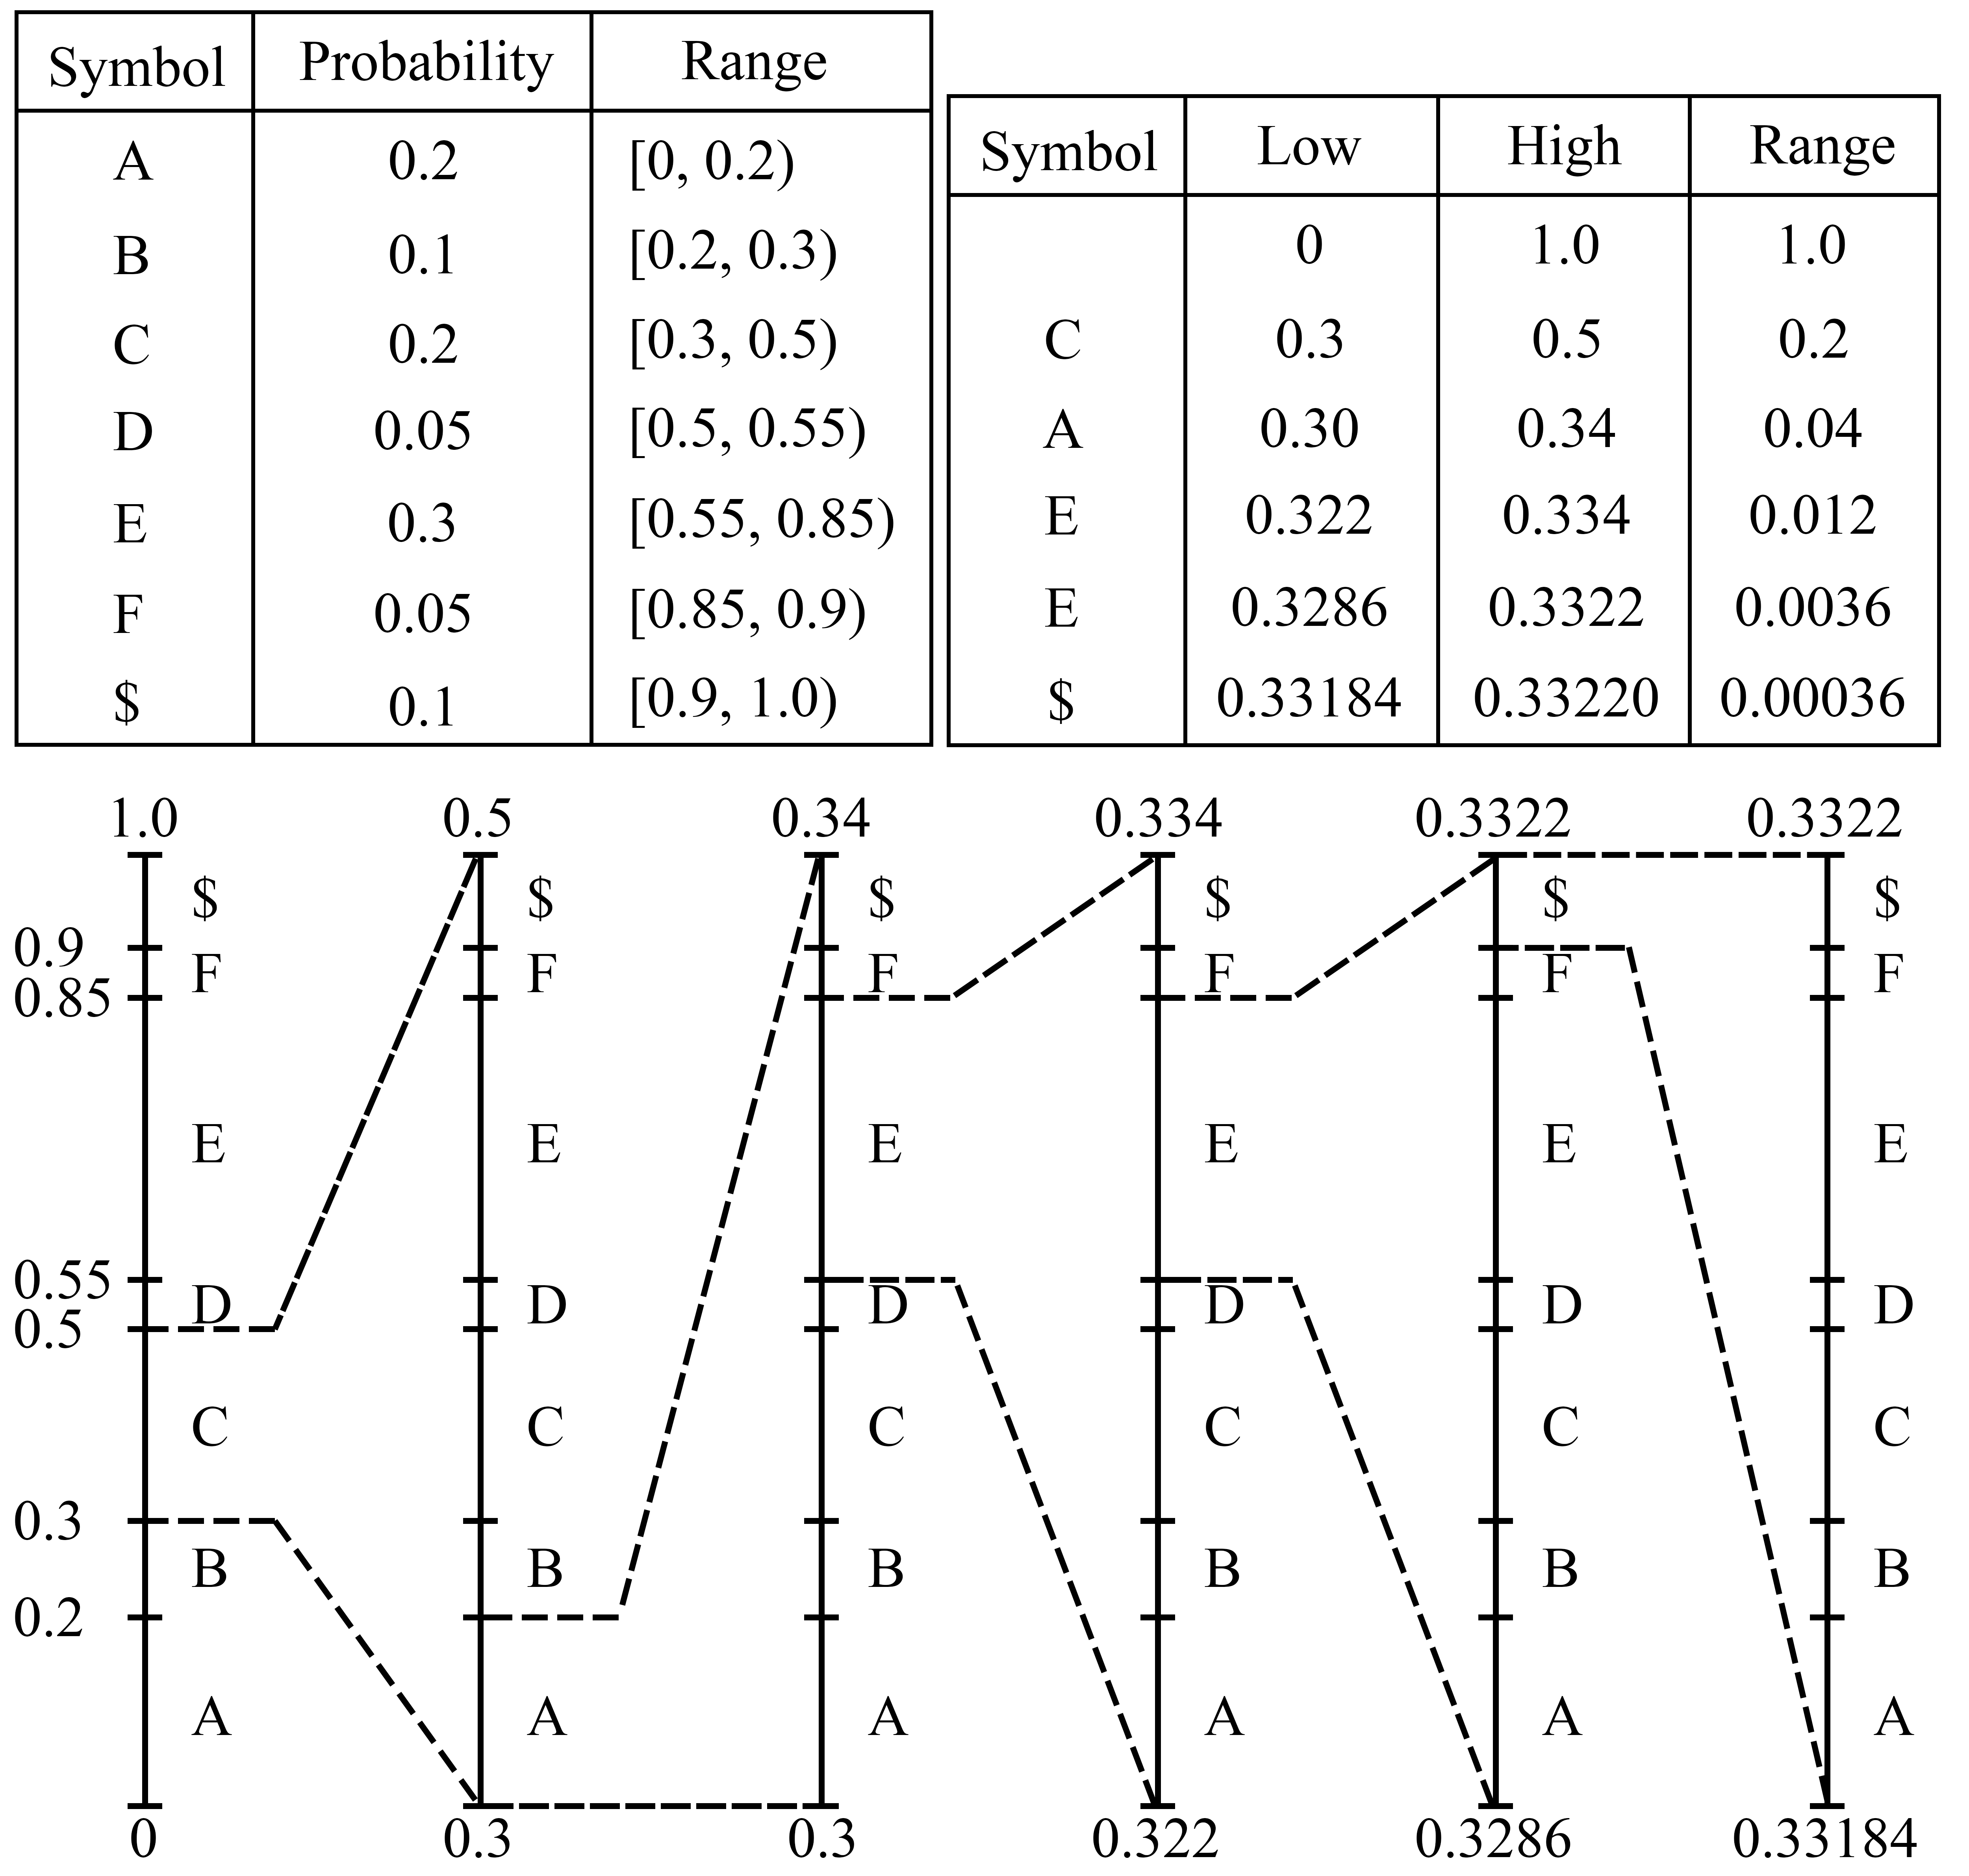
\includegraphics[width=11cm]{images/arithmectic.png}
    \caption{Arithmetic encoding of the character sequence CAEE\$ in the character space ABCDEF\$.}
    \label{img:arith_enco}
\end{figure}


\starsection{Additional Compression Techniques}
\starsubsection{Run-Length Encoding}
Run-Length encoding (RLE) is a lossless encoding scheme that performs well when identical elements frequently appear sequentially. In the sequence AAAABCCCC for example, the characters A and C have adjacent repetitions. Run-Length encoding couples the elements with a number that represents the count of repeated characters. For the example above, the encoding scheme creates the pairs $(\text{A}, 4), (\text{B}, 1), (\text{C}, 4)$ and RLE concatenates the pairs, resulting in an encoding of 4A1B4C.

With its simplicity, RLE provides fast execution, but in most cases RLE results in a lower compression ratio as compared to other algorithms \cite{Sharma2010CompressionUH}. One drawback, as evident by the example above, is that the absence of repetition has to be encoded as well. For text with few repetitions, using RLE will likely increase the size since the gain will be negligible in relation to the overhead. 


\starsubsection{LZ77}
LZ77 is a lossless compression algorithm created by Abraham Lempel and Jacob Ziv in 1977. The intuition behind the algorithm is to remove redundancies of repeated sequences by using pointers to an earlier occurrence of the repetition. 

\begin{figure}[htbp]
    \centering
    \includesvg[width=11cm]{images/lz77.svg}
    \caption{Example of LZ77 encoding of the word sequence \textit{abracadabrad}.}
    \label{img:lz77}
\end{figure}


As illustrated by the example in Figure \ref{img:lz77}, the algorithm uses two sliding windows of predetermined size: a lookahead buffer and a search window. The two windows are aligned, such that the start of the lookahead window is successive to the end of the search window. The idea with the windows is to match the longest sequences in the lookahead buffer, starting at its beginning, with a pointer to the same sequence in the search window. When a match has been found, the two windows shift \(1 + len(match)\) characters along the sequence. A match results in a 3-tuple \textit{(match offset, match length, next nonmatching character)}, which is the output of the algorithm. Decompression is done by performing the process of creating the compressed sequence in reverse \cite{10.1145/356924.356930}. LZ77 is used in current compression algorithms, such as in DEFLATE where it is combined with Huffman encoding. 

\starsubsection{Burrows-Wheeler Transform}
Burrows-Wheeler transform is a method to reorder a string, so the same characters appear sequentially more often. The transformation is invertible, making it possible to go back and forth between the original input string and the transformed version. The invertible property makes it appropriate as a pre-processing step for compression algorithms. For example, Run-Length encoding may perform better when BWT is applied beforehand. To create the Burrows-Wheeler transform, all permutations of the input string, with an inserted marker for the beginning and ending of the string, are generated. The permutations are sorted based on lexical ordering and a sequence containing the last character for each permutation is extracted. As shown in Figure \ref{img:burrow}, the sequence \textit{$\wedge$BANANA $\mid$}, with $\wedge$ and $\mid$ notating the start and end of the sequence, is Burrows-Wheeler transformed into \textit{BNN$\wedge$AA$\mid$A} \cite{Burrows1994ABL}.

\begin{figure}[htbp]
\centering
\resizebox{13cm}{!}{
\begin{tabular}{|lllll|}
\hline
\multicolumn{5}{|c|}{\textbf{Transformation}} \\ \hline
\multicolumn{1}{|c|}{\textbf{Input}} & \multicolumn{1}{c|}{\textbf{All Rotations}} & \multicolumn{1}{c|}{\textbf{Sorting  Rows}} & \multicolumn{1}{c|}{\textbf{Taking Last Column}} & \multicolumn{1}{c|}{\textbf{Output Last Column}} \\ \hline
\multicolumn{1}{|c|}{} & \multicolumn{1}{l|}{\textasciicircum{}BANANA\textcolor{red}{|}} & \multicolumn{1}{l|}{ANANA\textcolor{red}{|}\textasciicircum{}B} & \multicolumn{1}{l|}{ANANA\textcolor{red}{|}\textasciicircum{}\textbf{B}} & \\
\multicolumn{1}{|l|}{} & \multicolumn{1}{l|}{\textcolor{red}{|}\textasciicircum{}BANANA} & \multicolumn{1}{l|}{ANA\textcolor{red}{|}\textasciicircum{}BAN} & \multicolumn{1}{l|}{ANA\textcolor{red}{|}\textasciicircum{}BA\textbf{N}} & \\
\multicolumn{1}{|l|}{} & \multicolumn{1}{l|}{A\textcolor{red}{|}\textasciicircum{}BANAN} & \multicolumn{1}{l|}{A\textcolor{red}{|}\textasciicircum{}BANAN} & \multicolumn{1}{l|}{A\textcolor{red}{|}\textasciicircum{}BANA\textbf{N}} & \\
\multicolumn{1}{|l|}{\textasciicircum{}BANANA\textcolor{red}{|}} & \multicolumn{1}{l|}{NA\textcolor{red}{|}\textasciicircum{}BANA} & \multicolumn{1}{l|}{BANANA\textcolor{red}{|} \textasciicircum{}} & \multicolumn{1}{l|}{BANANA\textcolor{red}{|} \textbf{\textasciicircum{}}} & BNN\textasciicircum{}AA\textcolor{red}{|}A \\
\multicolumn{1}{|l|}{} & \multicolumn{1}{l|}{ANA\textcolor{red}{|}\textasciicircum{}BAN} & \multicolumn{1}{l|}{NANA\textcolor{red}{|}\textasciicircum{}BA} & \multicolumn{1}{l|}{NANA\textcolor{red}{|}\textasciicircum{}B\textbf{A}} & \\
\multicolumn{1}{|l|}{} & \multicolumn{1}{l|}{NANA\textcolor{red}{|}\textasciicircum{}BA} & \multicolumn{1}{l|}{NA\textcolor{red}{|}\textasciicircum{}BANA} & \multicolumn{1}{l|}{NA\textcolor{red}{|}\textasciicircum{}BAN\textbf{A}} & \\
\multicolumn{1}{|l|}{} & \multicolumn{1}{l|}{ANANA\textcolor{red}{|}\textasciicircum{}B} & \multicolumn{1}{l|}{\textasciicircum{}BANANA\textbf{\textcolor{red}{|}}} & \multicolumn{1}{l|}{\textasciicircum{}BANANA\textbf{\textcolor{red}{|}}} & \\
\multicolumn{1}{|l|}{} & \multicolumn{1}{l|}{BANANA\textcolor{red}{|} \textasciicircum{}} & \multicolumn{1}{l|}{\textcolor{red}{|}\textasciicircum{}BANANA} & \multicolumn{1}{l|}{\textcolor{red}{|}\textasciicircum{}BANAN\textbf{A}} & \\ \hline
\end{tabular}}
\caption{Example of Burrows-Wheeler transformation of the sentence \textit{BANANA}.}
    \label{img:burrow}
\end{figure}



\section{Evaluation Metrics}
%https://d1wqtxts1xzle7.cloudfront.net/61774586/Comp_com20200113-81589-6qysrz-libre.pdf?1578974392=&response-content-disposition=inline%3B+filename%3DCOMPARISON_OF_LOSSLESS_DATA_COMPRESSION.pdf&Expires=1676575765&Signature=gBodn-UaNo~-5ZUeGpUiLK66qHtwp1Hw7fLBIJ7LSKGo~40COks2cGmLZdzuRBFDZ1O53ChN8UrCBAwjaz9UqpKodkcPMVgvuYlYsn1mZ6UuF4g4Axpw1fyO5b9YsZGmM-K49J05s88F-WaUtzR0v35MyLW9xl-EQex~Zv1Go9Pcb2v31FYNFfxTPXToR3zZlSACIGXDRm6rVtv3~m9XZTcJPrTCAwbflZPUDWimP5d-oyCiIVFhU5su~-MfKOjk3y0r9huIz-jH~OQu3L~QMBgSH6~3w-aXB8vyXYtjqLil0QuiTaIN64KV7FkPljpMl7k4CXt02uYdu-v0dLSADA__&Key-Pair-Id=APKAJLOHF5GGSLRBV4ZA

The most frequently used evaluation metrics for compression are the \textit{compression ratio} and the \textit{compression factor}, presented in Equation \ref{eq:ratioformula}. The compression ratio describes the output size of a compression algorithm relative to the input data size. For instance, a compression ratio of 0.5 means that the compressed data is 50\% the size of the input. The compression factor is simply the inverse of the compression ratio \cite{metric}. In the industry, it is also common to denote the performance by \(X\):\(1\), where \(X\) is the compression factor \cite{ratioIBM}.

\begin{equation}
    \textrm{\textbf{Compression Ratio}}=\frac{\textrm{1}}
    {\textrm{\textbf{Compression Factor}}}=\frac{\textrm{Size of output stream}}
    {\textrm{Size of input stream}}
    \label{eq:ratioformula}
\end{equation}


Execution time is a metric that is used when evaluating the performance of compression schemes and operations. A problem with simply using the absolute execution time is that it can be influenced by factors that are unrelated to the implementations, such as hardware performance \cite{metric}. To ensure a fair comparison, the relative execution time between different runs under the same circumstances can be compared instead. For this to be reliable, a mean of multiple runs should be considered to filter out noise in the measurements.
Calculating the relative execution time can be done as in Equation \ref{eq:speedformula}.



\begin{equation}
    \textrm{\textbf{Relative Execution Time}}=\frac{\textrm{Time for implementation}}{\textrm{Time for baseline}}
    \label{eq:speedformula}
\end{equation}




\section{Spatial Indexing}
%Indexing generellt: https://medium.com/nerd-for-tech/indexing-data-structures-aa7363693c40
One common challenge when dealing with large amounts of data is efficiently retrieving a subset of the data at an arbitrary location in storage, referred to as \emph{random access} queries. Indexing reduces access time by providing a pointer to the relevant data section based on the input data in the query. Spatial indexing is a subfield that focuses on retrieving data based on a geographic location.
\starsubsection{Quadtrees}
\begin{figure}[h]
    \centering
    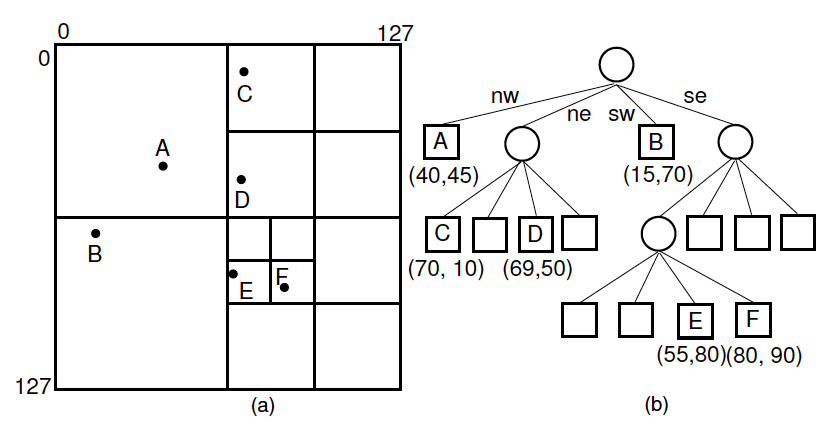
\includegraphics[width=12cm]{images/Point_quadtree.png}
    \caption{An illustration of a quadtree structure in a plane of points. The notation of nw, ne, sw, and se in the tree structure corresponds to the top left, top right, bottom left, and bottom right quadrants, respectively \cite[Figure~13.6]{huffman_tree_img}.} %Same book as huffman img
    \label{img:quad}
\end{figure}
% Riktigt bra sammanfattning av olika indexeringsmetoder
%http://www.cs.siue.edu/~marmcke/docs/cs490/spatialIndexing.html
A quadtree is a hierarchical tree structure where each node has zero or four children. The hierarchical structure enables indexing and makes querying for specific regions of the two-dimensional space convenient.

In a quadtree, each node describes a section of a two-dimensional plane, where the root node describes the section in its entirety. The intuition behind the quadtree is that for a non-leaf node, its four children divide the parent node's two-dimensional section into four quadrants \cite{10.1145/356924.356930}, see Figure \ref{img:quad}.

If a quadrant does not split the data, there is no reason to further divide the section of a node, and it can be assigned as a leaf node. Additionally, the algorithm can stop creating quadrants when a node contains a specified maximum number of data points \cite{10.1145/356924.356930}.


\chapter{Methodology}
In this chapter the iterative work process, data collection, and the technical tools used during development are explained.
\section{Work Process}
% Olika faser:
% Inläsning, hämta grundläggande data, använd färdiga algos, implementera baseline, extend upon baseline
% enklare operationr först, sedan påbörja svårare

The methodology used for the thesis is a mixture of reading prior literature on common compression algorithms, spatial operations, and floating-point representations. Along with data collection and preprocessing, implementing benchmarking and validation environments, and iteratively implementing and evaluating ideas obtained through brainstorming and combining existing literature. When ideas were proposed, the potential gain and estimated implementation complexity were used to rank the development order. Thus, some ideas were never implemented due to time constraints, but the ideas are still documented in the report for future reference.   

A rough overview of the process used during the 20 weeks of the thesis is presented below:
\begin{enumerate}

  \item Look into different sources for open-source map data where the geometrical object format is known. When decided, incorporate the data into an existing geometric framework, such as \emph{Shapely}, and become familiar with the formats. Set up an environment for testing, developing, and evaluating implementations of compression algorithms performing geometric operations on the processed data.
    
  \item Conduct a literature review of compression concepts and encoding of geometries consisting of floating-point coordinates. Investigate what kind of algorithms are suitable for geometrical map data.

  \item Implement one baseline algorithm which can be extended. The baseline should perform the geometric operations by decompressing the whole geometry, and the algorithm should be relevant in the field of maps compression.
  
  \item Change the underlying structure of the baseline to enable unary and binary operations by partial decompression. Performed by iteratively coming up with new ideas, implementing them, and measuring the performance difference between the algorithms in terms of efficiency and storage space.

  \item Examine how the compression ratio can be optimized while preserving the operability, by exploiting the maps domain and applying a combination of known compression strategies. Also, improve execution time by utilizing profiling tools and optimizing the implementation.


\end{enumerate}


\section{Establishing the Baseline}
Due to the significant performance differences between programming languages, such as C and Python, programming language consistency is critical to ensure a fair comparison between implementations. As mentioned in Section \ref{scopeLimit},  the implementation of our compression format is written in Python, and for conducting fair performance assessments, an appropriate baseline was re-implemented in Python. The baseline provides a base for evaluation, and by comparing the relative performance scoring between different implementations, an idea of their general performance can be extrapolated. 

For instance, if implemented in the same programming language, comparing the execution time of a baseline that decompresses an entire geometry with the execution time of an operation-integrated compression format with support for partial decompression, valid data on the performance benefits of partial decompression can be obtained. However, if the operations are done in different languages, the effect of the different languages cannot be controlled.

Nonetheless, there are situations where valuable insights can be gained by comparing operations written in \textit{partially different} languages. If an operation-integrated compression format outperforms the complete operation, which includes decompression and a library function in the baseline, and both use the same programming language for the decompression, despite the possibility that the baseline might utilize a more efficient library function, the operation-integrated compression format demonstrates its superiority by outperforming the baseline in overall time.

\section{Supported Operations}
There exist many operations which can be used to manipulate or extract information from geometries. To narrow the scope of the thesis, the supervisors proposed some operations that are often performed on GIS data. Three distinct operations were chosen as the primary goals of optimization: \emph{bounding box}, \emph{add vertex}, and \emph{intersection} (both \emph{predicate} and \emph{boolean}). The operations are characterized by being \emph{constant}, \emph{modifying}, and \emph{binary} operations, respectively.
\\\\
During meetings with the supervisors, the following unary operations were proposed as interesting and while only a few are in focus for the thesis, the others may be integrated and optimized in future work:
\begin{description}
    \item[Vertex Count] Number of total vertices.
    \item[Area] For polygons, the total area minus the area of the holes.
    \item[Length] Total length for linestrings, circumference for polygons.
    \item[Modify Vertices] Add, remove, edit individual vertices.
    \item[Bounding Box] Returns the corners of the minimum axis-aligned rectangle such that all vertices in the shape are contained.
    \item[Buffering/Scaling] Change the size of the geometry while preserving the center of mass and proportions. 
    \item[Convex Hull] The smallest convex set containing the shape.
    \item[Center of Mass] Average position of all vertices.
    \item[End-Points] For linestrings only.
\end{description}

For \emph{binary operations}, the spatial predicates which can be derived from the DE-9IM model, such as \emph{intersects} and \emph{contains}, along with the boolean operations of \emph{intersection}, and \emph{union}, returning a shape, were proposed as operations to be optimized.

\section{Datasets \& Preprocessing}
\label{sec:datasets}
Spatial datasets are used to evaluate the performance of the implementations. This section provides an overview of the data sources used and the preprocessing steps performed on them.
\begin{figure}[H]%
    \centering
    \subfloat[\centering Buildings in red and roads in blue.]{{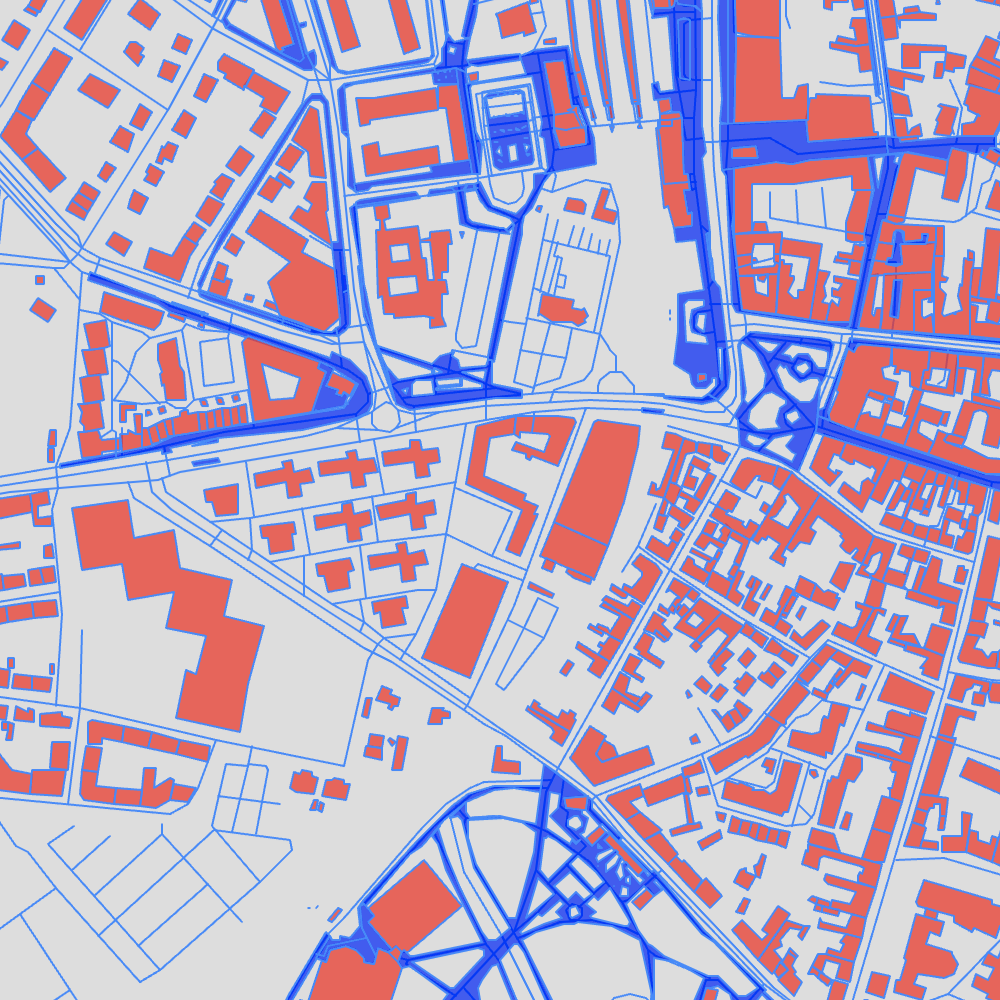
\includegraphics[width=6.9cm]{images/building_road.png} }}%
    \qquad
    \subfloat[\centering Administrative borders.]{{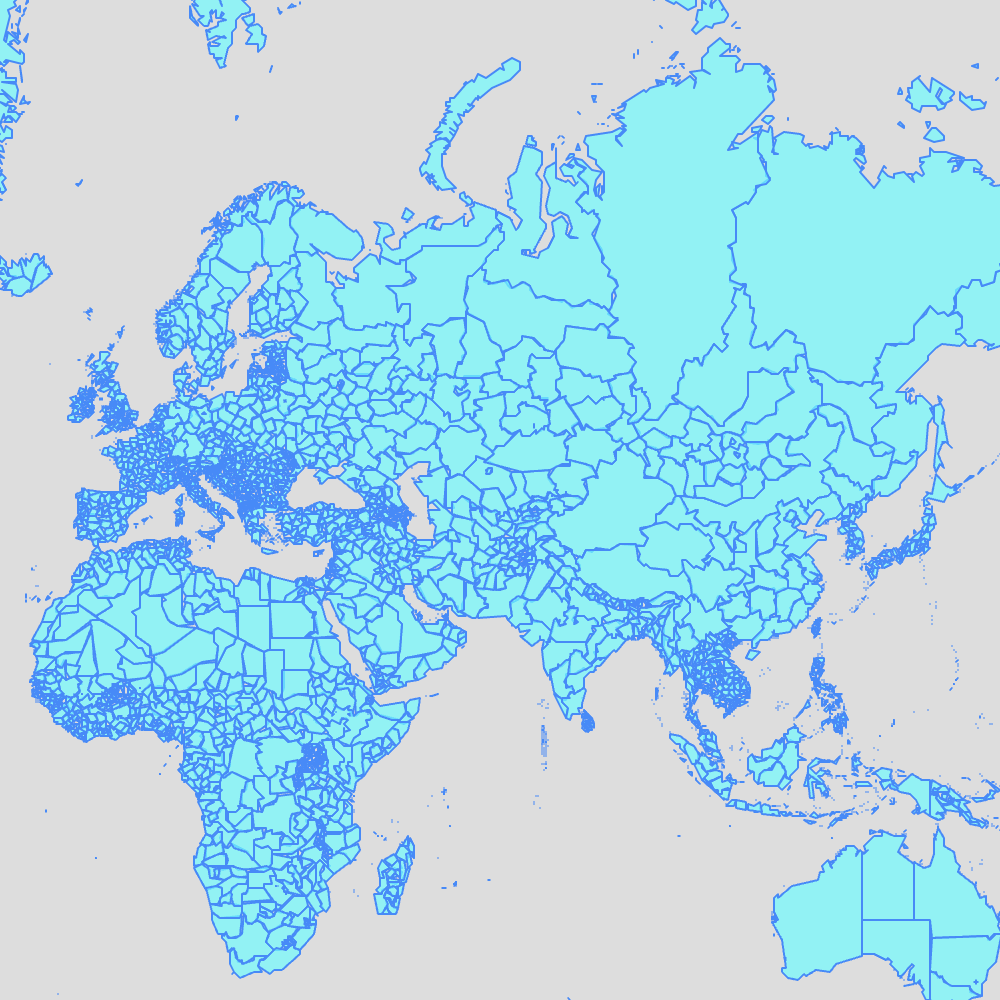
\includegraphics[width=6.9cm]{images/countries.png} }{\label{fig:adminexamp}}}%
    \caption{Excerpts from the datasets used for benchmarking.}%
    \label{fig:datapreview}%
\end{figure}

\subsection{OpenStreetMap}
OpenStreetMap (OSM) is an open-source database for spatial data covering the whole world. It is licensed under Open Database License (ODBL), which allows the user to use the data with little restrictions to copyright and ownership rights. The flexibility of ODBL implies that it is permitted for users to create, share and modify the data \cite{osmlicense}. 

% There exist sources with more extensive coverage than OpenStreetMap, but for the sake of this investigation, OSM's content is enough, together with the significant perk of its license flexibility.

% \todo{Till Leo: "There exist sources with more extensive coverage than OpenStreetMap": stämmer det? I så fall var hittade du det?}

The format of OSM can be divided into four categories: nodes, ways, relations, and tags. Nodes describe specific coordinate points of a map; ways is a polyline or a polygon of an ordered sequence of nodes; relations combine nodes, ways, and recursive relations to form larger map-related structures; and lastly, tags are metadata to any type containing extra information about objects \cite{osm_datastructure}.

Due to OSM containing shapes covering a large portion of the world, it is impractical to work with the entire dataset. Instead, extractions from the dataset were downloaded through Geofabrik, an OpenStreetMap data extract provider. Different extracts were considered to investigate how the performance of the implementation is affected by the characteristics of the datasets.

Four datasets: \emph{Sweden Buildings}, \emph{Sweden Roads}, \emph{Sweden All}, and \emph{China Water} were selected to be used in the evaluation. Buildings and roads were selected since they are both common geometries, but the shapes are usually different. \emph{China Water} was selected because geometries representing water (lakes, rivers, streams) usually have a high vertex count, and using data from different countries can reduce the bias induced by geographical differences. Characteristics and images of the datasets are available in Table \ref{tab:dataset_stats}, Figure \ref{fig:datapreview}, and Figure \ref{img:data_distrb_all}.

\subsection{Database of Global Administrative Areas}
The Database of Global Administrative Areas (GADM) is a maps data provider with the goal of mapping all administrative areas of all countries, at all levels of sub-division \cite{gadm}. GADM is freely available for academic use and other non-commercial use. Due to the number of vertices in the shapes, the borders of all administrative areas, as visible in Figure \ref{fig:adminexamp}, are used in the evaluation.


\begin{table}[H]
\centering
\caption{Characteristics of datasets.} 
\label{tab:dataset_stats}
\resizebox{\textwidth}{!}{%

\begin{tabular}{@{\extracolsep{4pt}}lcccccc}
\toprule   
 {} & {} & \multicolumn{3}{c}{Type Distribution (\%)}  & \multicolumn{2}{c}{$\mathrel\#$ Vertices}\\
 \cmidrule{3-5} 
 \cmidrule{6-7} 
Dataset & $\mathrel\#$ Geometries & LineString & Polygon & MultiPolygon & Total & Average \\ 
\midrule
Sweden Buildings & 2.8M & - & 99.9 & 0.1 & 17.8M & 6.3 \\ 
Sweden Roads & 1.9M & 100 & - & - & 24.1M & 12.7  \\
Sweden All & 6.4M & 31.9 & 68 & 0.1 & 104.5M & 16.4  \\ 
China Water & 367K & - & 99.7 & 0.3 & 21.8M & 59  \\ 
Admin Borders & 4596 & - & 85.8 & 14.2 & 1.3M & 282  \\ 
\bottomrule
\end{tabular}}
\end{table}

\begin{figure}[htbp]
    \centering
    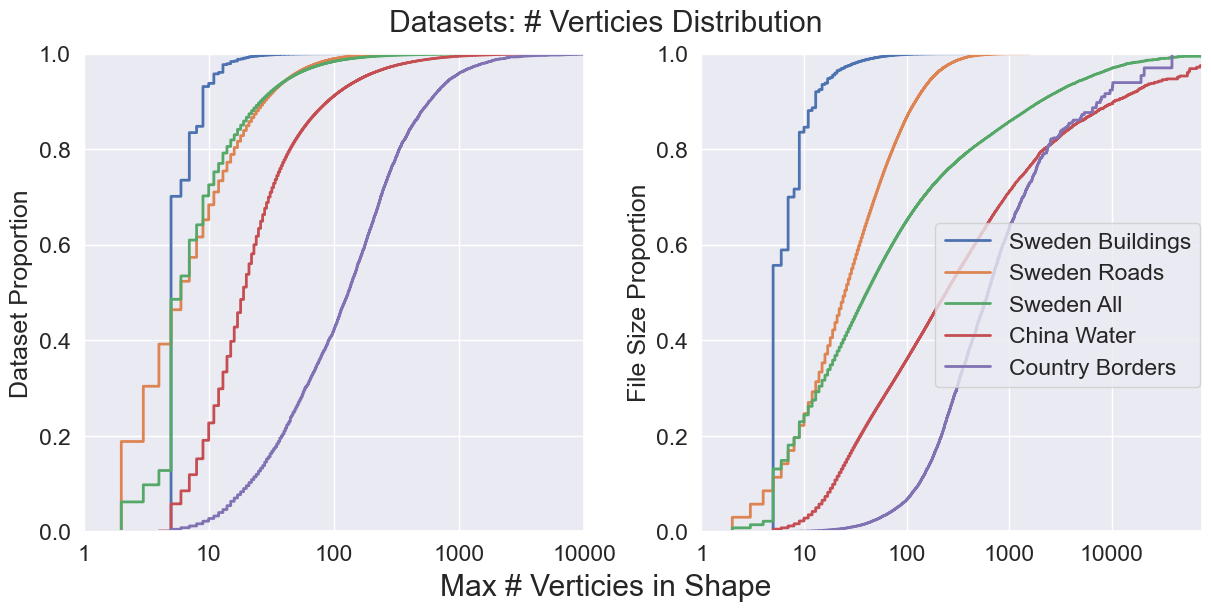
\includegraphics[width=14.5cm]{images/data_distrb_all.png}
    \caption{Cumulative distribution of the vertex count for the geometries based on the dataset. The right plot is weighted by the number of vertices, indicating how the overall size is distributed. For example, the size of one shape containing 30 vertices is equal to 6 shapes containing 5 vertices.}
        \label{img:data_distrb_all}
\end{figure}

%För varje:
%Antal punkter avg
%Tot points, avg points per shape
%https://texblog.org/2017/02/06/proper-tables-with-latex/
%https://tex.stackexchange.com/questions/380233/how-to-manually-make-tables-using-booktabs





\subsection{Intersection Data}
\label{sec:intersectiondataintro}
In order to benchmark the operations of intersection, datasets consisting of pairs of shapes resulting in the different cases of intersection are needed.

\subsubsection{OSM \& GADM}
The common case for intersection, if picking two geometries at random, is that no intersection occurs. To collect the queries of interest, the bounding boxes of all shapes were pairwise tested for intersection, and the queries containing an intersection were kept. In addition to the case of \emph{no intersection}, the possible distinct cases when the bounding boxes intersect are \emph{no intersection}, \emph{intersection with crossing segments}, and \emph{intersection by contains}.

The testing was performed for all shapes in \emph{Admin Borders}, for all shapes of type building or highway (used for identifying any kind of road, street or path) in the city of Lund (subset of \emph{Sweden All}), and random subsets of 100 000 queries from \emph{Sweden All} and \emph{China Water}.

\subsubsection{Manually Created Special Cases}
Since the shapes can consist of polylines, polygons, polygons with holes, and multipolygons, there exist numerous possible relations between the types of the intersecting shapes. Furthermore, a number of edge cases, such as shapes consisting of parallel lines, have to be accounted for when implementing intersection. In order to test for those, along with the possible worst- and best-case scenarios, the GIS editing tool \emph{QGIS} was used to manually create a dataset of such shapes.

\section{Validation \& Benchmarking Environment}
A test bench was created in order to evaluate and verify the different implementations of compression algorithms and their operations. Due to Python's large number of existing modules and community support, the test bench was written as a Python \emph{Jupyter Notebook}. By being able to split code into cells and have the output from each cell presented directly under the code, Jupyter Notebooks can be used to present both code and plots of results in a structured manner.
\\\\
To allow for fast integration of new or altered algorithm implementations, the test bench was written in a generalized manner, being as decoupled from the algorithm implementation as possible. This was achieved by having an abstract base class that consists of the methods for compression, decompression, and the corresponding operations. Each algorithm derives from the base class and provides implementations of the abstract methods. With this setup, a new algorithm can be added by simply changing one line in the test bench. Furthermore, the dataset used in the benchmarking can also be specified by changing one configuration variable.

%https://docs.google.com/viewer?a=v&pid=sites&srcid=ZGVmYXVsdGRvbWFpbnx0ZXN0MTIzNHNpbTQ2NXxneDpiYTJmYWIwYTAyOGJiZmQ
\subsection{Validation of Operations}
Test-driven development is a common strategy used to maintain system correctness over time. By shortening the feedback loop in the form of automated testing, bugs in implementations can be caught in a matter of seconds \cite{tdd}.

For lossless compression algorithms, one obvious test case is verifying that the decompressed data is equal to the original data. When dealing with geometric data, it is also the case that all operations should exhibit the same behavior in the geometry space, regardless of the algorithm used. When modifying geometries, one way to validate operation correctness is to perform the operation on the compressed data using the untested algorithm and then decompress the data altogether and compare the output with a trusted implementation.
\\\\
To ensure the correctness of the implemented algorithms in the thesis, a validation section is included in the test bench. During benchmarking, each query and its corresponding result are logged. After executing all queries, the queries are re-run using a verified implementation, and the outputs are compared to ensure consistency.

\subsection{Shapely}
Comparison fairness is essential when benchmarking different compression algorithms. Therefore, all algorithms assume the same input and output format. The Python GEOS library \emph{Shapely} is used as the algorithms' start and end point format. Shapely comes with a spatial data model supporting common functionalities. The premise of Shapely is its convenience for working with and operating on spatial objects without the need for relational databases \cite{shapely}.

All the geometries described in the theoretical background, such as Point, LineString, Polygon, and MultiPolygon, are available as geometric Python objects supporting various spatial operations. Additionally, Shapely is compatible with common formats, such as WKT, WKB, and GeoJSON, making working with online datasets convenient \cite{shapely}.

\begin{figure}[htbp]
    \centering
    \includesvg[width=15cm]{images/Benchmarking diagram.svg}
    \caption{Visualization overview of the benchmarking pipeline. Orange boxes indicate values passed to benchmarking or validation and \textit{ALG} is the current  algorithm to test.}
    \label{img:bench}
\end{figure}

\subsection{Benchmarking}
For benchmarking the algorithms, it is assumed that all the input data for the algorithms are stored in RAM, and benchmarking does not include the overhead of reading and writing data to storage. This enhances a fair comparison by removing the impact on performance caused by the storage solution. The compression, decompression, and operations assume three different starting and ending premises:
\begin{itemize}
    \item \textbf{Compress: }Shapely object $\xrightarrow{output}$ Binary String  
    \item \textbf{Decompress: }Binary String $\xrightarrow{output}$ Shapely Object    
    \item \textbf{Operations: }Binary String $\xrightarrow{output}$ Value/Binary String
\end{itemize}

Since the third-party library Shapely is used for the algorithms, consistency of its use between the different algorithms must be considered. For instance, there are various ways of instantiating Shapely objects. Suppose that different Shapely object creation strategies are used for different algorithms. In that case, the benchmarking comparison might be unfair since the relative efficiency differences between the methods in the third-party library are unknown.

The common benchmarks for compression, decompression, and operations are running time. For compression and decompression, the size differences in bytes for the different algorithms are also investigated.  In Figure \ref{img:bench}, the pipeline for benchmarking the algorithms can be seen.


% \todo{större text, ta bort att tid mäts i operations. Döpa om "operations" till Validation?}


\subsection{Performance Profiling}Due to Python being an interpreted language and lacking an optimizing compiler, profiling is essential for finding implementation bottlenecks. The Python profiling tool \emph{Kernprof}, together with its complement \emph{line\_profiler}, can be used to extract line-by-line statistics for different functions. For each line, the statistics contain the number of hits, the accumulated execution time, and its corresponding time percentage relative to the encapsulating function \cite{kernprof}.

In addition to locating slow code, profiling provides algorithmic insight. When developing algorithms, understanding which parts are logically flawed or time-consuming is valuable for creating efficient and robust algorithms. 
%compress: shapely -> bin, decomp: bin -> shapely, %operations: bin -> value/bin
%Avoid file reading/writing part of time. %To/from_ragged_array in Shapely for consistency



\chapter{Algorithm Implementations}
\label{sec:chapterimplementation}
This chapter consists of implementing support for the standard geometry file formats, re-implementing the baseline, and descriptions of extensions that provide operability support for the baseline.

\section{WKT, WKB \& Gzip}
% Kort om våra första implementationer. Dessa jämförs ju inte sen då de är en invalid baseline. Men kan ändå vara bra att nämna lite
WKB is used as the reference when verifying the correctness of the implementations, and for size benchmarking, while WKT is convenient to use when debugging. Additionally, due to its smaller size and higher performance, WKB is commonly used in the industry. Therefore, classes utilizing Shapely for parsing and serializing WKT and WKB were written to support the benchmarking environment.
\\\\
Python includes support for working with most common compression formats, including the general-purpose formats \emph{gzip}, \emph{zlib}, and \emph{bzip2}. Classes consisting of serialization to WKB and WKT followed by compression using algorithms provided by the Python library were implemented in order to compare the compression ratios.


\section{Baseline: Floating-Point Delta}
\label{section:baseline}
As described in the related work section, floating-point delta (FPD) encoding is a compression algorithm suited for spatial data. Due to its simplicity while still being related to the spatial domain, the algorithm \cite{spatialparquet} serves as the baseline in this thesis.

Our implementation of FP-delta encoding, similar to \citeauthor{spatialparquet}'s implementation \emph{Spatial Parquet}, consists of one pre-iteration over the geometry in order to determine the optimal bit-length of the deltas, followed by interpreting the floating-point values as signed integers, and zigzag encoding the consecutive differences between the corresponding $(x, y)$ pairs. If either the x- or y-value overflows, a new chunk is created.

\begin{figure}[htbp]
    \centering
    \includesvg[width=15cm]{images/FP-Delta implementation.svg}
    \caption{Visualization overview of the bit structure of the FP-delta baseline format.}
    \label{img:fp_delta_base}
\end{figure}

Due to the differences between the underlying file formats, where Spatial Parquet is based on the Parquet standard, and the thesis on standalone files for each geometry, the encoding of the different geometry types differs between the implementations. The baseline format, as outlined in Figure \ref{img:fp_delta_base}, starts with two integers; the \textit{delta size} and the \textit{geometry type}, followed by a number of chunks that contain chunk metadata, required for parsing the geometry structure, and coordinate pairs. During parsing, the metadata is used to determine the context and length of the corresponding chunks, allowing for the reconstruction of the individual parts of the geometries. As also seen in the figure, the metadata differs between the geometry types and consists of:
\begin{itemize}
    \item \textbf{LineString}: the number of deltas in the current chunk.
    \item \textbf{Polygon}: + the number of chunks for the current ring.
    \item \textbf{MultiPolygon}: + the number of rings for the current polygon.
\end{itemize}

The geometric operations are implemented by decompressing the entire geometries, followed by executing either Shapely's built-in functions when it is sufficient to make a conclusion, or a self-made Python implementation of the operation. The latter is the approach utilized for \emph{Add Vertex}, \textit{Is Intersection} and \textit{Intersection}.


%\todo{byt namn på Chunk size till att det är antalet deltas som lagras, }


\section{Floating-Point Delta Extended}
In this section, we propose and implement enhancements to the geometric operations based on the FP-delta encoding. One motivation for the placement of the baseline's chunk metadata is to allow for further extension of the algorithm, enabling local decompression to improve the effectiveness of the operations. Throughout the report, our implementation is referred to as \emph{Floating-Point Delta Extended}, and abbreviated as \emph{FPDE}. Some of the ideas proposed below were not implemented due to time constraints, but may be of interest when conducting future research; they are marked with an asterisk (*) in the title of the section and can be skipped if the reader is only interested in the implemented concepts.

\subsection{High-Level Structure of the Format}
% Parsing data
% Chunk concept
% How are deltas encoded/decoded (chain)

\begin{figure}[htbp]
    \centering
    \includesvg[width=17.5cm]{images/fpde.svg}
    \caption{Visualization of the implemented structure for our solution. Extending the structure in Figure \ref{img:fp_delta_base}.}
    \label{img:fpde_structure}
\end{figure}

The final structure of the compression format, as seen in Figure \ref{img:fpde_structure}, is similar to the baseline, but both the global and chunk headers have been extended to allow for compressed computation. In summary, the implementation consists of a global header including the \emph{delta size}, \emph{geometry type}, \emph{entropy coding parameter}, \emph{chunk count}, \emph{chunk bounding boxes}, and the \emph{shape bounding box}. The global header is then followed by a sequence of chunks, where the chunk headers as previously contain the parsing data. If entropy encoding is applied, the size of each delta may vary, and to allow for skipping of irrelevant chunks, the total number of bits in each chunk is stored in the chunk header.

\begin{figure}[htbp]
    \centering
    \hspace*{0.5cm} 
    \includesvg[width=15.2cm]{images/flow_chart.svg}
    \caption{High-level flow chart of the compression and decompression operations in FPDE.}
    \label{fig:flow_chart}
\end{figure}


A high-level flow chart is presented in Figure \ref{fig:flow_chart} below, illustrating the sequential steps involved in the compression and decompression operations of the format. As for the baseline, the resulting size of different delta bit-lengths are calculated and the size optimal bit-length is assigned to the shape during compression. Two examples of how the resulting shape size varies with the delta bit-length can be seen in Figure \ref{fig:preiteration}. The chunk bounding boxes, required for the optimized intersection operations, and the global bounding box are calculated during compression. In addition, a maximum chunk size, which forces the creation of a new chunk when a certain number of deltas have been reached, can be specified as a configuration variable. As also visible in the flow chart, the format can configured to use one of three different floating-point encoding techniques, which are explained later in Section \ref{sec:delta_mod}.

\begin{figure}[htbp]%
    \centering
    \subfloat[\centering Shape from \emph{Sweden All}.]{{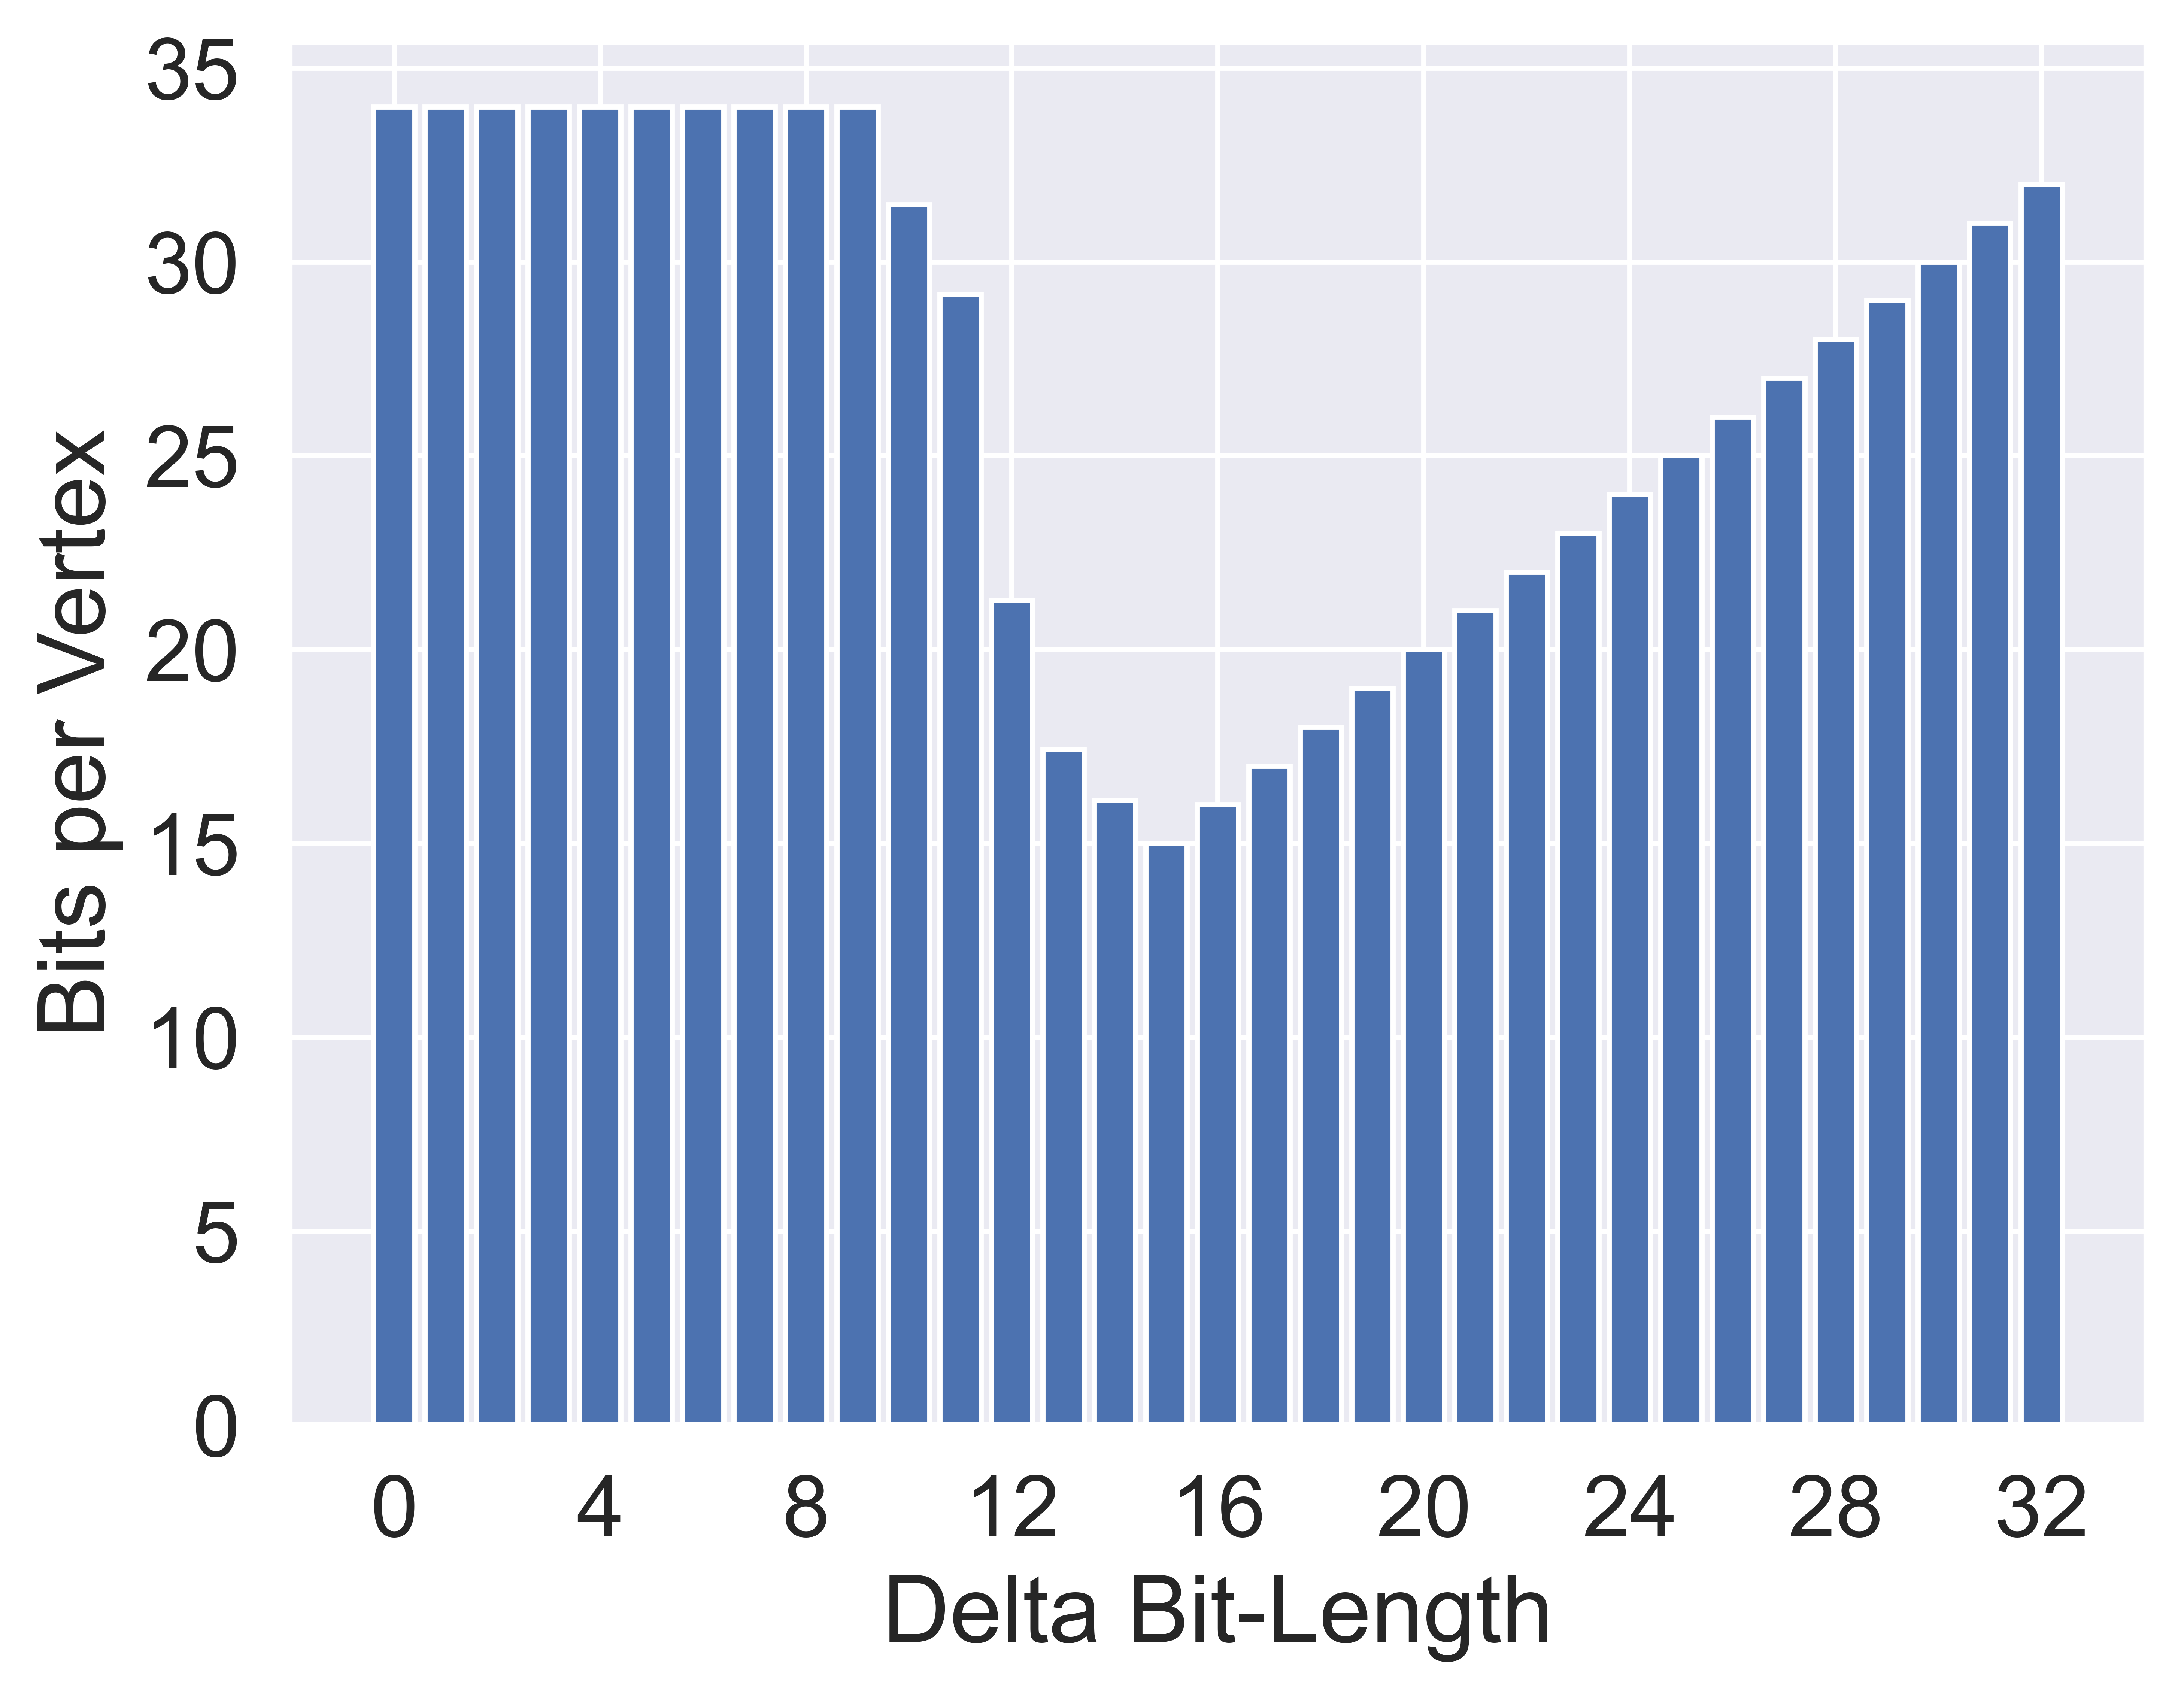
\includegraphics[width=6.9cm]{images/total_size_per_bit_size_sweden.png} }}%
    \qquad
    \subfloat[\centering  Shape from \emph{Admin Borders}.]{{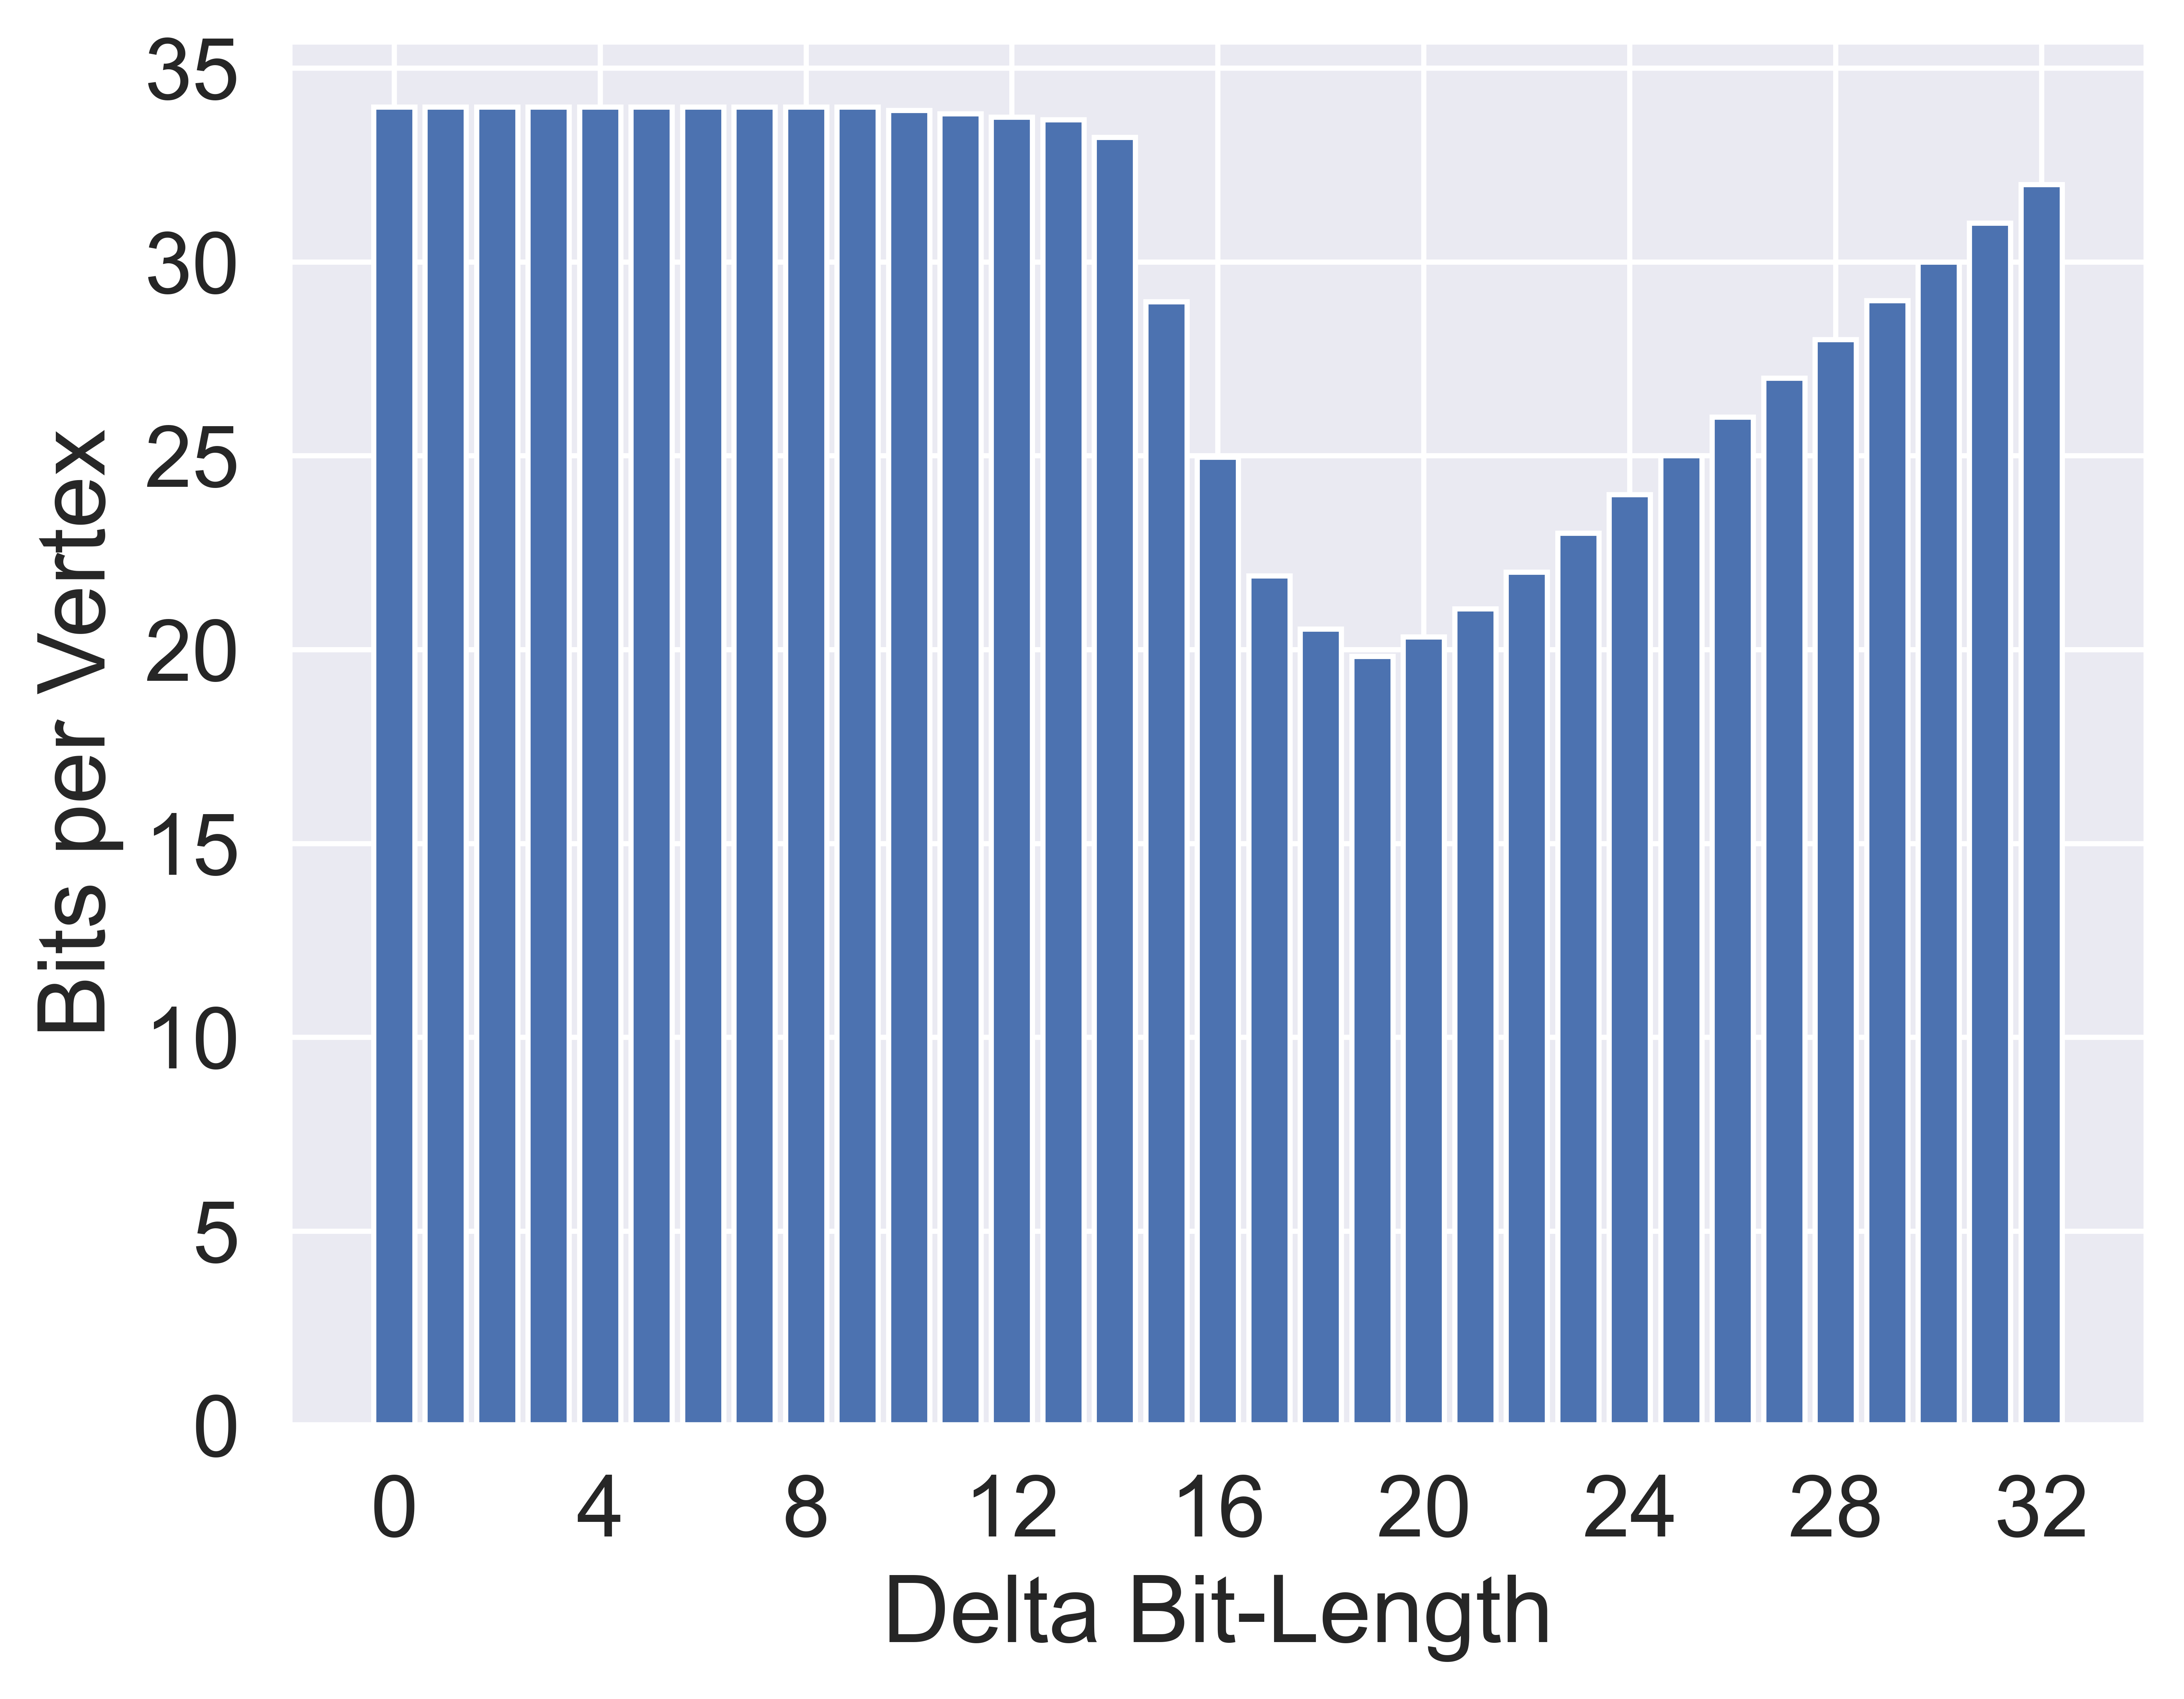
\includegraphics[width=6.9cm]{images/total_size_per_bit_size_world.png} }}%
    \caption{Combined size of all coordinates and chunk headers divided by the vertex count for different delta bit sizes. The figures show the data for two random geometries.}%
    \label{fig:preiteration}%
\end{figure}


% Baseline: Presentera statistik om data, diagram ex. Antal vertices
% Mätningar på vad som tar tid och plats
\section{Bounding Box}\label{boundingbox}
\begin{figure}[htbp]
    \centering
    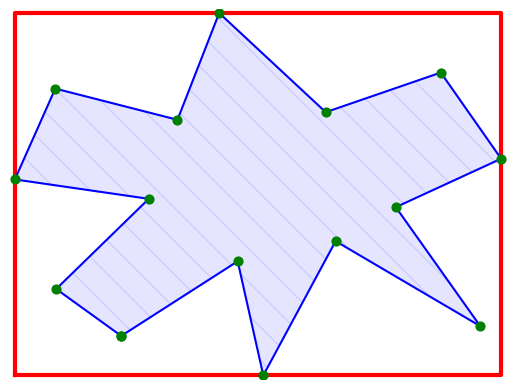
\includegraphics[width=5cm]{images/bbox_example.png}
    \caption{The red rectangle is the bounding box of the shape.}
    \label{fig:bboxexample}
\end{figure}

The minimal axis-aligned rectangle such that all points within the shape are contained is commonly referred to as the \emph{bounding box}. The bounding box can be used as a first step to filter out candidates for further operations. Since all points belonging to the shape are per definition within the bounding box, it can be used as a spatial upper bound for approximating the shape, implying that the shape is at maximum as large as the bounding box. For instance, the intersection operation can be optimized if there is no intersection between the bounding boxes, since this implies that no intersection can possibly occur between the shapes. An example of a bounding box can be seen in Figure \ref{fig:bboxexample}. 

Due to the bounding boxes commonly being used as a first filtration step, it is of great importance that the latency for fetching the bounding box is the lowest possible. Below, a number of implementations for storing and retrieving the bounding boxes are proposed. In FPDE, only the first approach is implemented and evaluated (Section \ref{sec:bboxfull}).

\subsection{Store Full Coordinates}\label{sec:bboxfull}
The first approach is to pre-compute the bounding box and store the bounds, essentially storing two diagonal corner points of the box, resulting in a total of four coordinates. As seen in Equation \ref{eq:bbmeta}, the coordinates of the bounding box are calculated by finding the minimum and maximum values of the X- and Y-vectors of the shape's vertices.
\begin{equation}
    bounds(s)=[\min(xs(s)),\ \max(xs(s)),\ \min(ys(s)),\ \max(ys(s))] = [x_l,\ x_r,\ y_b,\ y_t]
    \label{eq:bbmeta}
\end{equation}

The added overhead from the four coordinates results in a total space of $4 \cdot b_f$ where $b_f$ is the number of bits required to store one coordinate. The value of $b_f$ depends on the format used for serialization of the floating-point coordinates. If using double-precision, the resulting size is $4 \cdot 64 = 256$ bits.

Since the coordinates are stored in full, obtaining the actual bounding box from the memory address can be done in $\mathcal{O}(1)$.

\starsubsection{Store Indices for Spanning Points}
As seen in Equation \ref{eq:bbmeta}, the bounds are defined by a maximum of four unique vertices spanning the bounding box. Instead of storing the full coordinates separately, the overhead can be reduced by storing the indices of the vertices, resulting in Equation \ref{eq:bbind}.
\begin{equation}
    \label{eq:bbind}
    \begin{gathered}
    bounds(s)=[\arg \min(xs(s)),\ \arg \max(xs(s)),\ \arg \min(ys(s)),\ \arg \max(ys(s))] \\
    = [i_{xl},\ i_{xr},\ i_{yb},\ i_{yt}]
    \end{gathered}
\end{equation}
The bounding box can be calculated by retrieving the points based on the indices and taking the $x$- or $y$-coordinate based on the position within the bounds data.

This approach usually requires less space compared to storing the full coordinates, but has a slower query time. To store the indices $4 \cdot \lceil \log_2(V) \rceil$ bits are required. Meaning that with a larger number of vertices, more bits are required. Calculating the bounding box can be done in 
$4 \cdot T(random\_access)$ operations.

\starsubsection{Utilize Sorted List}
If the compressed shape's data structure already includes two lists with indexes or coordinates sorted by x- and y-values, the bounding box can be easily retrieved. Obviously, the sorted lists should not be included for the bounding box alone, but some other operations, such as the first method presented for intersection in Section \ref{sec:intersection}, require sorting.

In this case, no \emph{additional} overhead is added, and if the sorted lists contain indices, retrieving the actual bounding box can be done in $4 \cdot T(random\_access)$ operations. If the sorted lists contain delta encoded coordinates, the time complexity becomes $2 \cdot \mathcal{O}(1) + 2 \cdot T(random\_access)$; where the accesses to $x_l$ and $y_b$ are constant, since they are stored in full at the very beginning of the sorted lists. For $x_r$ and $y_t$, which are stored at the very end of the lists, the accesses are the worst-case for random access. In this case, the access has to loop over all chunk headers and decompress the entire final chunk. Resulting in $T(random\_access) = c_s + m_c$, where $c_s$ is the number of chunks, and $m_c$ is the number of deltas within the last chunk. An improved approach for random access is discussed in Section \ref{sec:optrandom}. 

\starsubsection{Quadtree Approximation}
\label{sec:quadtreeapproximation}
If the exact bounding box is not required, storing it directly can be avoided by using a quadtree. In this case, each bounding box in a set of bounding boxes is part of one of the nodes within the tree. Namely, the node with the largest depth such that the bounding box is fully contained within the quadrant. In libraries for storing and retrieving geometries, spatial indexing commonly uses a tree-like structure based on the bounding boxes of the shapes \cite{spatialindexing}. In such cases, it may be possible to retrieve which quadrant the shape is assigned to from the library. The bounds of the quadrant can then be used as the bounding box approximation.

As this thesis focuses on singular geometries, no spatial indexing is available for the shapes. However, Section \ref{sec:quadtreechunk} proposes a method to reduce the query time and data overhead of operations by employing a quadtree. In this approach, the quadtree approximation of the bounding boxes of the individual chunks within a shape is used, as opposed to storing the coordinates of all the chunks' bounding boxes in full.

% Används i andra operationer, bör vara snabb
% 1.Lagra koordinater för sig
% 2.Lagra index till koordinater som spänner bounding boxen
% 4.Quadtree approximation
% 3.Sorted lista av koordinater: behöver spara winding order

\section{Add Vertex}
In this thesis, \emph{Add Vertex} refers to the operation of inserting a point at a specific index in the shape, with a binary string as output. This represents the operation in \ref{eq:add_vertex_op}:
\begin{equation}
    Add\_Vertex(\emph{bin}_{\emph{in}},\ \emph{idx},\ \emph{point}) \xrightarrow{output} \emph{bin}_{\emph{res}} 
    \label{eq:add_vertex_op}
\end{equation}

\subsection{Indexing Scheme}
For shapes representing at least one polygon, simply using the vertex's index to determine the location of the new vertex can result in ambiguities. Two problems cause the ambiguities to arise:
\begin{enumerate}
    \item Irregular standards regarding if the first point should be equal to the last point in each ring, such that the coordinates form a closed path. Otherwise, the last line segment in each ring is formed implicitly.
    \item Between two rings, it is not clear whether the index is a part of the predecessor- or the successor ring.
\end{enumerate}
Add Vertex is implemented with rules such that a point can be inserted anywhere in the shape, but it is not possible to extend the shape with new rings or polygons. In theory, this can be solved by having separate operations \emph{Add Ring} and \emph{Add Polygon}, or extending the indexing scheme further. Implementation-wise, the ideas are very similar.

The indexing scheme used assumes:
\begin{itemize}
    \item The start- and endpoint is only represented by the first vertex in the ring. 
    \item After the last vertex of a ring, an additional "ghost"-index exists in order to allow for insertion at the end of a ring.
\end{itemize}

\subsection{Random Access \& Chunk Iteration}
\label{Random_access}

Random access is essential in order to implement the addition of vertices. In this sense, random access is the operation of retrieving a subset of the data, based on an indexing parameter. For adding a vertex, both the surrounding context, such as neighboring points and chunk headers, along with the data offset in the binary string corresponding to the insertion index, is needed for the operation.
\\\\
One way to achieve faster random access querying is through the avoidance of reading unrelated data. Additionally, when dealing with compressed data, decompression involves further operations which should be avoided when possible.

Conveniently, the chunks in FPD are isolated, and the only required information in order to parse a chunk is the location (offset) of its header. Furthermore, the sequential encoding ensures that each chunk contains a contiguous slice of the index vector. It is therefore trivial to check whether a chunk contains an index by checking if the index is within the chunk bounds, as shown in Equation \ref{eq:addvinchunk}.

\begin{equation}
contains\_index(i,\ c) = \begin{cases}c \leq i \leq c + m_c + 1, & \text { if } last\_chunk\_in\_ring(c) \\ c \leq i \leq c + m_c, & \text { otherwise }\end{cases}
\label{eq:addvinchunk}
\end{equation}

where $c$ is the index of the first vertex in the chunk, and $m_c$ is the number of deltas within the chunk.

Using the function above, it is possible to avoid reading and decoding irrelevant chunks. Instead, only the chunk header is read and the delta count is extracted. Then, the index bounds check is performed, and if the chunk is irrelevant, jumping to the next chunk and ignoring the deltas within the current chunk is done by adding $m_c \cdot 2 \cdot delta\_size$ to the data offset variable. This process is further illustrated by the second jump in Figure \ref{img:addvertex}.

In addition, the implementation employs caching based on \emph{temporal locality}, stating that recently accessed data will likely be accessed again soon. By storing the accessed chunks dynamically in memory, each chunk and vertex is only retrieved once for a complete query. For example, intersection usually involves multiple random access calls, and can benefit from caching. This is however unrelated to adding a vertex, since a complete query only accesses each chunk once.

\subsection{Insertion Procedure for the General Case}
In order to combat possible special cases, a general suboptimal approach in terms of size is used to insert the vertices. In this section, the general procedure is described, and possible improvements are listed in the following section.

\begin{figure}[htbp]
    \centering
    \includesvg[width=440pt]{images/add_vertex_fig.svg}
    \caption{An illustration of adding a vertex at index 6, while exploiting the locality of indexing within chunks.}
    \label{img:addvertex}
\end{figure}

Conceptually, the idea of the insertion procedure is to split the chunk currently containing the vertex corresponding to the insertion index into two chunks, along with placing the inserted vertex into an additional chunk. The existing chunk will therefore contain the left part of the previous chunk, followed by a new chunk containing only the added vertex, and an additional new chunk containing the right part of the old chunk.  

First, the offset pointer to the chunk currently containing the corresponding vertex is found using the random access method described above, and the data offset location of the corresponding vertex is calculated. A new chunk, containing only the new vertex, is created and inserted at the old vertex's offset. The predecessor (left) chunk and the successor vertex are altered in order to preserve the neighboring vertices.


The procedure is illustrated in Figure \ref{img:addvertex}. In detail, the restoration of the structure for the neighboring vertices is done by additionally examining:
\begin{itemize}
    \item If there are vertices to the left of the inserted chunk, i.e. the insertion caused the surrounding chunk to be split, then the count of deltas in the predecessor chunk is updated to only include the deltas to the left of the insertion point.
    \item If there are vertices to the right of the inserted chunk, an additional chunk is created to the right, and the vertex immediately after the inserted vertex becomes the reset point for the new chunk.  
\end{itemize}

Additionally, the ring header, i.e., the integer containing the number of chunks for the ring, has to be updated to account for the added chunks.

%// Navigera ti, i.e. the ll rätt chunk, hoppa
%// Lösning för att lägga till i det generella fallet
%// Hantering av specialfall samt varför dessa bör hanteras


\starsubsection{Merging the Created Chunks}
The algorithm works in the general case, however it is not optimal in terms of size. In most cases, two additional chunks are created, resulting in a larger overhead and the avoidance of delta encoding. When handling the left and right part of the old chunk, the creation of additional chunks can be avoided:
\begin{itemize}
    \item If the delta between the inserted point and its predecessor point is smaller than the maximum delta size, then let the new point be a part of the left chunk instead of creating the middle chunk.
    \item If the delta between the inserted point and its successor is smaller than the maximum delta size, then let the new point be a reset point for the right part of the old chunk instead of creating an additional right chunk.
\end{itemize}

Additionally, if a point is inserted at the end of an existing chunk, it may be possible to merge the two existing neighboring chunks into one. This is only possible if the distance between the inserted vertex and the two chunks is less than the maximum delta size, so that the new point bridges the current gap between the chunks.


The benefits of the optimizations are greater when the geometry has repeated adds, since in the limit the unoptimized implementation will result in all vertices being in their own chunks, i.e., all coordinates are represented in full. FPDE does not currently implement merging of the chunks, but implementing the proposed solutions should be straightforward.

\starsubsection{Improving Random Access}\label{sec:optrandom}
%Currently: $T(random\_access) = c_s \cdot m_c$
An efficient structure for random access would allow for access to the requested data section in constant time. In the format proposed above, the relevant chunk is first found through iteration over the chunk headers, and then the chunk is decompressed until the requested vertex is obtained. Therefore, requesting a vertex at an arbitrary position requires additional indexing overhead and, due to the use of delta encoding, decompression of all preceding vertices in the chunk.

Finding the relevant chunks can be addressed by having a lookup table, mapping the indices of vertices used as chunk reset points to offsets within the binary string. The offset for an arbitrary vertex can then be found by a binary search, where the first value less than or equal to the index is found. This approach requires the table to be stored, and is therefore a trade-off between space and time.

The requirement of processing all preceding vertices within the chunk is a trait of the sequential delta encoding scheme. Due to the scheme consisting of the difference between consecutive values, a chain of dependencies is created. An alternative is to delta encode each value from the chunk's reset point, resulting in the chunk header being the only dependence. However, this may impact the resulting compression size, since the deltas from the chunk header may be larger than sequential deltas.

\section{Intersection}
\label{sec:intersection}
The operation of intersection can be divided into two binary sub-operations, \textit{Is Intersecting} and \textit{Intersection}. \textit{Is Intersecting} returns a True/False value, whether the geometries intersect or not. \textit{Intersection}, is a more complex operation, returning the shape of two geometries' overlapping area.

For both operations, several techniques were applied to ensure that as few vertices as possible were unfolded from their original compressed state. A common first step is to check if the two geometries' bounding boxes overlap. This can be determined using the \textit{separating axis theorem}, which states that if an axis that separates the two polygons can be found, then they do not collide. In two dimensions with axis-aligned bounding boxes, it can be calculated using the predicate: 
\begin{align*}
&\text{\textbf{no\_horizontal\_overlap}} : (x_{\text{max}}(\text{bb1}) < x_{\text{min}}(\text{bb2}) \lor x_{\text{min}}(\text{bb1}) > x_{\text{max}}(\text{bb2})) \\
&\text{\textbf{no\_vertical\_overlap}} : (y_{\text{max}}(\text{bb1}) < y_{\text{min}}(\text{bb2}) \lor y_{\text{min}}(\text{bb1}) > y_{\text{max}}(\text{bb2})) \\
&\text{\textbf{no\_overlap}} : (\text{no\_horizontal\_overlap} \lor \text{no\_vertical\_overlap})
\end{align*}


If the bounding boxes do not overlap, it can be concluded that no 
 intersection occurs \cite{SAT}. In that case, \textit{Is Intersecting} returns False and \textit{Intersection} returns the None-shape. The unique bounding box cases are demonstrated in Figure \ref{fig:bbi}. 

 \begin{figure}[htbp]
    \centering
    \subfloat[]{{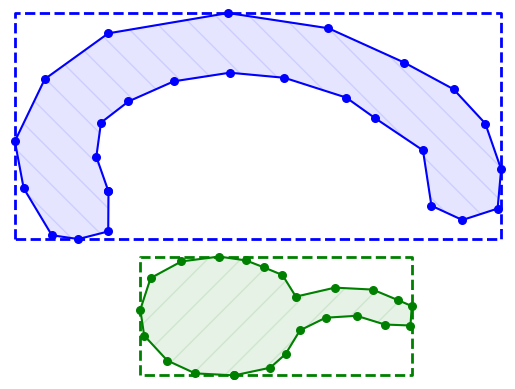
\includegraphics[width=4.25cm]{images/bbox_none.png} }}
    \qquad
    \subfloat[]{{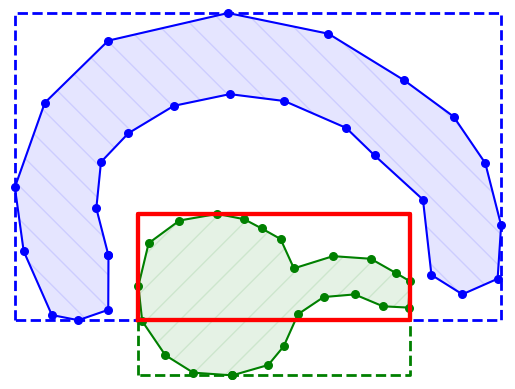
\includegraphics[width=4.25cm]{images/bbox_partial.png} }}%
    \qquad
    \subfloat[\label{fig:fully_contained_bb}]
    {{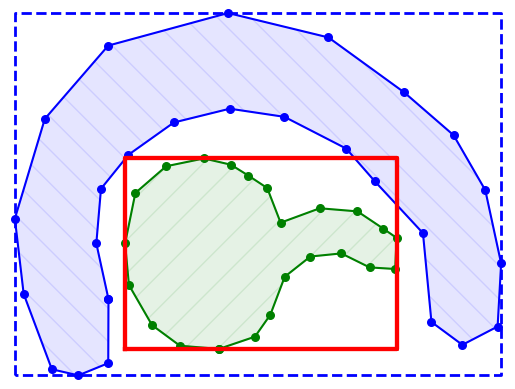
\includegraphics[width=4.25cm]{images/bbox_inside.png} }}%
    \caption{Possible intersection cases between bounding boxes. The common bounding box is in red. \textbf{(a)}: None, \textbf{(b)}: Partial, \textbf{(c)}: Contained.}
    \label{fig:bbi}
\end{figure}

The methods below are based on the assumption that, for the domain of maps, line segments of geometries should not self-intersect, and any occurrence of such is considered an error \cite{self_intersection}. Therefore, if there exists a crossing between any two line segments, it can be concluded that an intersection exists between the two different geometries.


\label{initialAlgo}
\subsection{Initial Intersection Algorithm}

The first algorithm to calculate the predicate intersection is presented below. The algorithm is constrained to not include line segments without an endpoint in the common bounding box and assumes that no shape is fully contained. Due to the constraints being violated in certain intersection contexts, the algorithm described in Section \ref{sect:chkintersect} is instead implemented in FPDE  to allow for more use cases.

\begin{figure}[htbp]
    \centering
    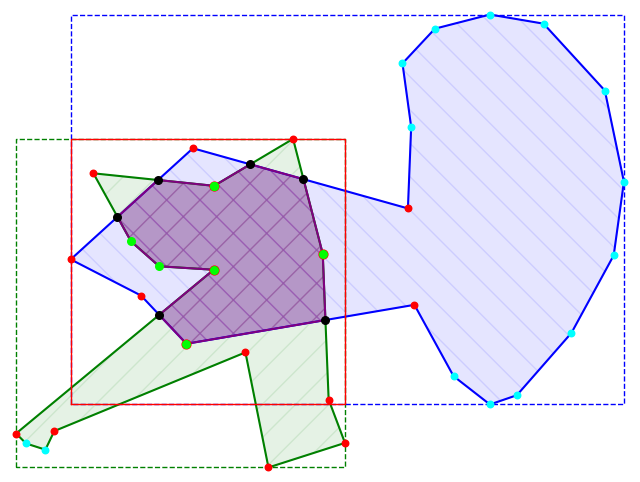
\includegraphics[width=8.5cm]{images/intersection_v1.png}
    \caption{Working case for the first intersection method. Green vertices are part of the intersecting shape, black are \textit{intersection points}, red are unnecessarily decompressed, and cyan are ignored.}
    \label{fig:intersectv1demo}
\end{figure}

When investigating two different geometries, the only area in which they can co-exist is inside the overlap of the bounding boxes. Consequently, an intersection between the two can only occur inside this overlap. The first method tries to avoid local decompression of points outside this area using the following steps:

\begin{enumerate}
    \item Check if the two geometries' bounding boxes overlap; if yes, continue to (2), else return False.
    \item Extract all the points within the overlap of the bounding boxes and add them to a set \textit{S}.
    \item Create a set \textit{L} of all line segments with an end point in \textit{S}.
    \item Check for intersections between any two line segments from each shape.
    \item  Return True if an intersection is found in (4), otherwise return False.
\end{enumerate}

Step (1) is trivially checked using the \textit{separating axis theorem}, while extracting all the points inside the overlap of the bounding boxes in (2) is more involved and requires additional data in the format header. One solution to finding the points is to store two sorted indices lists for the points based on their respective x- and y-value in the compressed format. Since an index can be saved with a maximum of $\lceil \log_2(n) \rceil$ bits, where $n$ is the total number of points in the geometry, the additional per-point overhead is relatively small. 

When the indices lists sorted by x- and y-values are accessible, the points inside the intersecting area of the bounding boxes can be found in $\mathcal{O}(\log_2(n)) \cdot T(random\_access)$ time using four binary searches over the sorted indices list for each geometry. The binary search finds the closest points to each of the bounding box overlap's perimeters; denoted as $x_{left},\ x_{right},\ y_{bottom},\ y_{top}$. When these points are found, the points with x-values between the range $(x_{left},\ x_{right})$ and $(y_{bottom},\ y_{top})$ can be extracted by slice indexing the sorted index lists and taking the set intersection. The last step in extracting all points within the area is to use random access, described in Section \ref{Random_access}, to get the actual points corresponding to the remaining indices.

Step (3) of the algorithm creates all line segments with the points found in (2) over the set of points in the bounding box overlap. Lastly (4) can utilize the \textit{sweep lines algorithm} to efficiently find any line segment intersection, as opposed to comparing each line segment of each geometry with each other.

Figure \ref{fig:intersectv1demo} demonstrates the algorithm. Only the vertices on a segment which is inside the common bounding box are decompressed, with some exceptions during the binary searches.

\begin{figure}[htbp]%
    \centering
    \subfloat[\centering The red intersection points are not found.]{{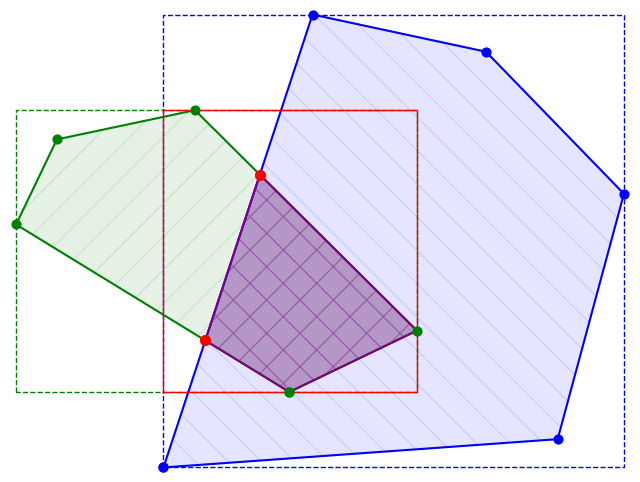
\includegraphics[width=6.9cm]{images/v1_fail_line.png} }}%
    \qquad
    \subfloat[\centering Intersection with no crossing line segments.]{{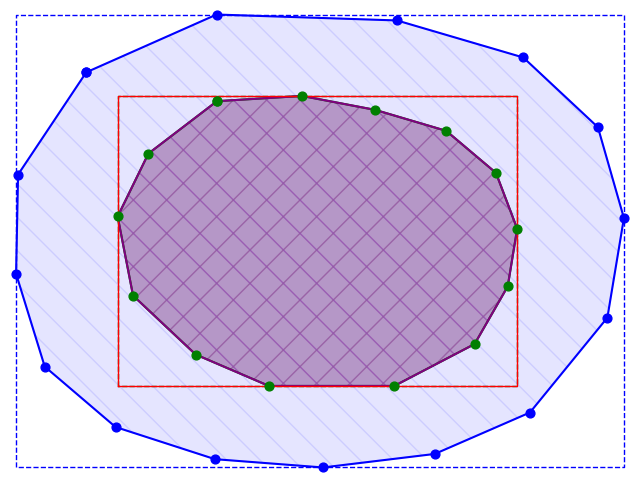
\includegraphics[width=6.9cm]{images/v1_fail_contains.png} }}%
    \caption{Example of failing cases for the first intersection method.}%
    \label{fig:bbFail1}%
\end{figure}

This algorithm works efficiently since it usually operates on a fraction of the geometries' points and line segments. However, it is limited in the sense that certain cases are not processed correctly. Since the algorithm is centralized around creating line segments with any endpoint inside the bounding box overlap, the algorithm does not consider line segments that cross the geometry bounding box overlap area but have both endpoints outside it. Another case in which the algorithm can fail is when the geometries' line segments never cross each other, but one is entirely contained in the other. Figure \ref{fig:bbFail1} shows an example of such cases. Due to these constraints, additional algorithms supporting more use cases for \textit{Is Intersection} and \textit{Intersection} are proposed below.





\subsection{Chunk Based Intersection}
%(Binärt) träd för att indexera baserat på plats. Plats -> index/offset
%Även hur vi lagar och parsear dessa på bästa sätt.  Behöver vi läsa in hela trädet?
\label{sect:chkintersect}
By utilizing the automatic chunking of FP-delta, the implementation for intersection can be improved further. Below, a method that uses the chunk's bounding boxes for reducing the size of the required local decompression is presented.
\\\\
Since the chunks contain a continuous sequence of points, the spatiality of the chunks is localized. As seen in Figure \ref{fig:chunks}, the bounding boxes of the chunks divide the geometry into a set of mostly non-intersecting rectangles. By examining the bounding boxes of the chunks, the relevant chunks which are within the common geometry bounding box can be extracted.

\begin{figure}[htbp]
    \centering
    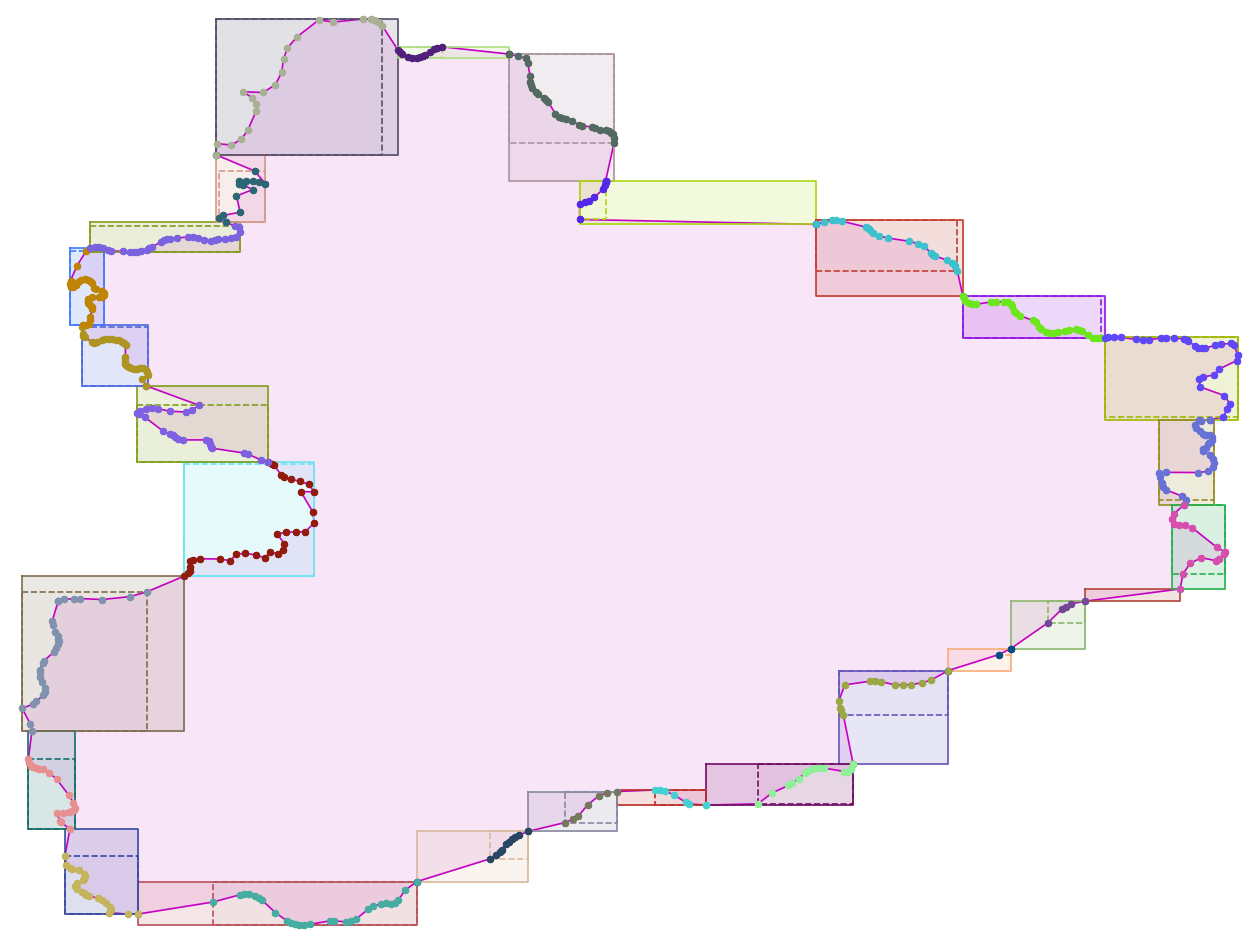
\includegraphics[width=10cm]{images/chunks.png}
    \caption{Bounding boxes of the chunks when including the first point in the following chunk. Dashed line is the bounding box if only containing the points within each chunk.}
    \label{fig:chunks}
\end{figure}

When all chunks within the bounding box have been found, additional filtering is applied to reduce the number of decompressed chunks. As outlined in Section \ref{initialAlgo}, the \textit{separating axis theorem} can be used to check if two bounding boxes overlap. This theorem is applied between the chunk-local bounding boxes between each of the geometries. If a chunk is found to have no bounding box overlap to any of the chunks from the other geometry, assuming no self-intersecting geometries, an intersection point can not exist on the segments in that chunk. For \textit{Is Intersection}, there is no meaning in decompressing such a chunk, but for \textit{Intersection}, it cannot be dismissed yet. In \textit{Intersection}, the segments in a chunk that does not have a bounding box overlap with any of the chunks in the other geometry might still be a part of the output polygon, as they may link the chunks containing intersecting segments. Due to this, these chunks are marked with mock segments and are lazily decompressed at a later stage when it is definite that its segments will be used.

Once the filtering has been completed, the chunks are decompressed and all points within them are used to form line segments. Each chunk forms one linestring consisting of the chunk's line segments. Furthermore, all linestrings filtered from geometry $g_1$ are checked for intersection with all linestrings filtered from  geometry $g_2$. This procedure results in a set $S$ that contains the intersecting points. If $S \neq \emptyset$ then there exists an intersection between the shapes, otherwise additional steps are required to determine the intersection status.

\subsubsection{Fully Contained}
\label{sec:fully_contained}
As stated in the previous algorithm, when one shape is fully contained within the other, there is an intersection between the shapes, even though there are no intersecting points between the shape's line segments. By looking at the relationship between the shapes' global bounding boxes, it can be determined whether it is possible for one shape to be fully contained within the other. Namely, in order for a shape to be fully contained, its bounding box must also be fully contained within the other shape's bounding box. The reason for this is that since the shapes are contiguous (if not dealing with multipolygons), there must exist a path between the points spanning the bounding box. This path will be outside the bounding box of the other shape, and since the geometry is at least as small as its bounding box it can be concluded that the shape cannot be fully contained.

\begin{figure}[htb]
    \centering
    \includegraphics[width=10.75cm]{images/intersecting_ray.png}
    \caption{A query where a ray, visible as the dotted red line, is used to determine intersection. Only the chunks in black (red and green points) are decompressed for the complete query.}
    \label{fig:intray}
\end{figure}

\label{sec:pointinshape}
However, if the bounding box $bounds(g_1)$ is fully contained in $bounds(g_2)$, further evaluation is needed. Since there are no point intersections, the whole geometry is either inside the other shape, or completely outside (but still within its bounding box), as in Figure \ref{fig:fully_contained_bb}. The \emph{crossings test} can be used to determine whether a point is within a shape \cite{polygonalgos}. The test works by sending a ray from the point along an axis, and counting the number of crosses over the shape. If the number is odd, then the point is within the shape, otherwise outside. By picking a random vertex from $g_1$ and performing the crossings test between the vertex and $g_2$, it can be determined that if the point is inside $g_2$, then $g_1$ is fully contained within $g_2$ and $g_1$ is the resulting intersecting shape. An example of an intersection query where the test is performed can be seen in Figure \ref{fig:intray}.


Implementation wise, the ray test in FPDE is implemented by constructing a linestring between the point and the other shape's bounding box. The direction is chosen such as to minimize the length of the line segment. The above steps for finding the intersecting points are then executed for $g_2$ with the common bounding box being the linestring. The number of intersecting points is then equal to the number of crossings.

\begin{figure}[htb]
    \centering
    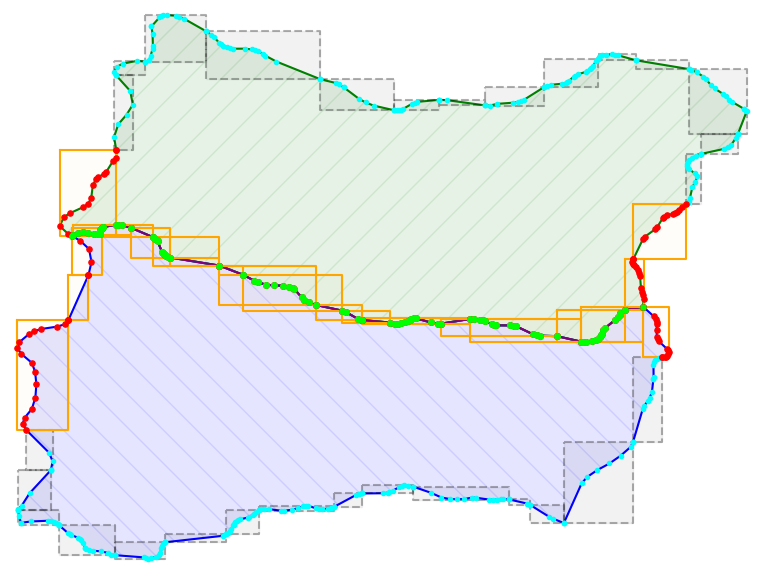
\includegraphics[width=13cm]{images/intersection_world.png}
    \caption{One example from the \emph{Admin Borders} dataset. Only the chunks in black (red and green points) are decompressed. Green vertices are part of the intersecting shape, red vertices are unnecessarily decompressed, and cyan vertices are ignored. }
    \label{fig:intworld}
\end{figure}

As seen in Figure \ref{fig:intworld}, the algorithm has the benefits of local decompression being restricted to the chunks that overlap between the geometries and that are within the common bounding box, with the possible exception of chunks that cross the ray used to test for fully contained shapes. But it also has drawbacks, such as requiring the bounding boxes of the chunks to be quickly accessible and that all points within the overlapping chunks are decompressed.

\starsubsection{Quadtrees for Chunk Based Spatial Indexing}
\label{sec:quadtreechunk}
This section introduces a storage-efficient alternative to spatially indexing chunks. Due to time constraints, implementing the indexing is left as future work.

The overhead for the method presented above comes from the need to find all the chunks possibly involved in an intersection. In the FPDE implementation, all chunks' bounding boxes are stored as full coordinates, adding an additional four floating-point coordinates per chunk to the compressed file, and finding the relevant chunks is done through a linear search. 

Section \ref{sec:quadtreeapproximation} describes how the chunks' bounding boxes can be approximated by utilizing a quadtree. With this approach, the bounding boxes of the chunks are essentially snapped to the smallest quadrant in the quadtree in which they are fully contained.

\begin{figure}[htbp]%
    \centering
    \subfloat[\centering Chunks belong to the smallest quadrant in which they are fully contained.]{{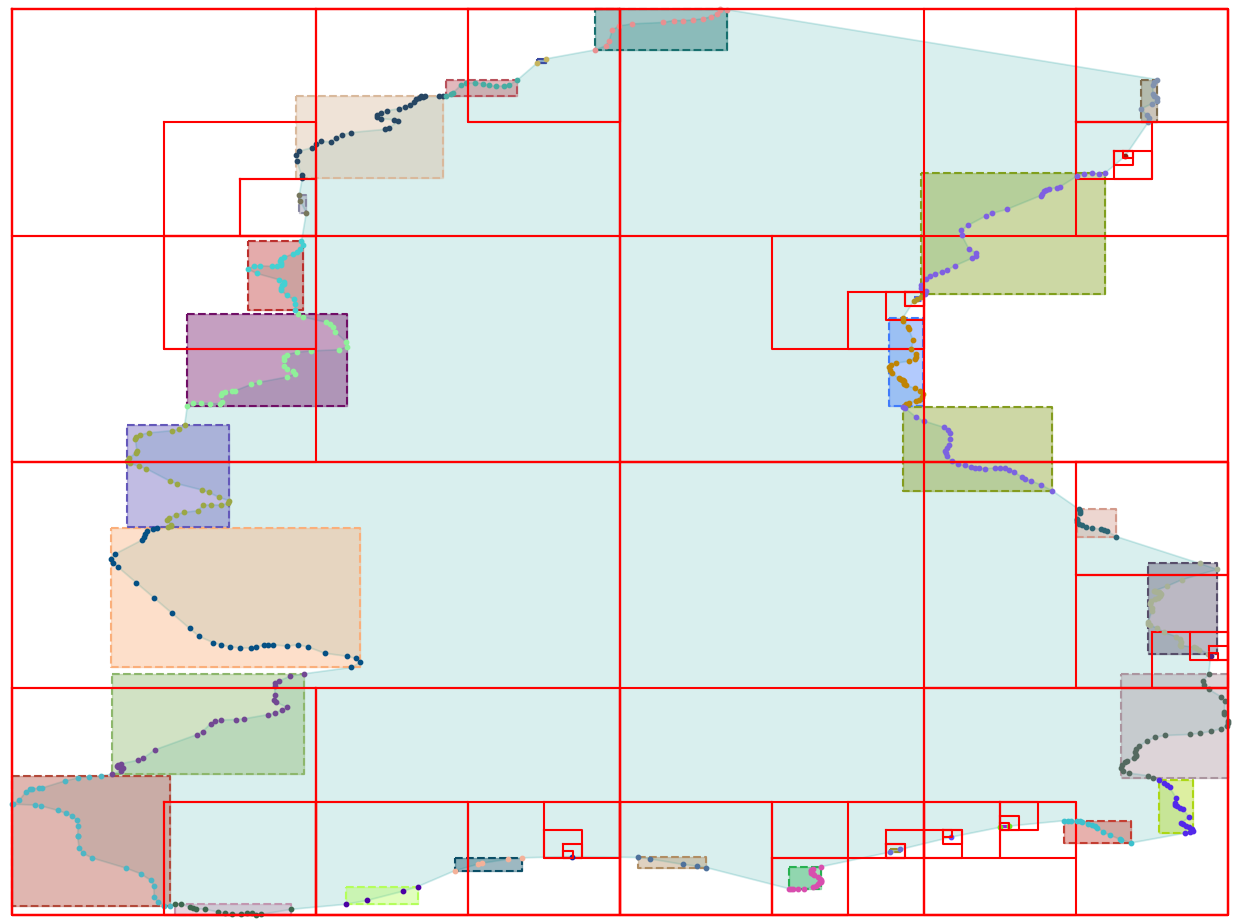
\includegraphics[width=6.9cm]{images/quadtree_contained.png} }}%
    \qquad
    \subfloat[\centering Chunks can belong to multiple quads.]{{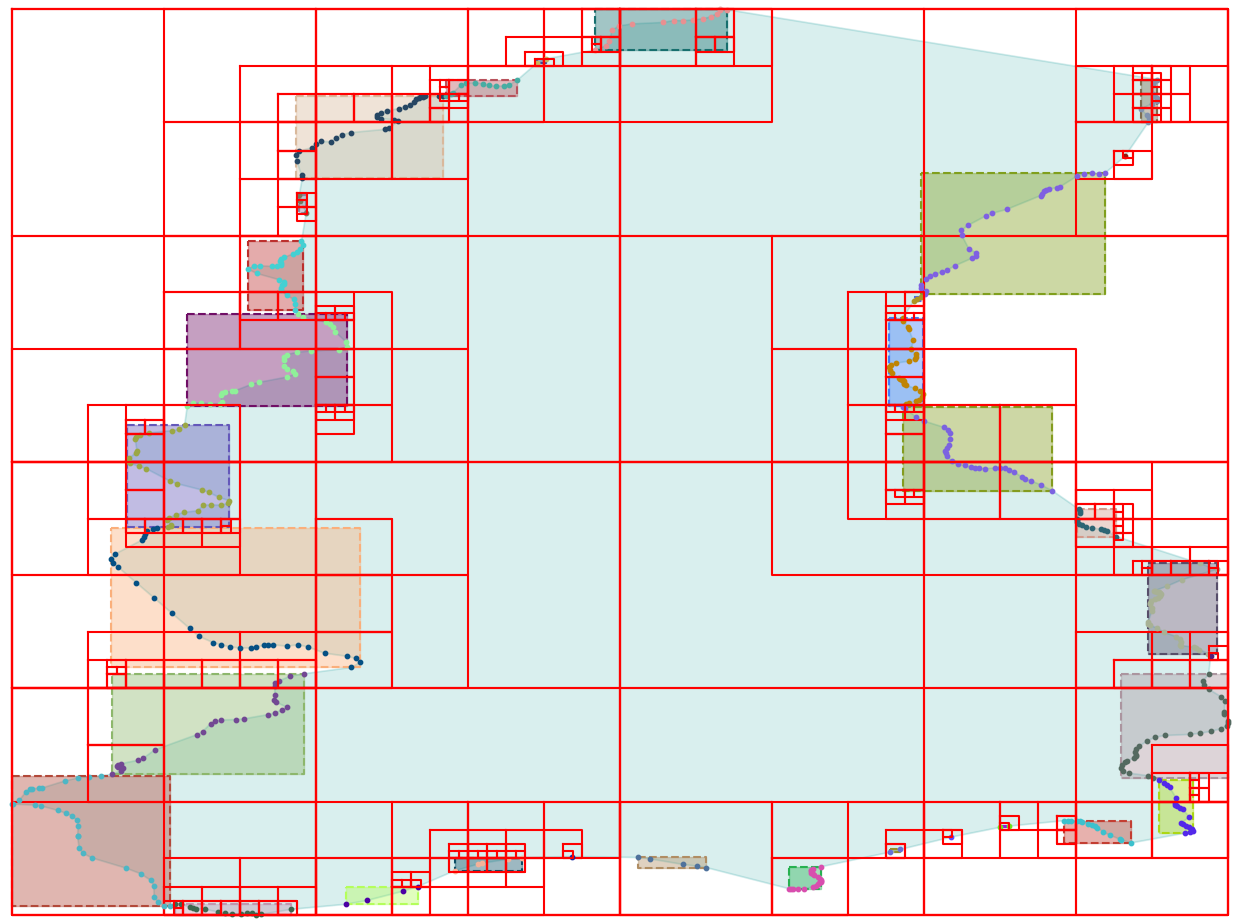
\includegraphics[width=6.9cm]{images/quadtree_min.png} }}%
    \caption{Two configurations of using quadtrees to spatially index chunks.}%
    \label{fig:chkbboxquad}%
\end{figure}

As seen in Figure \ref{fig:chkbboxquad}(a), the quadtree introduces a hierarchy of bounding boxes. The hierarchy allows for a reduction in storage overhead since encoding the bounds of the chunks is done through the tree structure, and the tree structure likely requires less storage space as opposed to storing the coordinates in full. Using a quadtree makes it possible to calculate the bounds of the chunks based on the shape's global bounding box and the position of the quadrants containing the chunks.

Furthermore, since the tree is hierarchically structured, intersection-filtering can be performed on multiple zoom levels. The quadtree can either be based on the geometry's bounding box or on a \emph{global grid}. In both cases, the traversal of the nodes in geometry $g_1$ can be stopped early if a quadrant in $g_1$ only intersects with leaf nodes without chunks in geometry $g_2$. Since if all the intersecting quadrants from $g_2$ are empty leaf nodes, there can be no chunks in those quadrants, and thus no line segments can possibly intersect between the shapes in $g_1$'s quadrant. Expanding the quadrant's subtree further is unnecessary.

% In terms of space, the required size to store the chunks $C$ in a quadtree with nodes $Q$ is:
% \begin{equation}
%     S = 4 \cdot \#(Q) + \#(C) \cdot len(\#(C)) = 4 \cdot \#(Q) + \#(C) \cdot \left \lceil{\log_2{(\#(C))}}\right \rceil 
% \end{equation}


One problem with assigning each chunk to one quadrant only is that the approximation errors may be big. As seen in Figure \ref{fig:chkbboxquad}, allowing chunks to be part of multiple quads results in a more detailed tree. However, this comes at the expense of storing more nodes.

\subsection{Constructing the Intersecting Shape}
Implementing the intersection operation which returns the resulting shape is an involved task, largely due to the numerous possible combinations of shapes and corner cases. The method presented below is an adaptation of the \emph{Weiler Atherton} and \emph{Greiner–Hormann} polygon clipping algorithms, extended to work with spatially separated chunking and linestrings.

\begin{figure}[htbp]
    \centering
    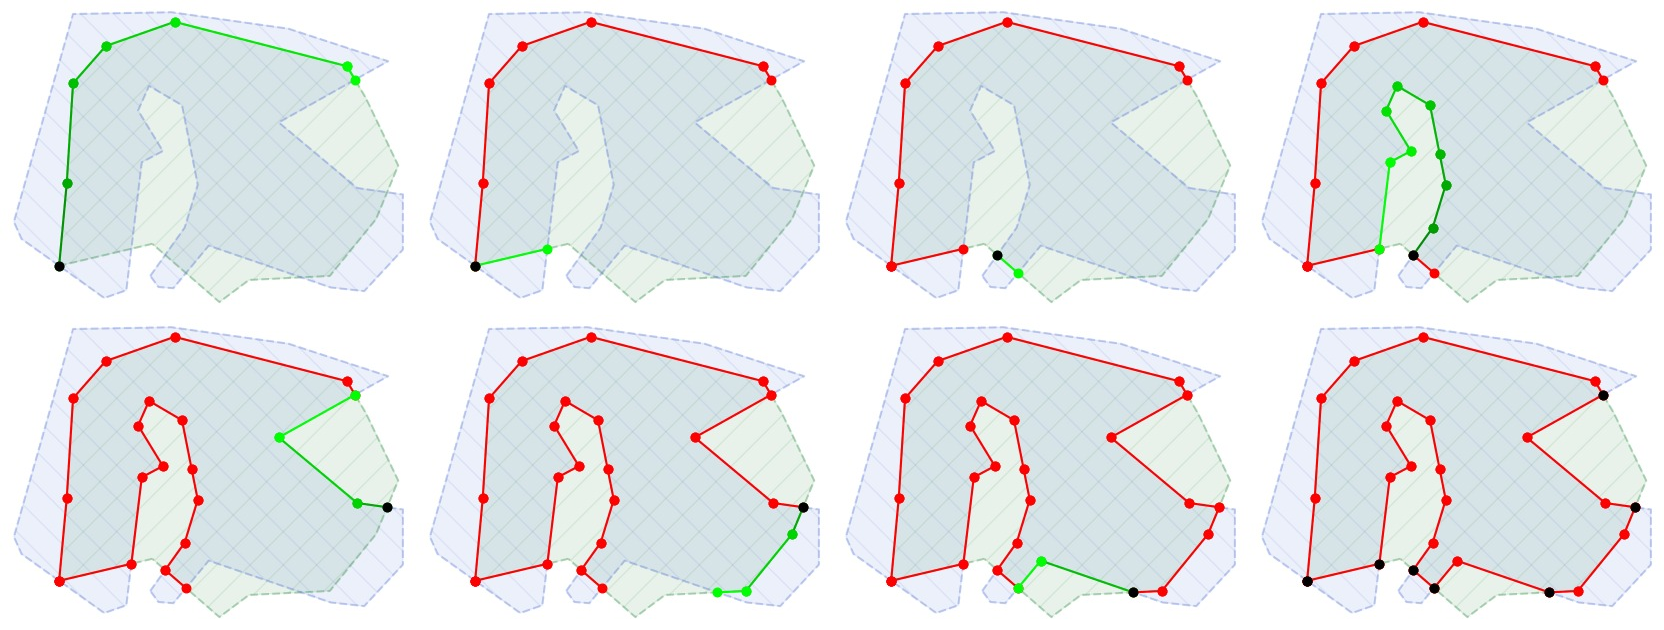
\includegraphics[width=15cm]{images/intersecting_shape.png}
    \caption{Finding the intersecting shape illustrated. Black vertex is the current \emph{intersection point}, green is the current path (traversing from dark to light), and red is the resulting shape.}
    \label{fig:shapegen}
\end{figure}

The steps for the implemented algorithm are the following (illustrated in Figure \ref{fig:shapegen}):
\begin{enumerate}
    \item The common bounding box is calculated. If no common bounding box exists, then the resulting shape is the None-shape. Otherwise, all chunks inside the common bounding box are found.

    \item Chunks with a bounding box that overlaps any of the chunks of the other geometry are immediately decompressed, while the rest are subject to lazy decompression.
   
    \item All segments within each decompressed chunk are merged into a linestring. The linestrings of overlapping chunks are pairwise, one from each shape, checked for intersection. Two dictionaries are created, one that enables finding all segments which cross a given intersection point, while the other is used to go in the other direction, i.e., retrieving all intersecting points which lie on a segment.

    \item Create a set $S = \{ intersecting\ points \}$. One intersection point $c_i$ is removed from $S$ and the valid edges from $c_i$ are traversed and added to the resulting shape. The traversal is stopped when encountering another intersection point. The procedure is repeated until $S = \emptyset$.

    This step can be implemented by first calculating the possible paths from $c_i$. At most four possible paths can exist since it is assumed that holes do not lie on the polygon border, and that there are no self-intersecting shapes. The paths are, for both shapes, traversed in both directions originating from $c_i$. Since at most two of the four paths are valid, the invalid paths are removed by verifying that the midpoint of the paths' first segment is within both shapes, using the \emph{crossings test} as explained in Section \ref{sec:pointinshape}. By traversing both directions, it is ensured that if the resulting shape is a linestring, that is, if no closed path is formed, then both ends are discovered.

    When the resulting shape is a polygon, both traversal directions can reach all points, and thus two paths can share the same edge. To avoid unnecessary calculations and duplicate segments in the final shape, it is also verified that the first segment in the path has not yet been visited.

    \item As explained for the predicate operation in Section \ref{sec:pointinshape}, intersection can occur even though there exist no intersecting points between the linestrings. In that case, the contained shape is returned.
\end{enumerate}

When verifying the paths, it is also verified that no two paths from one $c_i$ are parallel. This is done to avoid adding identical segments when two shapes share an edge.


%https://books.google.se/books?hl=sv&lr=&id=CCqzMm_-WucC&oi=fnd&pg=PA24&dq=shape+check+if+point+is+inside&ots=mvns05NIbe&sig=xaJJmCNMv9oP6BG4n14shw6zi1A&redir_esc=y#v=onepage&q=shape%20check%20if%20point%20is%20inside&f=false


% Bounding Boxes för chunks
% Läsa de chunks som är aktuella (undvik andra) i den gemensamma bounding boxen
% Packa upp dessa för finare evaluering
% Specialfall fully contained: skicka stråle
% C^2 jämför varje chunk med varje chunk
% Potentiell improvement med quadtree




% As mentioned above, geometries do not self-intersect, and any line segment crossing implies that the two geometries containing those line segments intersect. Looking at two geometries the only area they can possibly co-exist is the overlap of the bounding boxes which also implies any co-existing of line segments. Therefore intersection of two geometries can only occur inside this overlap.


% The first method for \textit{IsIntersection} tries to extract every point inside the area where line segment crossing can occur. Since the overlap of the bounding boxes is the only area where the two geometries can co-exist, an initial attempt is to extract all the line segments between points inside that area and their neighbours.

% Referring to \ref{fig:bbi}\textbf{(b)}, it can trivially be concluded that such intersecting line segments can only occur in the overlap of the geometries' bounding boxes and 


% The method for intersection Since we want to locally decompress as little information as possible, one intuitive method to check for intersection is to only use points inside the overlap of the geometries bounding boxes
% Now when the more interesting points, as seen in \ref{fig:bb}\textbf{(b)} are extracted, and local decompression has been done on those, the two operations \textit{IsIntersecting} and \textit{Intersection} take different routes. 




% For the domain of maps, line segments of geometries should not self-intersect, and any occurrence of such is considered an error \todo{källa}. With that assumption in mind, any pair of line segments from different geometries intersecting means that one geometry enters the interior part of the other. \todo{Nämna hur man kan använda line sweeps, bör skivas om i teorin innan} For \textit{IsIntersecting}, any occurrence of such line segment crossing leads to a return value of \textit{True}, representing that an intersection does occur. If no such pair exists, the conclusion can be drawn that an intersection does not occur. 
%FRÅGAN ÄR OM MAN SKA BÖRJA SKRIVA OM FPDE detaljerad implementaion med binary search och hur vi sparar sorterade listor redan här. Även lite osäker om du tänkte att denna mer detaljerade delen skulle vara här, men tänkte att det oavsett kommer behöva skriva någon gång



\section{Optimizing the Compression Ratio}
In this section, additional ideas and implementations that extend FPDE to improve the compression ratio are discussed. First, the alternatives between different formats for representing the coordinates are presented, followed by entropy encoding of the deltas.

\subsection{Floating-Point Coordinate Representation}
\label{sec:delta_mod}
As described in Section \ref{section:fpd}, the standardized way to represent floating-point values is according to the IEEE 754 standard. The standard supports either 32 or 64-bit precision, where high-precision coordinate values can be stored losslessly using the latter, as in the WKB format. Maps data may consist of coordinates with a precision below the need for 64-bit double precision. When this is the case, reducing the number of bits used to represent the floats will decrease the overall size of the geometry format. Two floating-point coordinate representations specific to maps data are presented below.

\subsubsection{Variable Precision Float}
\begin{figure}[htbp]
    \centering
    \includesvg[width=13cm]{images/varfloat.svg}
    \caption{Structure of the \textit{variable precision float} format with a minimal exponent allowing an integer part between \(\pm 180\).}
    \label{img:variable_precision}
\end{figure}

The structure for representing floating-point values proposed in Figure \ref{img:variable_precision} is a modification of the IEEE 754 standard, with a variable exponent and mantissa size. The perk of having variable exponent and mantissa bit-lengths is that it allows for domain-specific optimizations.

For instance, the standard exponent size of IEEE 754 with 64-bit precision allows values ranging between $\pm 9\ 007\ 199\ 254\ 740\ 992$. While for the domain of maps, coordinates are within the range of $\pm 180$, so there is no need to use an exponent part that allows integer ranges outside of that. Therefore, it makes sense to either remove those bits to lower the format size or dedicate some of the unnecessary exponent bits to the mantissa part for a higher floating-point precision.

OpenStreetMap data coordinates use at maximum seven decimal points. Therefore, using the \textit{variable precision float} format with a 4-bit exponent and 32-bit mantissa is enough to represent all coordinates for such data, resulting in a decrease of 27 bits per coordinate from the original 64-bit representation. If full double precision is required, the decrease of bits in the exponent part reduces the total size by 7 bits.


\subsubsection{32-Bit Integer Decomposed Coordinate}
\label{32-bit}
An alternative format that also takes advantage of the limited range of the integer part of the floating-point values in the domain of geographic coordinates is \textit{32-bit integer decomposed coordinate}, illustrated in Figure \ref{img:intdecompflow}. The encoding of the format is performed by adding 180 to the floating-point value, to convert the coordinate to the positive space, followed by concatenating the integer and decimal part into one large unsigned integer value. The integer value is then converted to its corresponding bit sequence.

\begin{figure}[htbp]
    \begin{adjustwidth}{15pt}{}
        \includesvg[width = 400pt]{images/int_decomp.svg}
    \end{adjustwidth}

    \caption{Illustration of converting from floating-point value to a 32-bit integer decomposed coordinate sequence.}
    
    \label{img:intdecompflow}
\end{figure}

The latitude and longitude values of geographic coordinates range between \(\pm 90\) and \(\pm 180 \), respectively \cite{dec_deg}. Thus, the number of possible values for the longitude, when using \(X\) decimals of precision, is \(2 \cdot 180 \cdot 10^{X}\). This is strictly greater than the amount of possible combinations of latitude values with the same decimal precision. For this expression to fit in a 32-bit integer, the precision of the coordinate can not transcend seven decimal points, or else they need to be truncated in a compression-lossy manner. However, since the seventh longitude decimal point corresponds to a real-time accuracy of 1.11 cm at the equator and an even higher accuracy when deviating from it \cite{dec_deg}, the loss of precision above this limitation may be considered acceptable. For instance, as previously noted, OSM operates on coordinate points with up to seven decimal points of precision \cite{osm_precision}, which supports the adequacy of the format for general-purpose mapping applications.
\\\\
When calculating the deltas for coordinates in the IEEE 754 format, only the exponent and sign parts are usually similar between the bit sequences of two adjacent values. Consequently, only those bits systematically cancel out. The mantissa, which covers a great fraction of the bits in IEEE 754, is still generally significantly different.

By using 32-bit integer decomposed coordinates instead, the number of leading zeros in the zigzag encoded deltas is inversely proportional to the distance between the coordinates, and hence the deltas have the possibility of being significantly smaller. However, it is worth recalling that using 32-bit integer decomposed coordinates is not as general as using the IEEE 754 format, as the coordinates are limited to seven decimal points.


\subsection{Entropy Encoding of Deltas}
When using delta encoding, a distribution of the different delta values emerges. If the distribution is not uniform, there is an indication of possible entropy encoding, where more frequent deltas are encoded with fewer bits than infrequent ones. This section presents how Huffman and Golomb-Rice encoding, explained in Section \ref{section:huff}, can be applied to the deltas in the format. %In figure \ref{img:entropy}, it can be seen, intuitively, how the deltas can create a distribution of values.

% \begin{figure}[H]
%     \begin{adjustwidth}{20pt}{}
%         \includesvg[width = 400pt]{images/entropy distribution.svg}
%     \end{adjustwidth}

%     \caption{An illustration how delta values create a distribution which can be entropy encoded}
%     \label{img:entropy}
% \end{figure}

\subsubsection{Huffman Encoding}
Huffman encoding maps a symbol to a bit sequence, and in the context of FPDE each zigzag encoded delta is a symbol.

One way to create a Huffman encoding tree is to use the frequencies of the delta symbols over all geometries in a dataset. However, if the Huffman encoding tree is based on multiple geometries with different delta bit-lengths, a suboptimal Huffman tree will be created since the character space contains deltas of all the combined bit-lengths. 

Instead, as the geometries in FPDE have different but fixed delta bit-lengths, a more efficient approach is to construct a set of smaller Huffman trees, each built with deltas of equal bit-length. This strategy avoids using a Huffman tree where certain values cannot occur because of the fixed delta bit-lengths of the geometries. Furthermore, the frequency distribution of the deltas may vary depending on the specific bit-length involved.

\subsubsection{Golomb-Rice Encoding}
Similarly to Huffman encoding, Golomb-Rice encoding can be used to decrease the size of the delta values. As for Huffman encoding, the possible delta values are used as symbols in the encoding. Golomb-Rice encoding performs particularly well when the delta values are clustered around small values and if the frequency decay follows a geometric distribution.

The advantage of Golomb-Rice encoding compared to Huffman encoding is that the overhead is lower. While Golomb-Rice encoding only requires the parameter $k$ to be saved, Huffman encoding requires the entire Huffman tree to be stored, either locally in the geometries or globally as a library variable. 

A suitable value for the parameter $k$ can be calculated using Equation \ref{eq:rice_form}. 


% \todo{lägg till pred functions efter redovisning}
%\subsection{Predictor Functions}
%which use the surrounding context to estimate the deltas.
\chapter{Results}
In this chapter, the results for our implementation and the baseline are presented for various configurations. Compression time and execution time for the operations are presented, along with the achieved compression factor. 

The datasets used for the evaluation are described in Section \ref{sec:datasets} and consist of: \emph{Sweden Buildings}, \textit{Sweden Roads}, \textit{Sweden All}, \textit{China Water}, and \textit{Admin Borders}. For intersection, a subset of \textit{Sweden All}, combined with \textit{China Water}, and \textit{Admin Borders} are used.

The computer used to benchmark was a MacBook Pro 2018 with a 2.9 GHz 6-Core Intel Core i9 processor and 32 GB 2400 MHz DDR4 RAM.

\section{Compression Factor \& Overhead}

In the following section, the compression factor is discussed with regard to various settings for the dataset and algorithm used. The compression factors are presented in Figure \ref{fig:compfactorres} and Table \ref{tab:compsize_tab}. When a limit is enforced on the number of deltas within a chunk to support faster random access, a maximum chunk length of 13 deltas is used. Furthermore, due to its widespread application in the industry, WKB is used as a reference for comparing the size of various configurations.
\\\\
The configurations used for the algorithm are described below and summarized in Table \ref{tab:comp_config}:

\begin{description}
     \item [WKB (Uncompressed)] Well-known binary to represent the shapes.
     
    \item [FPD] 64-bit floating-point delta encoding without support for efficient operations.

    \item [FPDE] The implementation referenced throughout the thesis. Consists of 32-bit integer decomposed coordinates and extensive metadata to allow efficient operations.
    
    \item [FPDE: Arbitrary Precision] FPDE using 64-bit floating-point delta encoding, i.e., the default encoding if not using 32-bit integer decomposed coordinates. The configuration has efficient support for operations.

    \item [FPDE: Entropy Encoding] FPDE with entropy encoding for the deltas. Each geometry is assigned the most size efficient entropy encoding method; either Huffman encoding, Golomb-Rice encoding or no entropy encoding.

    \item [FPDE: Size Optimized] FPDE using 32-bit integer decomposed coordinates, without any extra metadata for the operations. No limit on the number of deltas per chunk and entropy encoding is applied without the size overhead, which disables random access.

    \item [WKB: gzip] WKB, followed by \textit{gzip} compression.
    
    \item [WKB: bzip2] WKB, followed by \textit{bzip2} compression.
\end{description}

\begin{table}[h]
\centering
{\setlength{\extrarowheight}{5pt}%
\resizebox{\textwidth}{!}{%
\begin{tabular}{|l|l|l|l|l|}
\hline
\textbf{\begin{tabular}[c]{@{}l@{}}Compression \\ Method\end{tabular}} & \textbf{\begin{tabular}[c]{@{}l@{}}Floating-Point\\ Encoding Scheme\end{tabular}} & \textbf{\begin{tabular}[c]{@{}l@{}}Support for \\ Operations\end{tabular}} & \textbf{\begin{tabular}[c]{@{}l@{}}Max Chunk\\ Length\end{tabular}} & \textbf{\begin{tabular}[c]{@{}l@{}}Entropy \\Encoding\end{tabular}} \\ \hline
WKB (Uncompressed)                                                     & 64-bit IEEE 754                                                                   & \ding{51}                                                                        & -                                                                      & \ding{53}                                                                            \\ \hline
FPD                                                         & 64-bit IEEE 754                                                                   & \ding{53}                                                                         & \ding{53}                                                                     & \ding{53}                                                                            \\ \hline
FPDE: Arbitrary Precision                                               & 64-bit IEEE 754                                                                   & \ding{51}                                                                        & \ding{51}                                                                     & \ding{53}                                                                            \\ \hline
FPDE                                                                   & \begin{tabular}[c]{@{}l@{}}32-bit integer \\ decomposed coordinates\end{tabular}    & \ding{51}                                                                        & \ding{51}                                                                    & \ding{53}                                                                            \\ \hline
FPDE: Entropy Encoding                                                 & \begin{tabular}[c]{@{}l@{}}32-bit integer  \\ decomposed coordinates\end{tabular}    & \ding{51}                                                                        & \ding{51}                                                                    & \ding{51}                                                                           \\ \hline
FPDE: Size Optimized                                                   & \begin{tabular}[c]{@{}l@{}}32-bit integer \\ decomposed coordinates\end{tabular}    & \ding{53}                                                                        & \ding{53}                                                                     & \ding{51}                                                                           \\ \hline
WKB: gzip                                                              & 64-bit IEEE 754                                                                   & \ding{53}                                                                         & -                                                                      & \ding{51}                                                                            \\ \hline
WKB: bzip2                                                             & 64-bit IEEE 754                                                                   & \ding{53}                                                                         & -                                                                      & \ding{51}                                                                            \\ \hline
\end{tabular}}}
\caption{The methods used for compression with their respective configurations summarized.}
\label{tab:comp_config}
\end{table}

\begin{figure}[htbp]
    \centering
    \includesvg[width=12.0cm]{images/comp_factor.svg}
    \caption{Compression factor for various configurations. 30 000 random samples from each dataset were used. Average of all shape's factors. WKB is used as the uncompressed representation and the factor is thus in relation to WKB.}
    \label{fig:compfactorres}
\end{figure}


\begin{table}[htbp]
\centering
\caption{Compression factor and ratio (\%) when calculated over all samples, i.e., the combined size of all shapes in WKB representation divided by the combined compressed size.}
%\begin{adjustwidth}{-1cm}{}
\resizebox{\textwidth}{!}{%
\begin{tabular}[h]{l|ccccccccc}
\toprule
Dataset & WKB & FPD & Arbitrary & FPDE & Entropy & Size Opt & WKB: gzip & WKB: bzip2 \\
\midrule 
Sweden Buildings & 1.0 (100) & 1.85 (54) & 0.88 (113) & 1.82 (54) & 1.8 (55) & 4.45 (22) & 0.75 (133) & 1.07 (93) \\
Sweden Roads & 1.0 (100) & 1.57 (63) & 0.95 (105) & 2.11 (47) & 2.11 (47) & 4.22 (23) & 0.79 (126) & 1.05 (95) \\
Sweden All & 1.0 (100) & 1.65 (60) & 1.04 (96) & 2.34 (42) & 2.39 (41) & 4.64 (21) & 0.92 (108) & 1.2 (83) \\
China Water & 1.0 (100) & 1.67 (59) & 1.2 (83) & 2.78 (35) & 2.85 (35) & 4.73 (21) & 1.09 (91) & 1.31 (76) \\
Admin Borders & 1.0 (100) & 1.39 (71) & 1.07 (93) & 2.21 (45) & 2.64 (37) & 4.22 (23) & 1.18 (84) & 1.3 (76) \\
\midrule
Average & 1.0 (100) & 1.62 (61) & 1.03 (97) & 2.25 (44) & 2.56 (39) & 4.45 (22) & 0.95 (105) & 1.18 (84) \\ 
\bottomrule
\end{tabular}}
%\end{adjustwidth}
\label{tab:compsize_tab}
\end{table}





Figure \ref{fig:compfactorres} and Table \ref{tab:compsize_tab} show that the compression factor is affected by the compression algorithm used and the attributes of the datasets. The order of the algorithms with the highest compression factors remains consistent across the various datasets, where the general-purpose algorithms perform the worst, and FPDE with disabled partial decompression performs the best. As shown in the same figure, some configurations generally perform better on certain datasets than others. In the following section, a comparison between the results for the different algorithm variations is presented, followed by an analysis of the effects that the attributes of the datasets have on the compression ratio.

\subsubsection{Algorithm Comparison}
According to Table \ref{tab:compsize_tab}, the order of the average compression performance is: \textit{WKB: gzip}, \textit{WKB}, \textit{FPDE: Arbitrary Precision}, \textit{WKB: bzip2}, \textit{FPD}, \textit{FPDE}, \textit{FPDE: Entropy Encoding}, followed by \textit{FPDE: Size Optimized}. The general-purpose algorithms are expected to perform the worst, as they do not exploit domain-specific structures and are based on general ideas. When comparing the performance between the FPDE configurations, they seem to be ordered by the format of the floating-point coordinates, the overhead of supporting optimized operations, and whether entropy encoding is utilized or not. 

\begin{figure}[htbp]
    \centering
    \includesvg[width=15cm]{images/overhead_distr.svg}
    \caption{The total size distribution within average geometries from the datasets using FPDE. \textit{Chunk BBs} is the overhead of the bounding boxes of the chunks, required by the optimized intersection operation. A maximum chunk length of 13 deltas and no entropy encoding was applied. 100 000 random samples were used.}
    \label{fig:overheaddistrb}
\end{figure}

The distribution of various components in FPDE is visualized in Figure \ref{fig:overheaddistrb}, where it can be seen that the overhead of the operations in FPDE occupies a significant amount of space. This is the main reason why \textit{FPDE: Size Optimal} yields superior compression compared to \textit{FPDE}, along with the utilization of entropy encoding. Additionally, since \textit{FPDE: Size Optimal} does not require additional overhead to support operations with entropy encoded deltas, the format gains the full effect of entropy encoding, shown in Table \ref{tab:entropyDeltas}. On the contrary, when comparing \textit{FPDE: Entropy Encoding} to \textit{FPDE} in Table \ref{tab:compsize_tab}, it is discovered that the extra overhead, which allows the former to perform operations with entropy encoded deltas, offsets the gains of the entropy encoding.

Another observation is the effect of using different formats for representing the geometry coordinates, where algorithms that utilize 32-bit integer decomposed coordinates outperform those using 64-bit IEEE 754 floating-point coordinates. However, while the effect is self-evident, using the former comes at the cost of its coordinate precision constraint of 7 decimals, as outlined in Section \ref{32-bit}. Additionally, it is essential to note that for configurations that use 32-bit  coordinates, the compression factor is directly increased, due to the halving of the bit representation from 64 to 32 bits.  Thus, in those cases, if operation speed is lacking and the compression factor is close to the effect of just changing the floating-point representation, it would be unnecessary to utilize the integrated operation support. Instead, it might be beneficial to store the geometries directly using the 32-bit format without additional compression, and run the operations directly to avoid the extra decompression overhead. Therefore, to representatively compare the effect caused by the induction of operability on the compression ratio, the algorithm configurations that use the same coordinate format should be compared, such as \emph{FPD} versus \emph{FPDE: Arbitrary} and \emph{FPDE: Size Optimized} versus \emph{FPDE: Entropy Encoding}. As evident by Figure \ref{fig:overheaddistrb}, the operation overhead represents a significant portion of the data, resulting in a decreased compression ratio. However, it is worth noting that the overhead varies greatly on a per-shape basis, and that the overhead of the chunk bounding boxes likely can be significantly reduced in future work by, for example, using a quadtree.

\subsubsection{Influence of Dataset Attributes}
As evident by Figure \ref{fig:overheaddistrb}, the distribution between various components in FPDE varies heavily between the datasets. Alongside the \textit{$\mathrel\#$ Vertices} column in Table \ref{tab:chunks}, it is apparent that there is a correlation between the number of vertices in the geometries and the proportion of deltas in its compressed form. As deltas are the essence of compression, they contribute to an increased compression factor. The reason for the increase in proportion of deltas is that with more complex shapes, the overhead of the global bounding box data diminishes in relation to the coordinate data. Additionally, as seen in Table \ref{tab:chunks}, the average number of vertices in each chunk is higher for datasets with a higher vertex count, causing more deltas in relation to coordinates represented in full. 

\begin{table}[htbp]
\centering
\caption{Chunking statistics based on an average of 100 000 random samples with a maximum chunk size of 13 deltas.} 


\label{tab:dataset_stats_chunking}
%\begin{adjustwidth}{-1.3cm}{}
\resizebox{\textwidth}{!}{%

\begin{tabular}{@{\extracolsep{4pt}}lcccccc}
\toprule   
 {} & {} & {} & {} & \multicolumn{3}{c}{$\mathrel\#$ Vertices in Chunks}\\
 \cmidrule{5-7}
Dataset & $\mathrel\#$ Vertices & Delta Bit Size & $\mathrel\#$ Chunks & Average & Standard Deviation & Median \\ 
\midrule
Sweden Buildings & 6.3 & 12.3 & 1.0 & 5.0 & 0.1 & 5.0 \\ 
Sweden Roads & 12.7 & 13.7 & 1.6 & 6.5 & 1.0 & 6.7 \\
Sweden All & 16.3 & 13.2 & 1.9 & 6.4 & 0.8 & 6.5 \\ 
China Water & 63 & 14.1 & 5.8 & 9.7 & 2.4 & 10.2 \\ 
Admin Borders & 278 & 20.2 & 30.4 & 9.8 & 4.2 & 11.1   \\ 
\bottomrule
\end{tabular}
}
%\end{adjustwidth}
\label{tab:chunks}
\end{table}

The compression factor is also affected by the efficiency of the deltas, specifically how many bits each delta occupies. The average number for this across the different datasets is outlined in the \textit{Delta Bit Size} column in Table \ref{tab:chunks}. This observation clarifies why, although \textit{Admin Borders} have a higher fraction of deltas compared to \textit{China Water} and \textit{Sweden All}, the average compression factor is lower.

The variance for the compression ratio between different shapes also differs between the datasets. For example, as shown in Figure \ref{fig:compfactorres}, while the geometries in the \textit{Sweden Buildings} dataset seem to achieve a consistent compression factor, it varies greatly in the \textit{Sweden Roads} dataset. The reason for the variance is the homogeneity of shapes within the datasets, where buildings tend to be more similiar than roads.






% Fyra separata grafer, en för varje dataset. Består av:
% - WKB storlek, GZIPPad WKB, FPD, FPDE med alla operationer 7 decimaler, FPDE med alla operationer floating point (första iden), FPDE med alla operationer + entropy 7 dec, FPDE utan operationer med entropy 7 dec

%Eventuellt visa compression ratio med t-box plots:
% - Fpd
% - Fpde (int32) med operationerna
% - Fpde (int32) med operationer + entropy
% - Fpde (int32) entropy (auto) -random access (ingen bbox eller intersection)+ intcoord
% - Fpde (float) med operationer
% - Wkb
% - Wkb med gzip
% - Wkb med bzip2



% Ha tabell med byte size (inte filens utan själva binstring), + för de där uppe. Rader som alg, kolumn för dataset, även Wkb.Comp factor i parentes



\section{Execution Time for Operations}
\subsection{All Operations}
\label{sec:exec_time}
To achieve a fair comparison of the timing of the operations, with as little influence by implementation details as possible, both the baseline and FPDE use the 64-bit IEEE 754 floating-point representation with no entropy encoding of the deltas. These configurations are previously referred to as \textit{FPD} and \textit{FPDE: Arbitrary Precision}, respectively. However, the results are expected to generalize to 32-bit integer decomposed coordinates with entropy encoded deltas when used by both the baseline and FPDE, as the decompression stage will be more complex and result in an increased execution time of the decompression stage. The gains of partial decompression are greater when the compression stage of the operation accounts for a larger fraction of the complete operation compared to the actual operation; since then, decreasing the number of decompression operations has a greater impact relative to the baseline. Note that, when evaluating partial decompression, it does not make sense to compare with a baseline that uses a different compression scheme (for instance \textit{FPD} versus \textit{FPDE: Entropy Encoded}), as it is likely that the comparison will be influenced to a greater extent by the effectiveness of the compression scheme, as opposed to the use of partial decompression.

\begin{figure}[htbp]
    \centering
    \includesvg[width=14cm]{images/operation_exec_time.svg}

    \caption{Mean relative execution time (per geometry) in relation to the baseline (dotted black line) for different operations using FPDE. }
    \label{fig:op_time}
\end{figure}

The execution time of FPDE is presented in relative proportion to the execution time of the baseline. When evaluating, 100 000 random samples were taken from both the \textit{Sweden All} and \textit{China Water} datasets, and 5 000 samples were taken from the \textit{Admin Borders} dataset. For the binary operations, an equal number of sample pairs were used.

\begin{table}[htbp]
\centering
\resizebox{\textwidth}{!}{%
\begin{tabular}{lc|cccccc}
\hline
Dataset & Algorithm & Compress & Decompress & Bounding Box & Add Vertex & Is Intersection & Intersection \\
\hline
\multirow{2}{*}{Sweden All} & FPDE & 301 & 104 & 3 & 27 & 8 & 19 \\
 & Baseline & 299 & 103 & 87 & 574 & 121 & 131 \\
\hline
\multirow{2}{*}{China Water} & FPDE & 642 & 234 & 3 & 35 & 8 & 18 \\
 & Baseline & 562 & 218 & 200 & 962 & 381 & 394 \\
\hline
\multirow{2}{*}{Admin Borders} & FPDE & 3168 & 1236 & 3 & 61 & 9 & 24 \\
 & Baseline & 2866 & 1205 & 1138 & 4237 & 2394 & 2349 \\
\hline
\end{tabular}%
}
\caption{Table of absolute execution time (µs) for different datasets and operations when using the baseline and FPDE.}
\label{tab:comparison}
\end{table}

Examining Figure \ref{fig:op_time} and Table \ref{tab:comparison}, it appears that except for \textit{compress} and \textit{decompress}, performing operations on random samples using the extended format outperforms the baseline setting. The speed of  \textit{compress} and \textit{decompress} is entirely determined by the amount of input data, and for FPDE, the additional overhead to enable support for the operations leads to a relative execution time above 100\%. As depicted in Figure \ref{fig:overheaddistrb}, the overhead fraction of the datasets varies, and conclusively the compress and decompress operations will have relative execution times deviating between the datasets.


For the \textit{Bounding Box} operation, the constant cost of extracting a fixed number of bits from a given offset in FPDE is clearly more efficient than decompressing the entire geometry and performing the bounding box calculation. The reason why the relative speed differs between the datasets is due to the decompression stage of the baseline. For geometry datasets that contain complex shapes, such as \textit{Admin Borders}, decompression takes longer than for \textit{Sweden All} and \textit{China Water}, which have a lower average vertex count per shape.

For \textit{Add Vertex}, the reasoning is similar; modifying a fixed number of bits at a given offset is faster than complete decompression. Similarly to the \textit{Bounding Box} operation, the relative execution time varies between the datasets due to the difference in the decompression time of the baseline.

Moreover, for the binary operations \textit{Is Intersection} and \textit{Intersection}, as outlined in Section \ref{sec:intersection}, the initial stage of both algorithms checks for a shared bounding box between the shapes. If such a common bounding box is absent, no intersection can occur, and the operations return. For a random pair of geometries in a large dataset, the likelihood of intersection is very low, and for the great majority of cases a common bounding box will not exist. In these cases, the execution terminates quickly and, conclusively, the mean of the relative execution time for the binary operations in Figure \ref{fig:op_time} does not fully reflect the situations where the pair of shapes intersect. Section \ref{sec:res_intersection} includes a more extensive analysis of how the binary operations perform in different contexts and geometry complexities.




\subsection{Intersection}
\label{sec:intersection_results}
In this section, additional intersection cases in terms of context and vertex count of the involved shapes are examined in more detail. As mentioned in Section \ref{sec:exec_time}, the performance of both intersection operations is heavily dependent on the geometries' context and sizes, and therefore it is not sufficient to look at a global mean value when making conclusions about the execution time. 

When two geometries' bounding boxes overlap, we differentiate between the cases where one geometry is fully contained in the other (\textit{Contained}), two geometries bounding boxes overlap but there is no intersection (\textit{Disjoint}), and lastly, the geometries have crossing line segments (\textit{Crossing}). Furthermore, the size category refers to the number of vertices in the shape. Large geometries have at least 100 vertices, medium have between 50 and 100, and small have less than 50. Large and small geometries are also referred to as \textit{complex} and \textit{simple} shapes, respectively. For the results below, 100 000 geometry pairs from each of the \textit{Admin Borders}, \textit{China Water} and \textit{Sweden All} datasets were used.

The subsequent reasoning is in the context of \textit{Intersection}, but the same logic can be applied to \textit{Is Intersection}.

\begin{figure}[htbp]
    \centering
        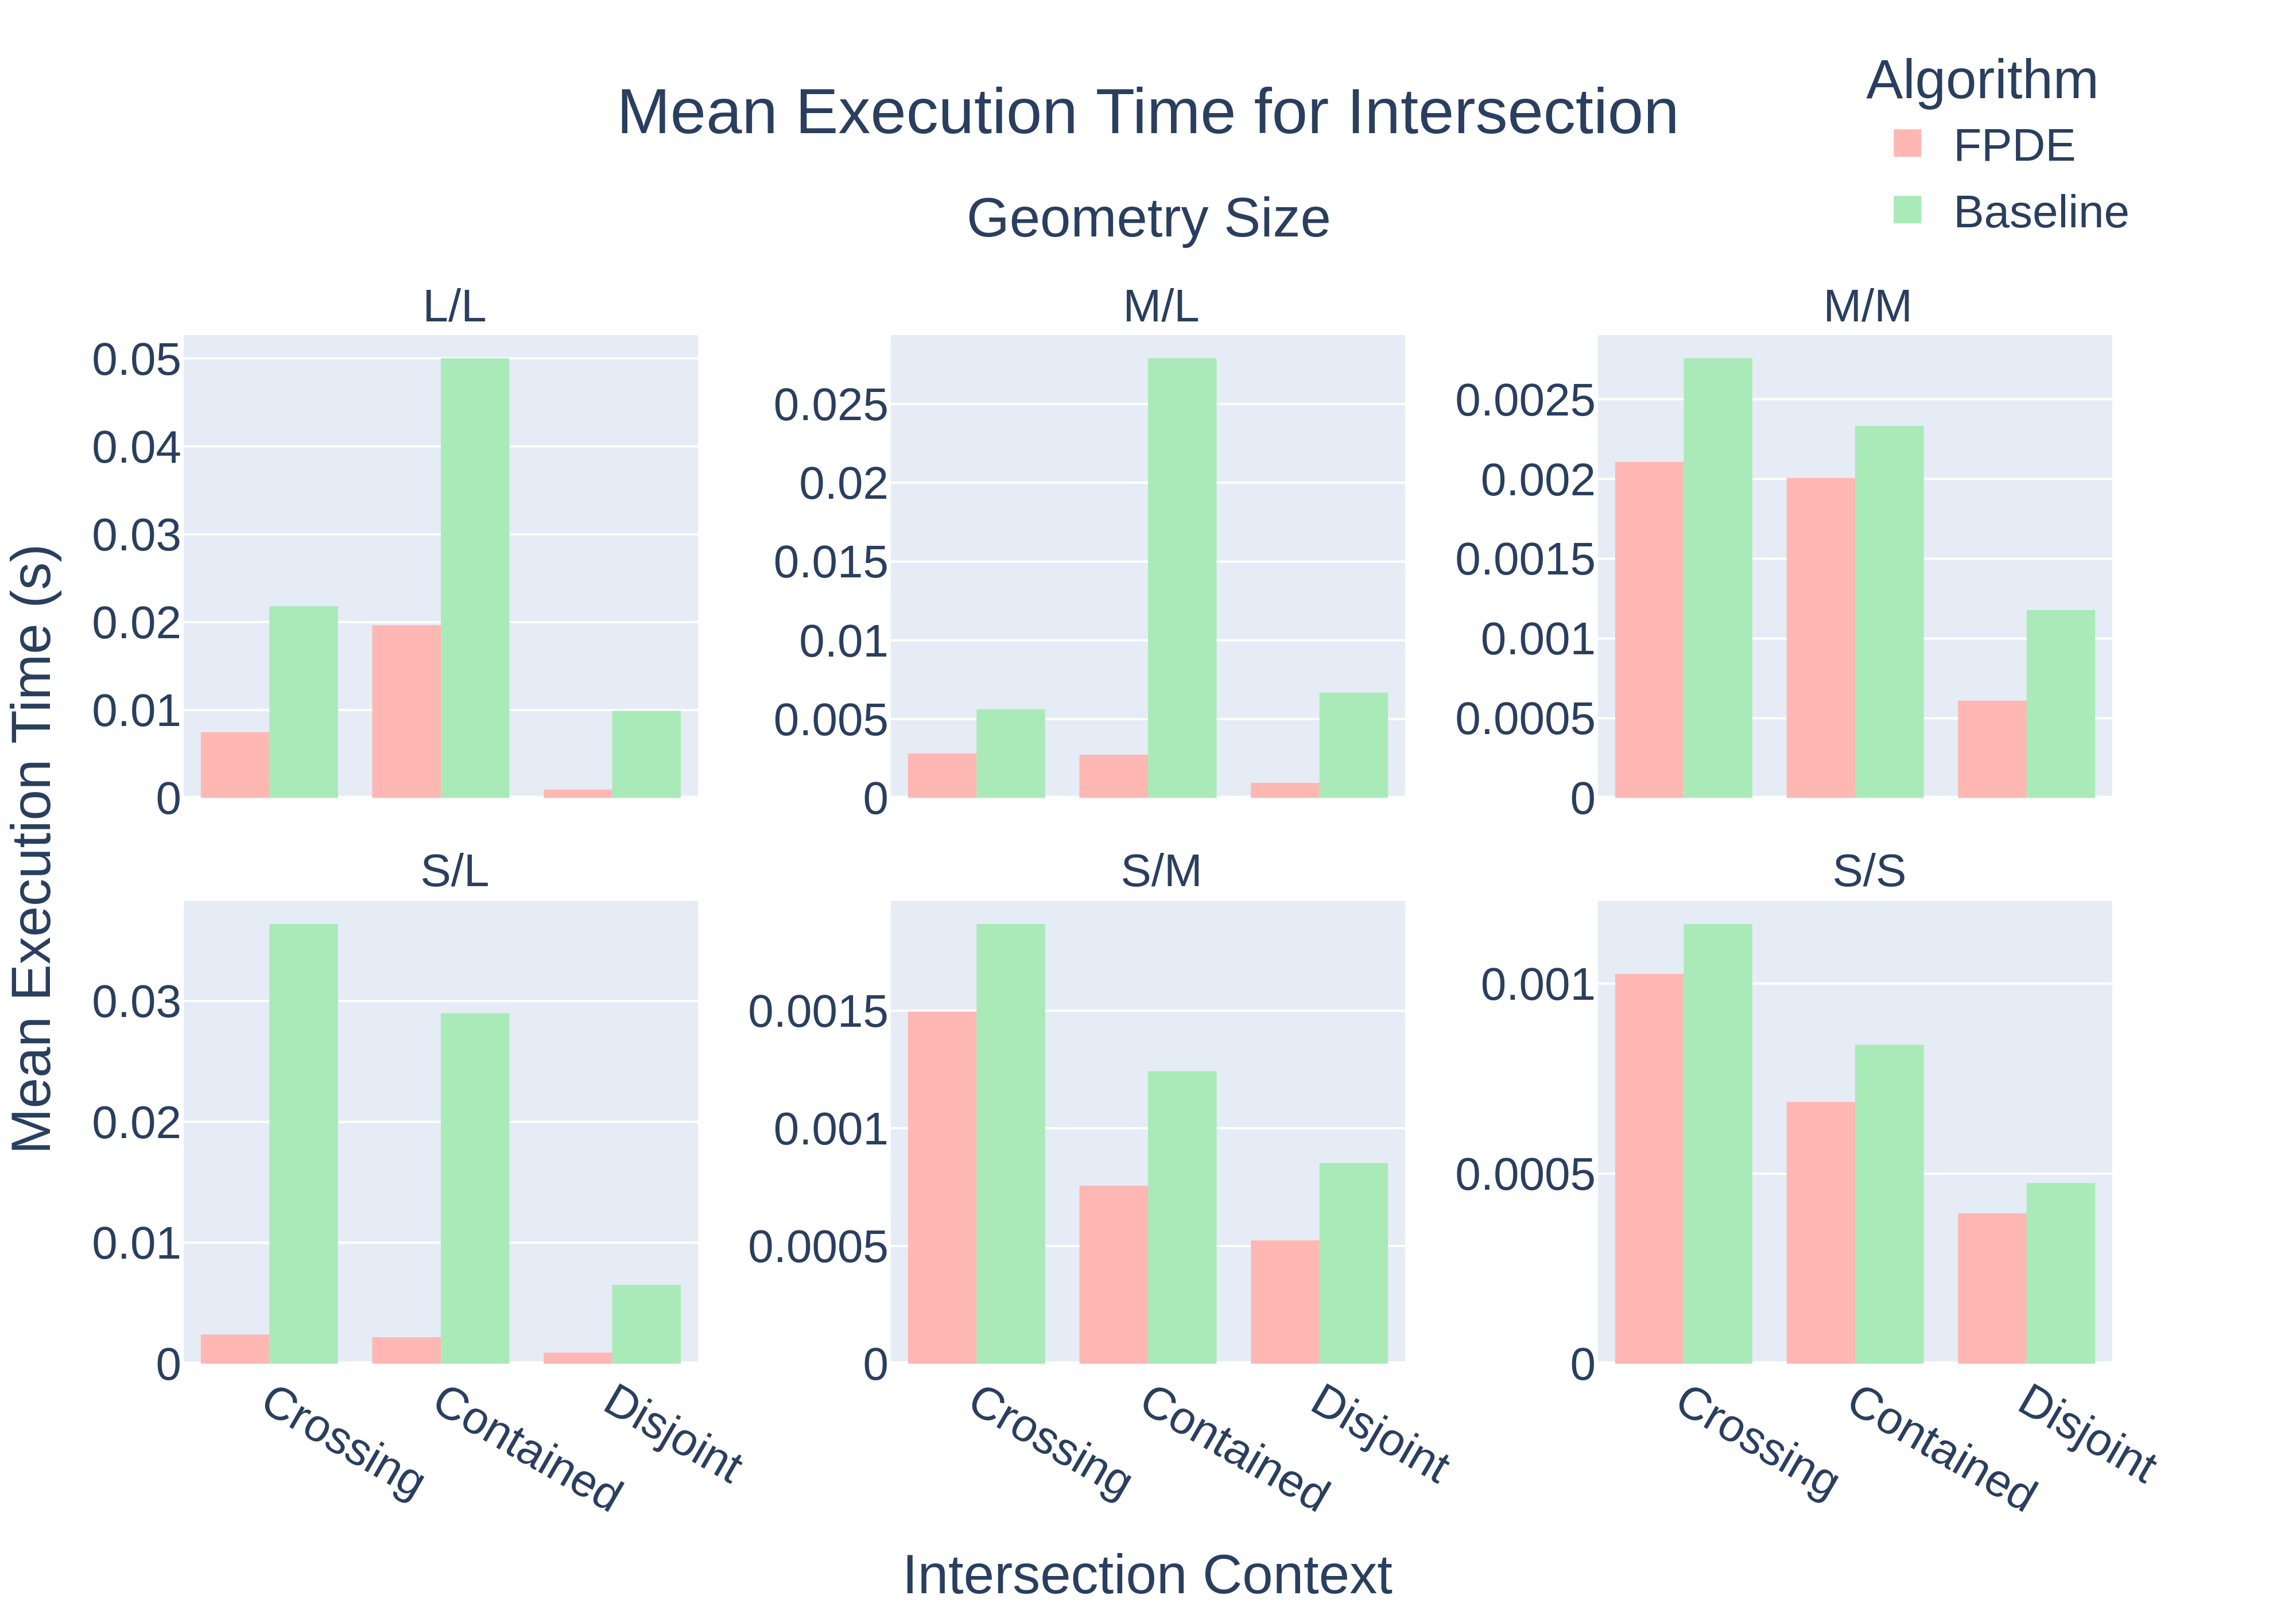
\includegraphics[width=14.5cm]{images/intersection_fpde_vs_baseline.png}

        \caption{Average execution time for FPDE for different contexts and geometry sizes. }
        \label{img:meanIntersection}
\end{figure}

\begin{figure}[htbp]
    \centering
    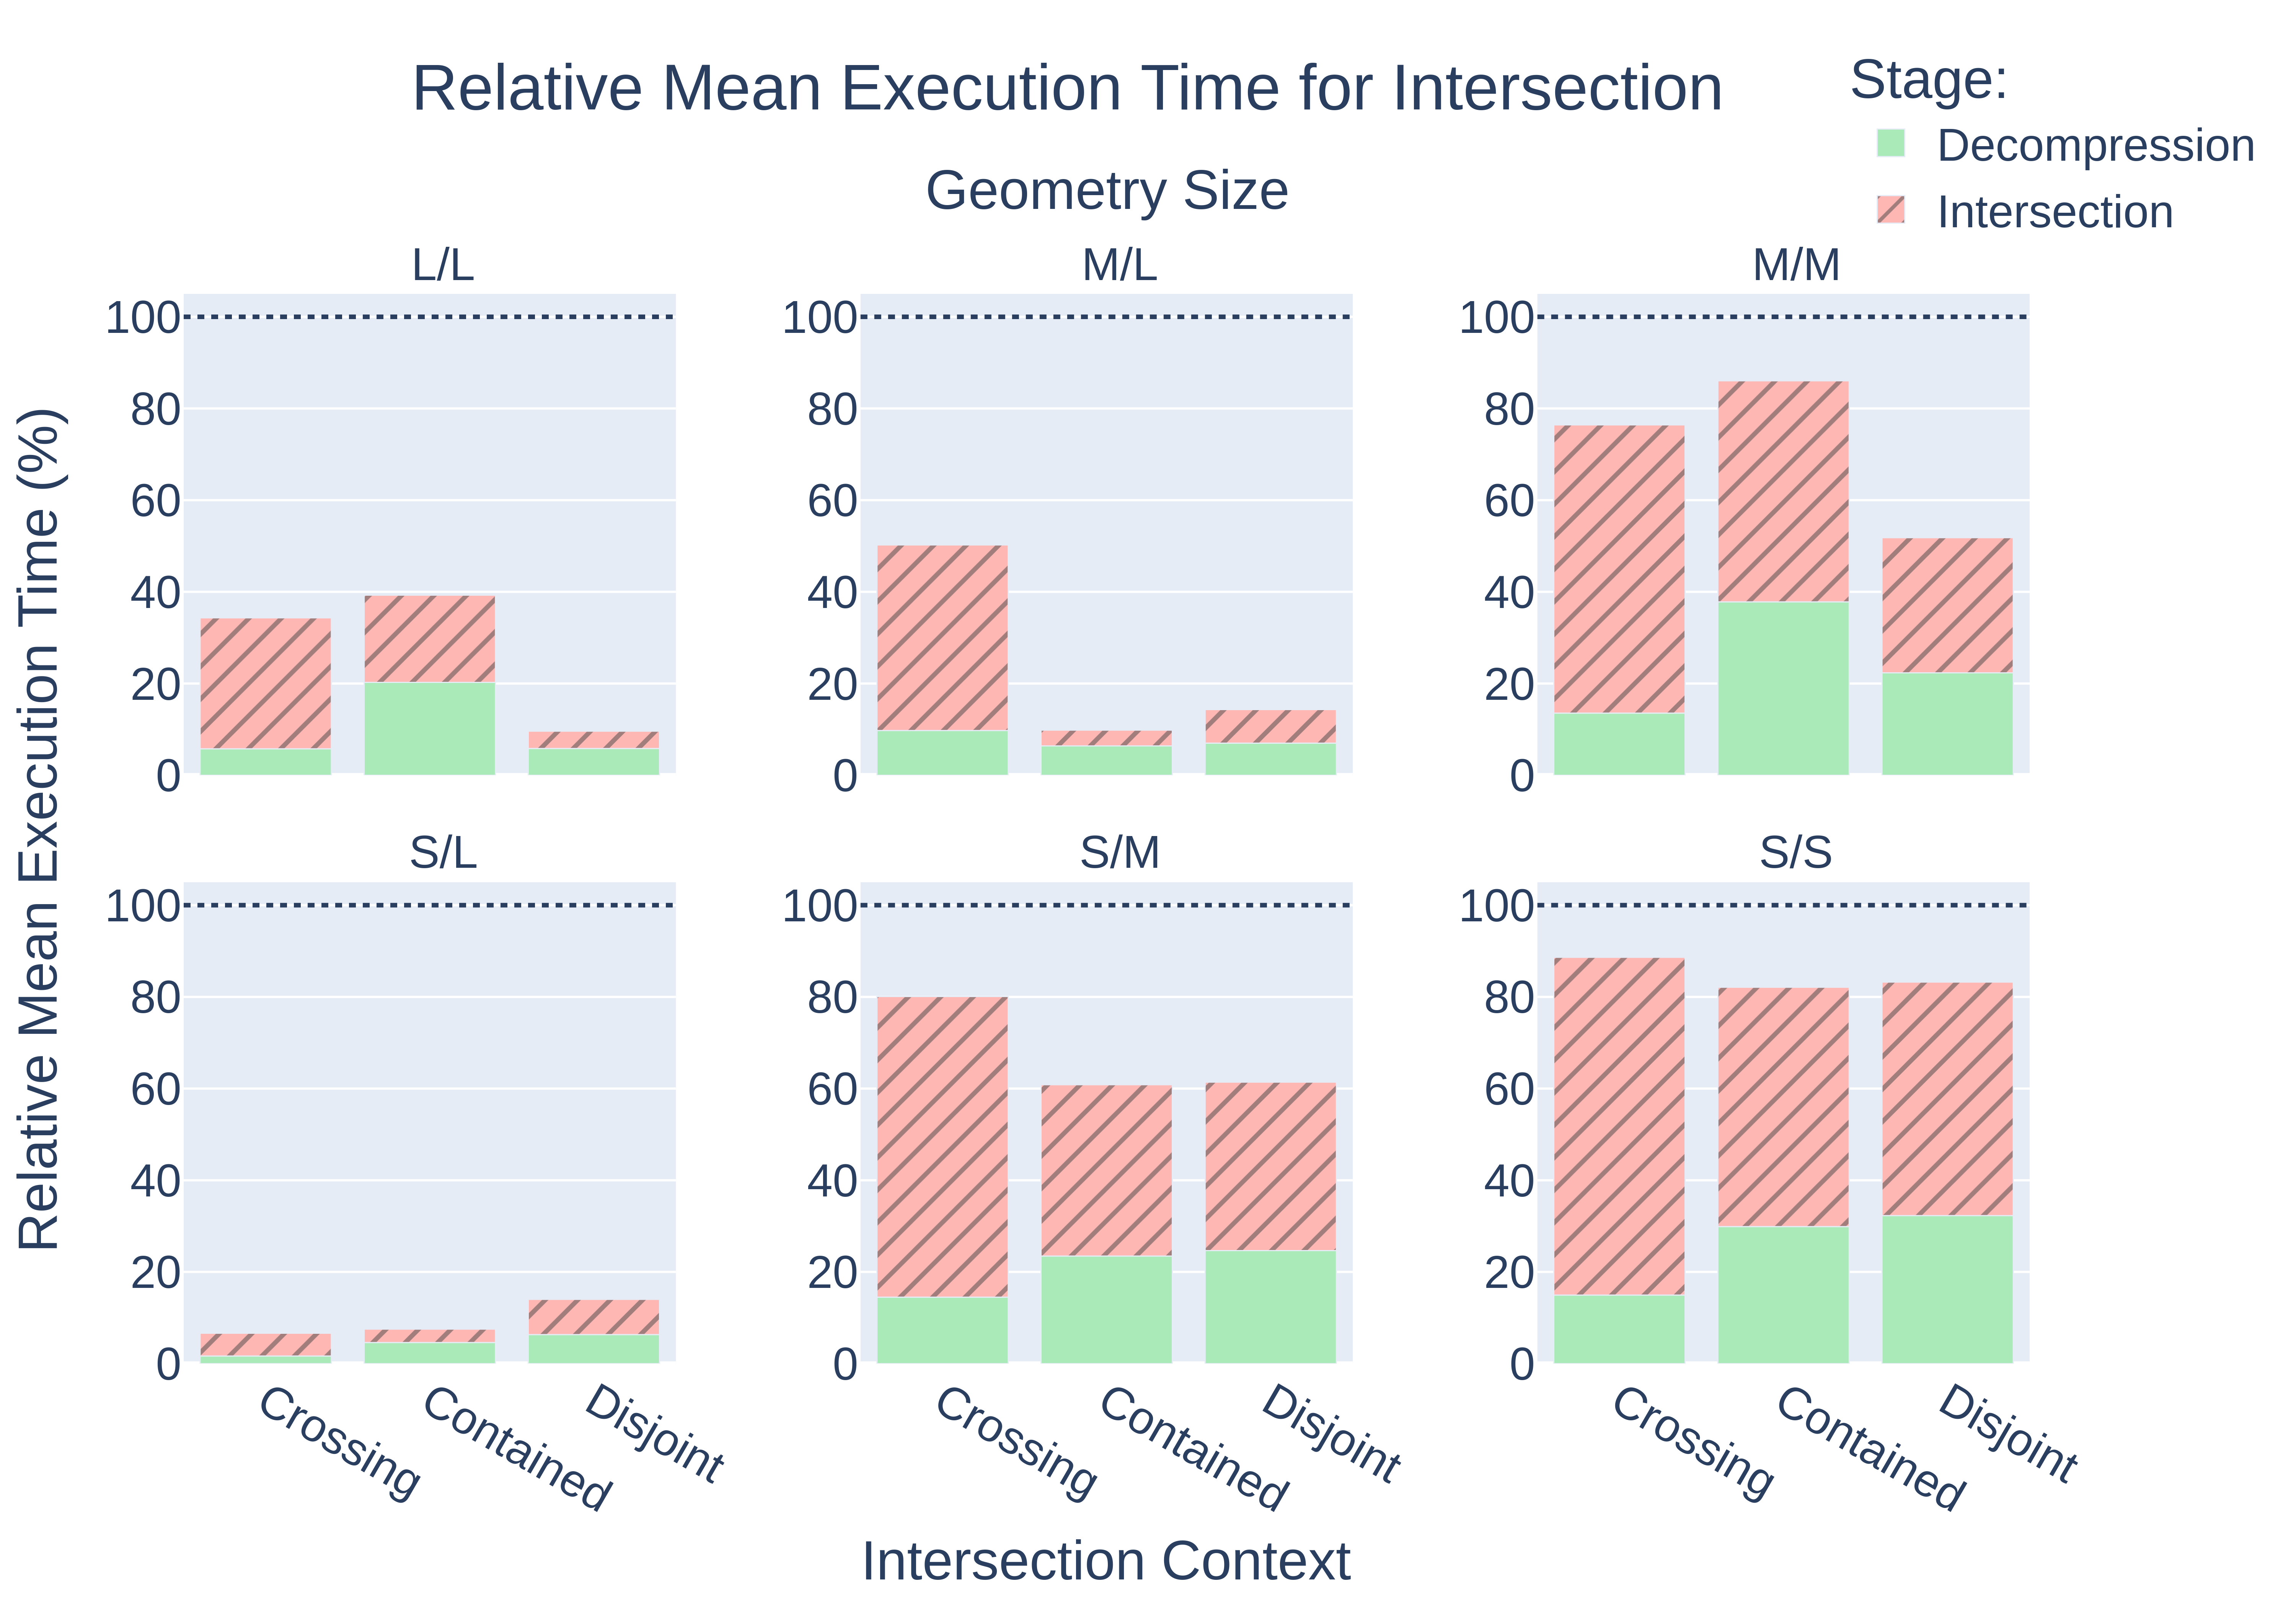
\includegraphics[width=14.5cm]{images/relative_mean_exec_time.png}
    \caption{Fractions for the relative execution time of the decompression and the intersection algorithm stage for FPDE. }
    \label{img:Intersection_exec_time}
\end{figure}

\subsubsection{Number of Vertices in Geometries}
Figure \ref{img:meanIntersection} and \ref{img:Intersection_exec_time} show that the gain of using FPDE for intersection is more significant in scenarios involving complex geometries. This is because complex geometries consist of more chunks, which potentially enables the filtering step in the algorithm to be more fine-grained. In contrast, if a geometry only contains one single chunk, the filtering step has no flexibility in selecting only a subset of the vertices. This reasoning is further supported by Figure \ref{fig:chunks_unfold} showing that on average, calculating the intersection of two simple geometries involves decompressing almost all available chunks, while only a tiny fraction is unfolded for complex geometries.

\begin{figure}[htbp]
    \centering
    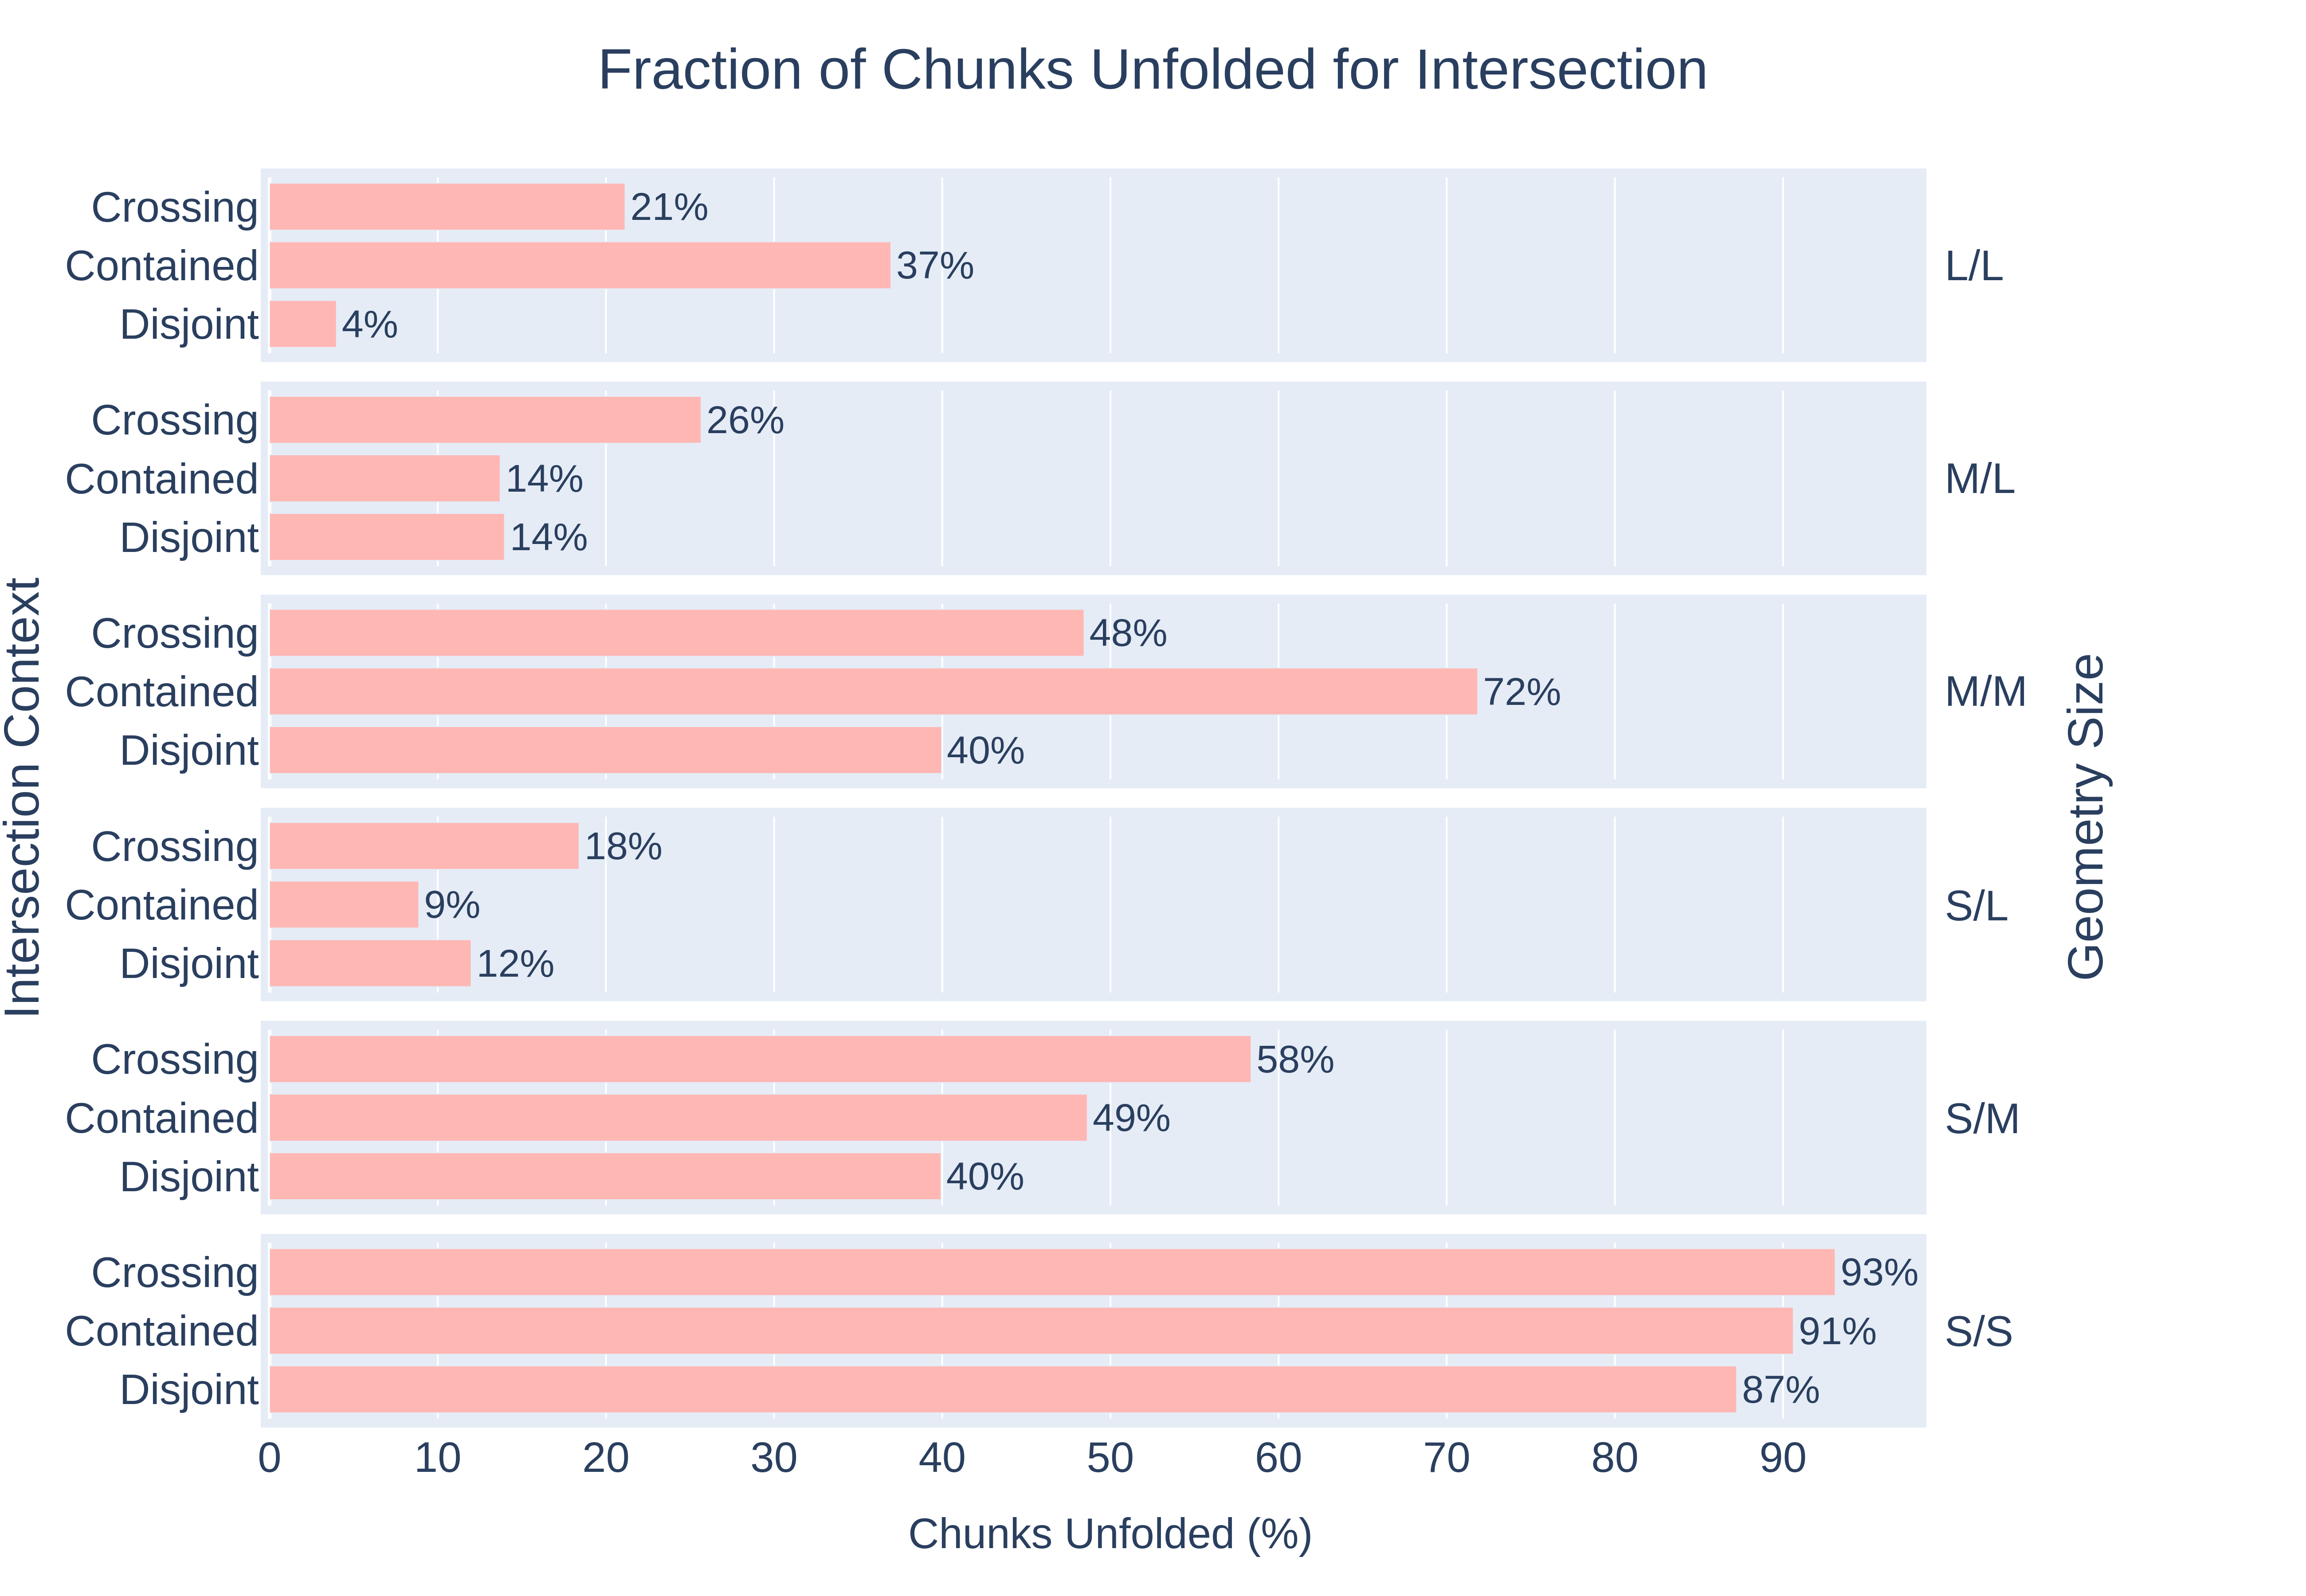
\includegraphics[width=15cm]{images/fraction_of_chunks_unfolded}
    \caption{Fraction of chunks partially decompressed grouped by context and dataset.}
    \label{fig:chunks_unfold}
\end{figure}

\subsubsection{Intersection Context}
The execution time of the intersection operation also depends on the context of the geometries. For example, in the \textit{Contained} case, the performance gain of using FPDE depends on the complexity of the contained geometry. Figure \ref{img:meanIntersection} shows that when a simple or medium-sized geometry is contained within a complex geometry, FPDE significantly outperforms the baseline. This is because FPDE only has to decompress the smaller inner geometry and a tiny fraction of the complex outer geometry, when performing the testing for \emph{contains}, described in Section \ref{sec:pointinshape}.

In contrast, when the geometries' size categories are equal, the relative execution time and the fraction of chunks unfolded are relatively high, as shown in Figure \ref{img:Intersection_exec_time} and \ref{fig:chunks_unfold}. In these circumstances, it is likely that the shapes are tightly arranged, which causes many of the chunk bounding boxes to overlap, resulting in unnecessary decompression for some of the outer geometry's chunks. 

When averaging the relative execution time for FPDE in contexts with two large geometries in Table \ref{tab:partial_decomp_tab}, FPDE achieves an execution time faster by a factor of 3.6 relative to the baseline, which uses full decompression.


\begin{table}[htbp]
\centering
\resizebox{8.5cm}{!}{
\begin{tabular}{|m{2.2cm}|m{1.3cm}|>{\centering\arraybackslash}m{1.8cm}|>{\centering\arraybackslash}m{1.4cm}|>{\centering\arraybackslash}m{1.4cm}|}  % Adjust column widths and center the percentage columns
\hline
\textbf{Context} & \textbf{Size} & \textbf{FPDE RME (\%)} & \textbf{FPDE PD (\%)} & \textbf{Baseline PD (\%)} \\
\hline
Crossing & L/L & 34 & 17 & 36 \\
& M/L & 50 & 19 & 41 \\
& M/M & 76 & 18 & 30 \\
& S/L & 7 & 25 & 52 \\
& S/M & 80 & 18 & 30 \\
& S/S & 89 & 17 & 23 \\
\hline
Contained & L/L & 39 & 52 & 60 \\
& M/L & 10 & 65 & 82 \\
& M/M & 86 & 44 & 54 \\
& S/L & 8 & 61 & 81 \\
& S/M & 61 & 39 & 52 \\
& S/S & 82 & 36 & 42 \\
\hline
Disjoint & L/L & 10 & 61 & 85 \\
& M/L & 14 & 49 & 77 \\
& M/M & 52 & 43 & 66 \\
& S/L & 14 & 45 & 75 \\
& S/M & 61 & 40 & 59 \\
& S/S & 83 & 39 & 48 \\
\hline
\end{tabular}}
\caption{Table with the relative difference of the mean execution time for FPDE in relation to the baseline, along with the percentage of time spent on partial decompression versus the intersection operation for FPDE and the baseline.}
\label{tab:partial_decomp_tab}
\end{table}

\subsubsection{Decompression \& Actual Intersection Operation Relationship}
In Table \ref{tab:partial_decomp_tab}, the relative execution time of FPDE relative to the baseline is presented, together with the corresponding fractions of time dedicated to the decompression or intersection stage. Figure \ref{img:Intersection_exec_time} is a complementary visualization to the table focusing on FPDE. The table shows that the baseline spends more relative time of its execution on decompression in general. Furthermore, it can be inferred that a low relative execution time for FPDE is closely correlated with the proportion of decompression in the total execution. For instance, intersection contexts with low values for the relative mean execution time are coupled with a high ratio of time spent on partial decompression.





\newpage
\label{sec:res_intersection}
\subsection{Intersection: Deltas Size–Time Trade-Off}
\label{sec:chunking}
The variable partitioning into chunks impacts both the compression ratio and the execution time of operations utilizing partial decompression for random access, explained in Section \ref{Random_access}. 
As FPDE has the ability to set a maximum number of deltas allowed per chunk, the partitioning of the chunks can vary depending on the parameter value. 

\begin{figure}[htbp]
    \centering
        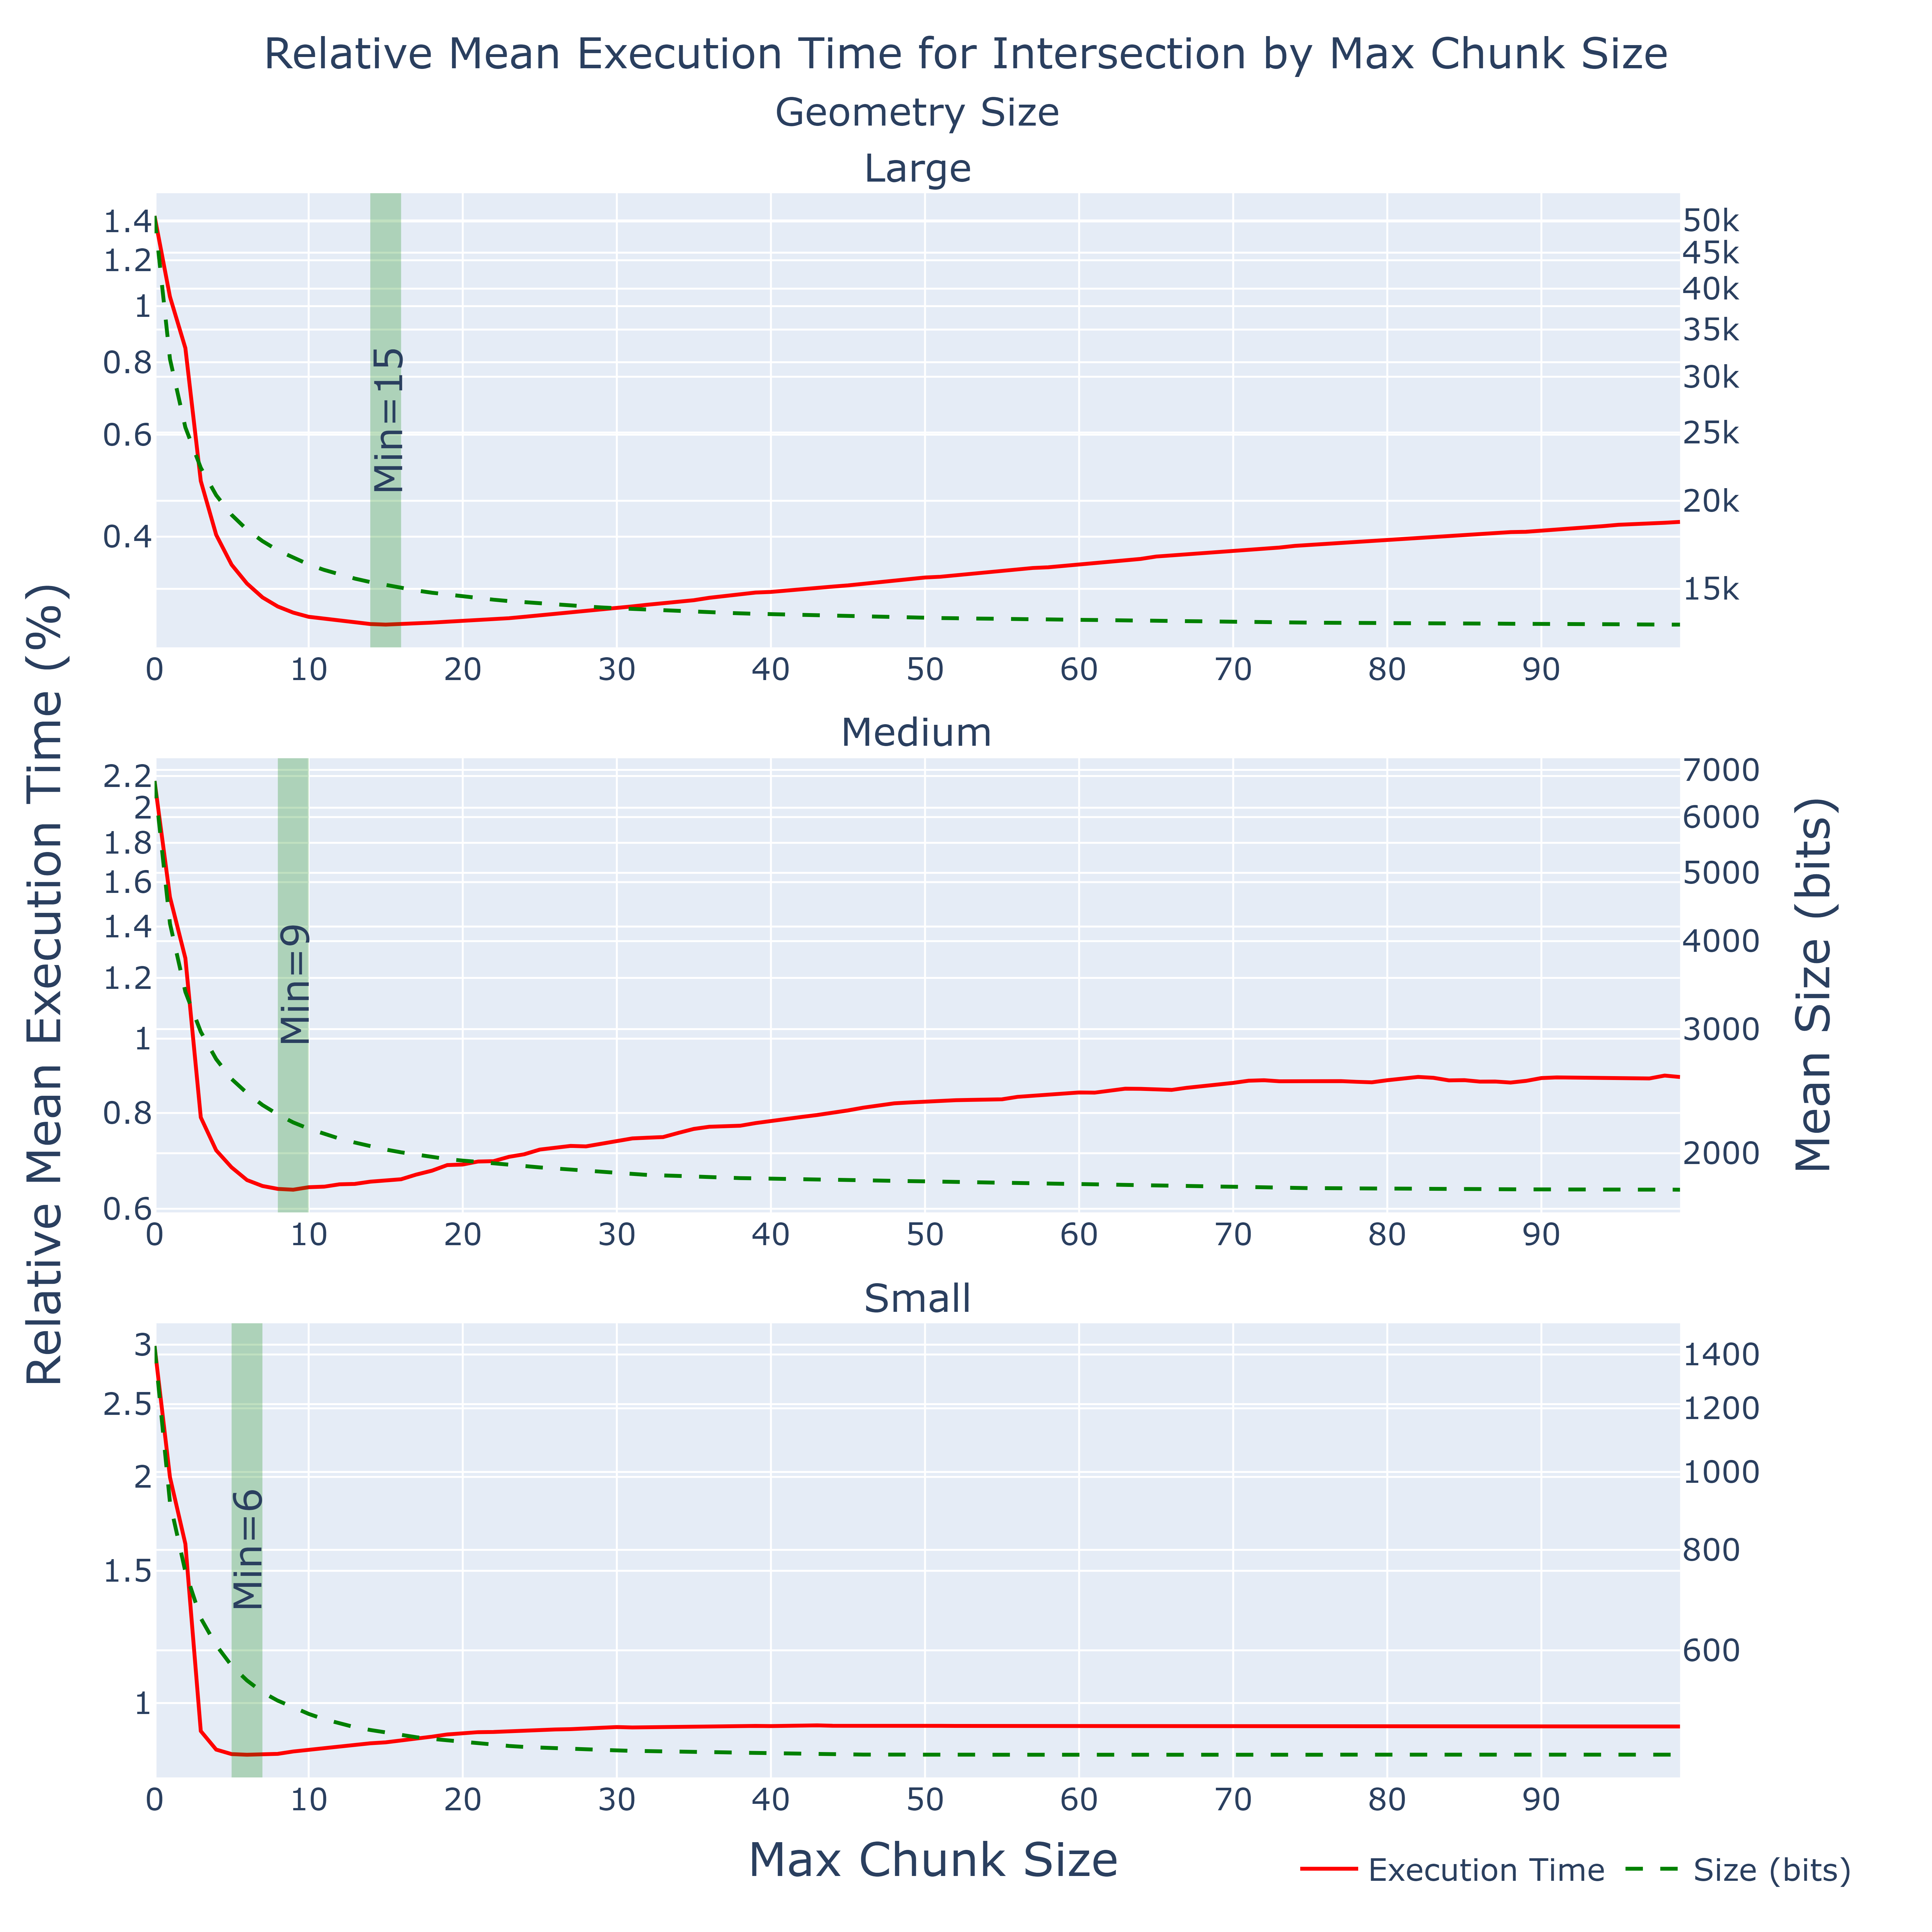
\includegraphics[width=15.5cm]{images/chunk_max_size.png}
    \caption{The left axis (red line) shows the relative mean execution time between FPDE and the baseline with a moving average window of three to compensate for noise, and the left axis (green line) shows the average bit size by the max chunk size parameter.}
    \label{img:delta_max_chunk_perf}
\end{figure}

\subsubsection{Impact on Compression Ratio}
Figure \ref{img:delta_max_chunk_perf} shows how the resulting bit size varies with the maximum chunk size. Increasing the parameter results in a higher average compression factor due to fewer chunk breaks, requiring less coordinates to be represented in full, whereas a small parameter value decreases the compressibility and introduces additional overhead.

The ratio between the number of full coordinates and deltas, if assuming no automatic chunking, can be described with the expression \(r(d) = \frac{1}{d + 1}\), where \(d\) is the maximum number of deltas in a chunk. As the formula and Figure \ref{img:delta_max_chunk_perf} suggests, the ratio decays rapidly, and the effect of the parameter is most significant at lower values.

When setting the parameter to zero and using integrated operability with the default floating-point format, i.e., disabling 32-bit integer decomposed coordinates, the size becomes larger than WKB. This is because setting the value to zero essentially disables delta encoding and introduces additional overhead since each coordinate also includes a chunk header.

On the contrary, when setting an unlimited chunk size, a new chunk is only created when a delta does not fit within the shape's delta bit-length. For homogeneous shapes, the number of chunks is therefore lower since the automatic splitting of the chunks occurs less frequently.

\subsubsection{Impact on Execution Time of Intersection}
As observed in the same figure, the relative mean execution time for intersection also depends on the selection of the maximum number of deltas in each chunk. For intersection queries, the parameter affects two stages, jumping to the correct chunk start and the chunks' decompression time. When increasing the max chunk size, the chunks become fewer and so does the number of jumps required to reach a chunk. On the contrary, when the parameter increases, the chunks also get bigger, and the decompression of each chunk takes longer.

The maximum chunk size also affects the spatial filtering of relevant chunks in the operation. As depicted in Figure \ref{fig:intworld}, intersection queries only extract the relevant chunks through pairwise comparison of the chunks' bounding boxes. For larger chunks, the bounding box will be bigger and, if chunks are too large, irrelevant segments are frequently decompressed due to being in relevant chunks.

In Figure \ref{img:delta_max_chunk_perf}, it also seems that datasets with complex shapes have a slower decay in relative mean execution time with an increased chunk size, compared to datasets with simpler shapes. This is likely due to the fact that complex shapes are able to utilize more chunks, since they have more vertices. The reason for the asymptotic stabilization in execution time when greatly increasing the max chunk size is likely due to deltas overflowing, forcing new chunks even though the chunk max size is not reached.

\subsubsection{Size-Time Trade-Off}
Combining the results above, it is apparent that setting the parameter of maximum chunk size has a large effect on both the size and performance. For the evaluation of the thesis, the value resulting in the highest speed has been chosen. But in a real-world setting, the value can be tweaked to prioritize either size or speed.





% Eventuellt hand picka några fall för att kunna göra djupare analys:
% Strand med ex. en väg som korsar
% Två shapes som är typ helt överlappande


% I bild ovan, mergea datasets, lägg till grå bar (komplement), fixa caps

\section{Entropy Encoding of Deltas}
%Entropy Metrics}
% Huffman, Golomb, Huff Golomb, Huffman Stripped , https://docs.python.org/3/library/bz2.html för burrows wheeler
% Presentera resultat från notebooken, inte huvuddelen av exjobbet så håll kort
For the entropy encoding and analysis of the deltas \textit{32-bit integer decomposed coordinates}, as described in Section \ref{32-bit}, were used to encode the coordinates. All deltas within the datasets presented in Section \ref{sec:datasets} were combined and used for the entropy encoding and evaluation. Note that since the delta values are zigzag encoded integer decomposed coordinates, the values represent the doubled distances between consecutive vertices with alternating signedness. For example, the floating-point decoding of zigzagged values $2$, $3$, and $10000$ is $+ {\color{gray}0.000000}1$, $- {\color{gray}0.000000}1$, and $+ {\color{gray}0.000}5000$.

\begin{figure}[H]
    \centering
    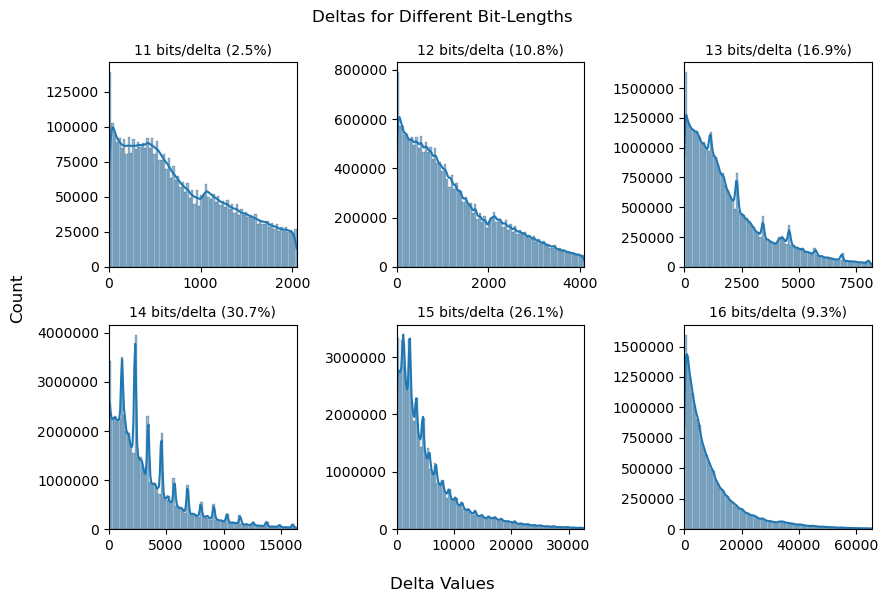
\includegraphics[width=15cm]{images/delta_distrb.png}
    \caption{Frequency distribution of the zigzag encoded delta values interpreted as unsigned integers for the combined datasets. Only the delta bit-lengths accounting for more than 1\% of the combined datasets are visible. 80 bins are used.}
    \label{fig:deltadistrb}
\end{figure}


When analyzing the deltas, it can be concluded that the distribution of values is not uniform. As seen in Figure \ref{fig:deltadistrb}, the values are heavily concentrated around zero, with some spikes in specific values. It is also evident that the decay follows a distribution that closely resembles a geometric distribution, where the slope of the distribution increases for larger delta bit-lengths. According to Figure \ref{fig:deltadistrb}, it seems that the spikes are not present for large delta bit-lengths, but manual analysis concludes that the absence in the graph is instead a result of the binning used when plotting and that the spikes are persistent.

After manually examining the combined frequencies for all bit-lengths, it can be concluded that the most common delta value is 0, followed by $\pm 0.0001145$ and additional seemingly random small values. 0 accounts for 1.5\% and $+ 0.0001145$ for 0.97\% of the values. The spikes then decrease rapidly, where the ten most common values amount to 6\%, and the ten to hundred most common values amount to 8\% of all values.

Zero being the most common value is expected since when a shape only has a change in one axis, i.e., only the x- or y-coordinate is updated, the delta for the other axis becomes zero. Since GIS data is commonly generated by a combination of image processing and manual editing, \emph{snapping} and \emph{procedural generation} of the vertices are likely the causes of the spikes. Snapping can occur in several situations, possibly resulting in vertices with standard spacing; for example, when utilizing tools for simplifying or generalizing shapes. Generation environments can also utilize a grid, where the deltas correspond to distances between the cells. This is further supported by the occurrence of pairwise common values, such as 2290 and 2289, which represent the same magnitude with different signs after zigzag decoding.
\begin{table}[H]
\centering
\caption{Results when applying entropy encoding for all deltas in \emph{Sweden All}, \emph{China Water}, and \emph{Admin Borders}.} 
\begin{tabular}{l|ccc}
\toprule   
 {} & \multicolumn{2}{c}{Compression}\\

Entropy Encoding & Ratio (\%) & Factor & Average Size (bits/delta) \\ 
\midrule
Huffman & \textbf{89.4} & \textbf{1.119} & \textbf{12.59}  \\ 
Sparse Huffman & 89.5 & 1.117 & 12.61  \\
Golomb & 94.5 & 1.058 & 13.32   \\
Golomb + Huffman & 94.4 & 1.059 & 13.30   \\
FpZip & 93.4 & 1.071 & 13.17   \\
\midrule
Global Optimal & 92.1 & 1.086 & 12.98  \\
Per Delta Optimal & \textbf{89.2} & \textbf{1.121} & \textbf{12.56}  \\
None & 100.0 & 1.000 & 14.09  \\ 
\bottomrule
\end{tabular}
\label{tab:entropyDeltas}
\end{table}


As seen in Table \ref{tab:entropyDeltas}, the total size of the deltas can be reduced further by utilizing entropy encoding. The limit induced by Shannon's source coding theorem, i.e., the theoretical value calculated by utilizing Equation \ref{eq:entropy}, corresponds to \emph{Global Optimal} and \emph{Per Delta Optimal} in the table. Per Delta Optimal has one frequency table per delta bit-length, whereas Global Optimal consists of one large table. However, it is important to note that the coordinates of shapes might not be entirely independent of each other, and consequently, the delta values may also exhibit dependence. This violates the assumption of independent and identically distributed symbols in Shannon's source coding theorem, leading to a potential under- or overestimation of the lower bound. Nevertheless, the theorem still provides a reasonable approximation for the lower bound.

The Huffman encodings, both \emph{Huffman} and \emph{Sparse Huffman}, where sparse includes a symbol for representing a missing delta, perform the best. In fact, the Huffman encoding is only 0.2 percent units worse than the lower bound. Golomb encoding, both when coding the quotient using unary encoding and Huffman encoding, reduces the size by around 5\%, as compared to 11\% when only using Huffman encoding. The encoding which utilizes the method proposed in FpZip \cite{fpzip} performs around one percent unit better than Golomb.

Huffman performing better than Golomb is probably a result of the previously discussed spikes, which are deviations from the geometric distribution required by Golomb. The encoding proposed in FpZip is a variant of Golomb encoding and therefore also suffers from an irregular distribution.

Despite this, Golomb encoding or the FpZip variant can be useful when storing the frequency and Huffman table is infeasible. For instance, the possible value range is large when dealing with large delta bit-lengths. Therefore, using \emph{Sparse Huffman} encoding combined with Golomb encoding for missing values is a good way to compress the deltas. With this approach, the Huffman encoding can catch the spikes, while the Golomb encoding approximates the distribution for missing values.






%\section{Predictor Functions}
% Eventuellt kort om predicitior functions accuracy
% \todo{lägg till predictor functions efter redovisning}
\chapter{Discussion}
The following chapter consists of an evaluation when combining the obtained results, followed by a discussion of the generalizability of the datasets, the correctness of the implementation, and future work.
\section{Evaluation of Results}
\subsection{Execution Time Analysis}
As evident by FPDE's performance, compressed data should not be seen as merely disorganized, as there are several opportunities to create structure and optimizations for various purposes. 

The results indicate several advantages of using FPDE in terms of execution time, and, on average, all investigated operations perform better using FPDE compared to the baseline. However, the operation's execution time is highly dependent on contexts such as geometry sizes, intersection type, add vertex index placement, among others. Since FPDE outperforms the baseline in all of these cases, it implies that if the aim is minimal execution time, even though the variability in performance is extensive, it is more beneficial to utilize a scheme like FPDE over conventional compression schemes. 


Nevertheless, increased operability comes at the expense of compressibility. As shown in the results, the size proportions between the induced overhead and the original shape data vary significantly between the datasets, from around 25\% to 63\%, decreasing with the average vertex count of the datasets. Likewise, the relative execution time gains for the operations are higher for complex geometries. However, while simple geometries only experience a speedup of approximately 19\% for intersection when the geometries' bounding boxes overlap, they still achieve an average speedup by a factor of 35.7 when extracting the bounding box. Considering these variations, the balance of the time-space trade-off relies on the geometry size and the type of operation. While the additional overhead for simple geometries might not be worth the tiny gain in execution time for intersection, it may be worth it when getting the bounding box. Alternatively, it can be practicable to toggle the operability support on a per-operation and per-shape basis, allowing the algorithm to utilize partial decompression for situations where the performance gains are most significant and, otherwise, prioritize size and avoid the metadata overhead. It is also worth noting that the overhead induced in the thesis can probably be well reduced in future work, such as by using a quadtree as proposed in Section \ref{sec:quadtreechunk}.


However, some operations do not interfere with time and space trade-offs. \textit{Add Vertex} achieves a similar execution time gain as the bounding box operation, without any additional metadata needed. In this case, the operation is considered a two-way benefit and can thus be used without any trade-off considerations. As a side note, in practice, the partial "re"-compression when adding a vertex is likely very beneficial in GIS editing tools since modifying individual vertices in shapes is a frequent operation.








% i.e., that intersection utilizes the natural forming of chunks in order to perform initial low-resolution filtering using the chunks' bounding-boxes. However, since there is an evident time-space trade-off, adding more operations will lead to a lower compression ratio since more space must be allocated for metadata and other optimizations.



% DONE Overall, as the results show, all operations investigated benefits from partial decompression

% (DONE) It is apparent that compression should not be treated as a black box, since the underlying structure of the algorithms may allow for optimizing of the operations. As evident by FPDE when intersection utilizes the natural forming of chunks in order to perform initial low-resolution filtering using the chunks' bounding-boxes.

% (DONE) There exist several possible optimizations which can be applied to the algorithm used for returning the intersecting shape. For instance, the odd-

% (DONE) Performance of operation and compression depends on the context of geometries 

% (DONE) Decompress and Compress slower than baseline. Operations MUCH faster on average random geoms.

% (DONE) Entropy, adds additional overhead in its conversion 

% (DONE) Fined grained with limit, however performance is changed by this as per graph.

% Different methods of creating chunks, ex. split by quadtree, minimize the overlap between chunks

% Chunks are formed automatically pretty good, but infer maxiumum number of chunks for homogeneous chunks. 

% For Add Vertex the partial "re"-compression is likely greatly benefitically in GIS editing tools, since modifying individual vertices in shapes is likely a common operation.


\subsection{Compressibility Analysis}
\label{sec:compressanalys}
As concluded in the results section, maps data has the potential to be compressed beyond the limits of general-purpose compression algorithms, such as \textit{gzip} and \textit{bzip2}, by exploiting the domain. This section reasons about why the implemented compression scheme performs well and proposes additional ideas, in accordance with the conclusions obtained through the thesis, which may improve the compression further.

Firstly, using arbitrary precision floating-points is probably not needed since a precision higher than a certain decimal digit is likely noise due to the limited accuracy of the data collection methods. By instead quantizing the coordinates to integers, higher compression ratios can be achieved. However, if 64-bit double precision is required, the results indicate that compression by delta encoding the integer representation may still be worthwhile.

\begin{figure}[H]%
    \centering
    \subfloat[\centering Chosen delta bit size per geometry.]{{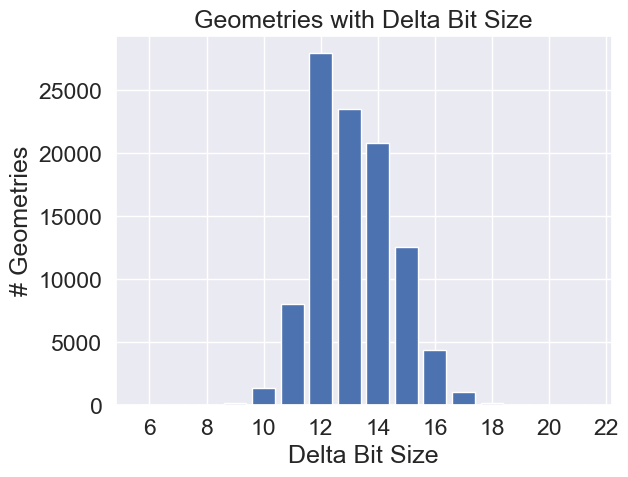
\includegraphics[width=6.9cm]{images/sweden_100000_optimal_delta_size.png} }}%
    \qquad
    \subfloat[\centering Required bit size per delta.]{{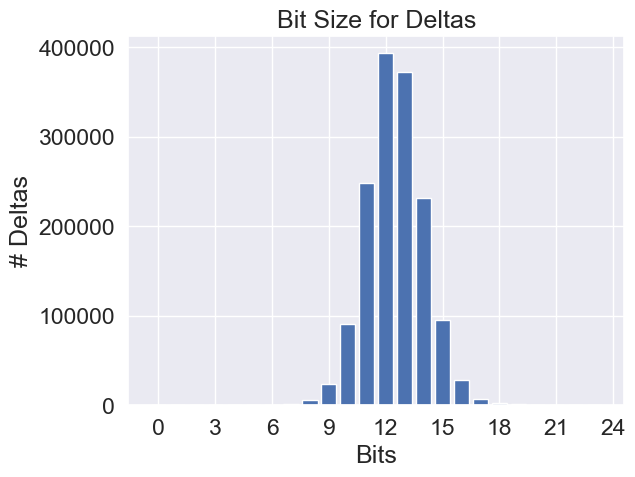
\includegraphics[width=6.9cm]{images/sweden_100000_per_deltas.png} }}%
    \caption{Bit sizes for the deltas and chosen delta bit size in 100 000 random geometries from the \textit{Sweden All} dataset.}%
    \label{fig:swedenbitsize}%
\end{figure}

The delta encoding likely performs well since geometries usually only span a small area of the world, while the integer decomposed coordinates can store distances across the globe.

For map data with seven decimal digits of precision, an accuracy of 1.11 cm is stored, and with each digit removed, it is scaled by a factor of ten. Because maps data is based on several collection methods, with varying precision, it is unlikely that most of the data uses centimeter-level precision and is thus noise in the data. Noise is unsuitable for compression, as it is uniformly distributed and thus no statistical redundancy can be utilized. If those cases can be stripped of the least significant bits containing the noise, entropy coding can be enhanced. One proposition is to infer the precision of the sampling from the data collection method to determine the needed decimal accuracy. Depending on the maps data provider, it might be of interest to perform lossy compression dependent on the geometry size. As seen in Figure \ref{fig:swedenbitsize}, the average delta bit-length for \emph{Sweden All} is 13.2 bits, corresponding to approximately half a meter in real-world measurements. For \emph{Admin Borders}, with a delta bit-length of 20.2 bits or approximately 800 m,  it is unlikely that centimeter-level precision is required, and thus some of the least significant bits can be removed.

With a size of 13.2 bits, a total of 9400 deltas, and the highest precision of $\pm 0.0004700$, longitude/latitude degrees can be represented. Thus, a reduction to 4705 deltas is required to scale down one bit, corresponding to halving the distance in real-world measurements. Here, predictor functions can be used to estimate the deltas and then code the residuals. Since some map structures are very similar, such as buildings and roundabouts, storing the structure as a global model and assigning each shape to a specific model by a constant in the header could likely reduce the size further. 

An interesting observation is that chunks are formed when a delta is large compared to its geometry context, which means that the distances between the chunks are larger than the deltas. This can also affect the execution time, since the chunk bounding boxes get inflated when they span to the next linked chunk. Instead, the linking segments between chunks could be placed in their own bounding boxes.

%An interesting case to examine is when the floating-point exponent bits differ by one when using default FPD encoding, potentially resulting in a significantly larger delta.  To avoid this, the exponent and mantissa could be delta encoded separately.

It may be interesting to investigate whether shapes having an uneven distribution of deltas may result in less compression, such as shapes clustered in certain regions but otherwise sparse. One solution may be to have a variable delta bit-length, where each chunk header contains an extra bit specifying whether a new delta bit-length follows.

Additionally, it is possible to describe the deltas in polar coordinates, where the error of the angle scales with the radius. In this case, the radius is delta encoded as is, while the angle is delta encoded followed by a truncation of decimals, depending on the tolerated error margin. This makes implementing approximation of large distances trivial.







\subsection{Relevance in the Real World}
The thesis has demonstrated that it is possible to reduce the size of maps data from the commonly used WKB to a compressed format by applying quantization, delta encoding, and entropy encoding. If sacrificing compression ratio and embedding metadata, operability support can be added to improve the querying speed of common operations. 

If it is worth sacrificing storage for operability is difficult to decide without more knowledge about the pipeline architecture. If billions of intersection queries are running and I/O is not the bottleneck, then total time can be saved.

However, I/O is commonly the bottleneck in systems, and therefore compressing data to the fullest in order to minimize the I/O use may be preferred \cite{fpzip}. Although, it is worth noting that the overhead induced in the thesis can likely be well reduced and, by adding a toggle-bit for operability integration on a per-shape basis, only one bit is added in comparison to full compression when integrated operability is disabled.


\section{Dataset Properties}
% Why do we see different results?
%more accurate shapes more vertices
For the integration of operations to be beneficial, the benefits should apply to a significant portion of the data. The results show that the improvements increase rapidly with the vertex count, a result of having a higher number of chunks, but simple shapes also benefit from partial compression. However, for simpler shapes, the size of the induced overhead for operability impacts the compression ratio to a greater extent. 

\begin{figure}[H]
    \centering
    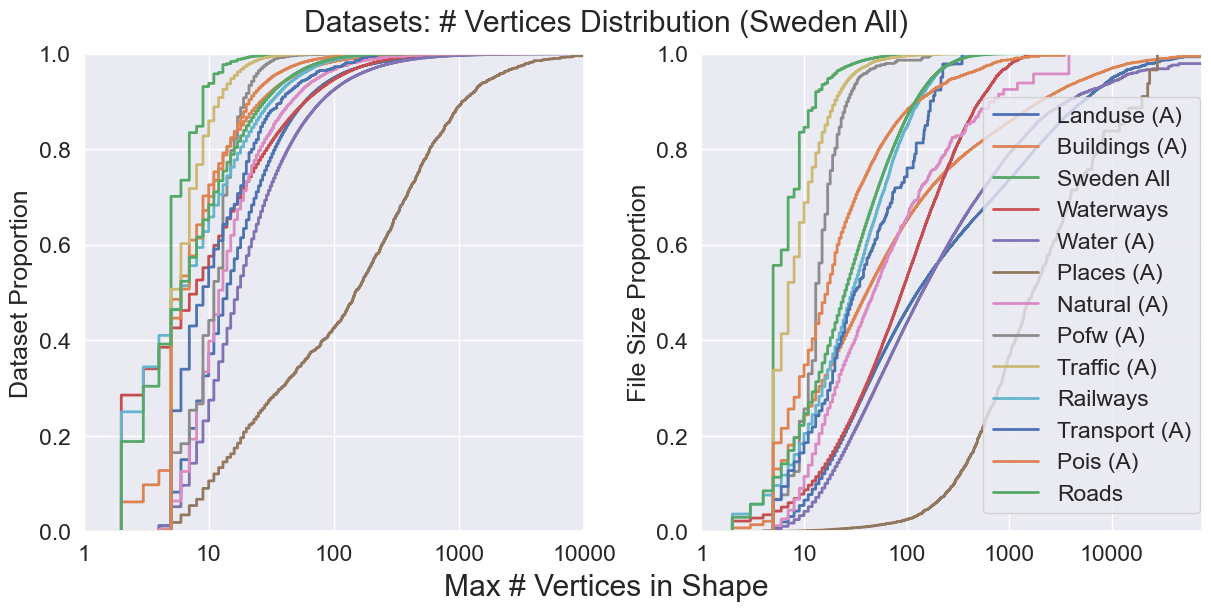
\includegraphics[width=15.15cm]{images/data_distrb_sweden.png}
    \caption{Cumulative distribution of the vertex count for the geometries in \emph{Sweden All}, separated by OSM-tags. The right plot is weighted by the number of vertices, indicating how the overall size is distributed.}
    \label{img:data_distrb_sweden}
\end{figure}

The average vertex count for the geometries in \textit{Sweden All} is 16.4 and 75\% of all shapes have less than ten vertices. Therefore, the percentage of shapes where the gain in execution time significantly outweighs the size overhead is rather low. 

As seen in Figure \ref{img:data_distrb_sweden}, illustrating the distribution of the vertex count for shapes of different types within the dataset, the type of the shape correlates with the average number of vertices. It is logical that geometries covering a large area of the world are constructed using more vertices to increase the detail. Additionally, there are many more houses than country borders, which means that the average is more influenced by simple geometries. Also, complex structures are commonly split into multiple simpler geometries.

The distribution likely also depends on how the spatial data is structured, and our sampling of OSM data might not be a good representation of how other maps services structure their data. For instance, other providers' datasets may consist of many complex geometries due to a higher resolution. It may also be that even though there are fewer geometries in which integrated operability is motivated, the gains are still important. Therefore, it is crucial to obtain precise querying data to identify the exact bottlenecks.

\subsection{Intersection Queries}
% Svårt att hitta faktiskta intersection queries, vi bara approximerar
Due to the high variance in the intersection results, one possible error source is the real-world representativity of the intersection data used in the evaluation. As described in Section \ref{sec:intersectiondataintro}, there are a number of different cases of intersection. The execution time may vary depending on both the intersection case, characteristics of the shapes, and the intersecting region.

Extracting queries representative of real-case use by maps service providers is not trivial. Since intersection queries are commonly used when validating the map, the nature of the queries depends on the validation process and the internal structure of the maps data. A log of recent queries along with the involved geometries would be ideal, but due to secrecy, such data is not publicly available.

It may not be as accurate to construct the intersection queries by picking one geometry at random and finding its neighboring shapes, as done in the thesis, but the queries may still be used as an approximation of real-use scenarios. For example, finding all intersecting geometries and their type is likely frequently used to ensure that no constraints are violated, such as a road intersecting with an ocean.

Additionally, intersection queries tend to involve one complex and one simple geometry for the context \(Contained\). For example, when calculating whether a geometry is within a larger area, such as a state, province, or country, represented by their administrative boundaries. Such queries will benefit significantly from integrated intersection capabilities. This is supported by Table \ref{tab:context_distribution}, showing that the \textit{Contained} case is most common when a complex and a simple geometry is involved.

\begin{table}[H]
\centering
\begin{tabular}{lccc}
\hline
Size & Contained (\%) & Disjoint (\%) & Crossing (\%) \\
\hline
L/L & 0.23 & 2.0 & 11 \\
M/L & 0.13 & 1.5 & 3.1 \\
M/M & 0.08 & 0.66 & 1.4 \\
S/L & 9.9 & 6.9 & 5.2 \\
S/M & 2.9 & 4.5 & 3.7 \\
S/S & 7.6 & 30 & 10 \\
\hline
\end{tabular}

\caption{Context and geometry complexity distribution for the intersection query pairs used in the evaluation.}
\label{tab:context_distribution}
\end{table}

Table \ref{tab:context_distribution} also shows that the distribution of various intersection query types is not uniform, and some accounts for less than 0.1\%. In these situations, it is essential to collect enough data so that even a tiny percentage is a sufficient representation of generality.


The same table shows that some of the intersection query types occur more frequently than others. If a specific query rarely occurs, the results might not have enough support to draw general conclusions. For example, some types of intersection queries are very infrequent for the M/M category, such as \textit{Contained}, which only accounts for $0.08\%$ of the queries.
% \todo{hur många är totalt här? eller skriv hur mycket en procent motsvarar?}



\section{Validity and Correctness}
\subsection{Representativity of Baseline}
Since the implementation is written in Python, which is a mixture of wrappers that execute C code and interpreted Python code, comparing performance and generalizing the results to compile-based languages, including optimizing/JIT compilers, is tricky. When developing the baseline and the extended solution, special care has been taken to ensure that the implementations are as similar as possible in the common parts. Therefore, the results obtained are likely to translate well to speed-optimized languages, but an implementation of FPDE in such a language is required to further verify the results.

Due to the uncertainty regarding performance induced by the language, an alternative language-independent metric of interest is the fraction of unfolded chunks. As discussed in Section \ref{sec:intersection_results}, for the intersection queries used in the thesis, the integrated intersection operation only decompresses around 20\% of the complex geometries. The only way for a baseline implementation to be faster is if the execution time needed for filtering and finding the relevant chunks is larger than the decompression time of the remaining 80\% of chunks. This is unlikely since the operations performed for finding the chunks are rather lightweight. Additionally, irrelevant data can be discarded at an earlier stage, and therefore the intersection algorithm is only performed on a subset of the data. Smaller input is expected to decrease the execution time. Also, when delta encoding is combined with entropy encoding and predictor functions, or other compression techniques, an increase in decompression time is inevitable, and the benefits of partial decompression increase with the decompression time.

\subsection{Implementation Correctness}
Even though FPDE provides a robust solution to a compression format and the specified operations, some cases can lead to unexpected behavior. 

 The intersection algorithm specified in Section \ref{sect:chkintersect} can return the incorrect result if certain types of multipolygons are involved. Suppose a multipolygon, consisting of polygons \(X_1\) and  \(X_2\), intersects with a polygon \(Y\) by \(X_1\) being fully contained in \(Y\), and \(X_2\) being entirely outside it. Additionally, the bounding box of the multipolygon is contained within the bounding box of \(Y\). The correctness of the result in this scenario depends on whether the random point for the ray-sending strategy, outlined in Section \ref{sec:fully_contained}, comes from \(X_1\) or \(X_2\). If sent from the outer one, the ray crosses an even number of edges, and the returning intersection shape will be empty. On the other hand, if the ray is sent from the inner one, the ray will cross an odd number of edges, and it will correctly return \(X_1\). The solution to this inconsistency is to treat \(X_1\) and \(X_2\) as individual entities in the algorithm and return the combined result of each. 
 
 Another case where the intersection algorithm can return incorrect results is with polygons containing inner holes. Suppose a setting where two polygons \(X\) and \(Y\) intersect. \(X\) contains an inner hole \(X_i\), which does not intersect with any of the edges of \(Y\) but is fully contained within the overlapping area of \(X\) and \(Y\). Since the algorithm only constructs the returning shape by traversing the intersection points, the area of the inner hole will incorrectly be excluded from the returning shape. This is solved by decompressing one point in all inner holes with a bounding box overlapping with the returned shape's bounding box and then adding the holes fully inside the returning shape using the ray-sending strategy. 
 
 
 In addition, the algorithm does not support self-intersecting polygons, but as mentioned in Section \ref{sec:intersection}, such geometries are commonly considered errors in spatial data. It is also worth mentioning that the intersection algorithm passes over 99.9\% of all intersection queries from the various datasets in Section \ref{sec:intersection_results}, confirming that these cases of intersection are very rare.


  Furthermore, the formats for representing floating-point coordinates, described in Section \ref{sec:delta_mod}, can result in inaccurate delta values if calculated on coordinates with a longitude degree difference greater than 180. In this case, the floating-point representations cannot fit the delta value, and it will lead to overflow. However, this occurrence is rare in spatial data since it would mean that geometries span half the globe or segments cross the \textit{International Date Line}. For the \textit{variable precision float} format, it can be corrected by extending the exponent section by one bit, and for the \textit{32-bit integer decomposed coordinate} format, by using modular arithmetic on immediate calculations.


\section{Extending Supported Operations}
% How can what we learned be used to further improve other operations?
The operations implemented in the thesis are few compared to the many operations commonly present in geometry libraries. For the format to be adequate for real-case use, it must be possible to implement all operations.


All operations should be able to be implemented following the baseline approach, where the entire geometry is first decompressed, followed by utilizing an existing library function. Accordingly, extending a compression format with more operations can be done iteratively. The ones that bottleneck the system, or are less challenging to implement, could be optimized first, while the non-optimized ones utilize the baseline strategy.

Furthermore, the three implemented operations; \textit{bounding box}, \textit{add vertex}, and \textit{intersection} are characterized by being \textit{constant}, \textit{modifying},
and \textit{binary} operations. Thus, many of the principal components in the implemented operations can be reused to extend the supported operations.
For example, the idea of utilizing the chunks' bounding boxes for intersection can be used to add integrated support for \textit{union}.  Most non-modifying unary operations can be pre-calculated and stored as metadata, and many modifying unary operations can be performed on a per-chunk basis.

\section{Answering the Problem Formulation}
Based on the results and implementation process, the research questions of the thesis can be answered.

\begin{description}
    \item[Q1:] Is it possible to perform operations on compressed geometric data without decompressing the entire geometries?
\end{description}

\noindent Yes, performing operations by partially decompressing geometric data is possible, as evident by the intersection queries only decompressing a fraction of all chunks, and adding a vertex only altering the relevant data sections.
The value of implementing partial decompression depends heavily on the distribution of complex geometries (shapes consisting of many vertices) within the datasets and the performance of the used compression algorithm. The effects are more evident for slower compression algorithms, such as when combining delta and entropy encoding, since the integrated format only unfolds a fraction of the compressed coordinates. 

Additionally, extra overhead is introduced both in terms of extended metadata and the computations needed to determine which data sections to decompress. The number of vertices affects the number of chunks, and with a larger number of chunks, the gains are usually higher since a greater portion of the geometry avoids decompression.

\begin{description}
    \item[Q2:] How can domain-specific constraints and structures, in the context of maps, be exploited to improve the performance of operations and geometry compression?
\end{description}

\noindent Several domain-specific properties can be used to improve the operability and compression performance of maps data, such as representing coordinates as 32-bit integers, delta encoding coordinates, dividing the shapes into mostly non-overlapping chunks, and assuming no self-intersection.

Noise in the data can be reduced by quantizing the coordinates to seven decimals (one centimeter precision) and concatenating the integer and decimal part into a 32-bit integer, resulting in a more compact storage form and higher compression. Delta encoding of map coordinates also performs well, due to individual geometries usually only spanning a fraction of the world. Additionally, simply dividing the shapes into chunks containing a subsequence of all vertices, i.e., a continuous slice of the index vector, results in a division that can be used to improve the performance of operations. Furthermore, by assuming that there are no self-intersecting geometries, any found intersection must be between two separate shapes, reducing the complexity of implementing the intersection operations.  

\newpage
\section{Future Work}
The following section contains explanations of several ideas that can be explored to extend the thesis in future research. Additionally, Section \ref{sec:compressanalys} also presents concepts and motivations for improving the compression ratio further.
\subsection{Implementation in High-Performance Language}
Because the thesis implementation is written in Python, it is not applicable for practical use in a high-performance context. As described earlier, the baseline is also implemented in Python, and thus the results indicate a relative gain and that there exist cases where only a fraction of all chunks need to be decompressed. In order to compete with state-of-the-art geometry compression and further evaluate the potential applications on a large scale, the concepts in the thesis need to be implemented in a high-performance language. Since much of the current implementation is just logic-based and bit-operations, i.e., most of the code for the compression format does not utilize Python libraries, the translation should be straightforward.

\subsection{Further Reducing Interobject Redundancies}
%Kollar bara på enskilda geometrier: sämre kompression
%Spatial parquet column based, kollar på mängd geometrier
It is clear from the results that, in terms of entropy encoding, the deltas are close to the limit calculated using Shannon's source coding theorem when using Huffman encoding. Arithmetic encoding may be able to reduce the size further, by compressing whole chunks rather than individual deltas.  However, the potential additional size reduction is not expected to be groundbreaking.

Therefore, in order to further compress the deltas, which for complex geometries account for the majority of the data, alternative techniques are required. One proposition, when working with maps data, is to differentiate between geometry types. For example, buildings consisting of four vertices are very common, and for such buildings, the deltas should be similar. It would be of interest to examine whether using different probability tables for each geometry type (road/building/water) would result in a distribution that is more skewed and beneficial for entropy encoding. Furthermore, predictor functions based on the geometry type should, for geometries with a standardized structure, be able to reduce the size further.

\subsection{Parallelization of Algorithm}
% Clusters, optimize by partial computation
With the increase of parallel and distributed computing, altering algorithms to enable compatibility with big data environments allows for both horizontal and vertical scaling \cite{parallell}. Vertical scaling utilizes multiple cores or GPUs to divide the workload locally, while horizontal scaling distributes the workload to a number of computers.

In both cases, the workload is divided between workers, and thus it must be possible to decompose the work into non-overlapping parallel tasks. Since FPDE consists of independent chunks, it should be possible to parallelize both the compression, decompression, and some of the operations. For instance, the intersection operation can be divided by assigning each worker to a section of the common bounding box and merging the partial computations.


\subsection{Extended Investigation of Chunking}
While conducting the various performance assessments, it was discovered that the performance of the compression and some of the operations depends on the chunking of the geometries. For instance, Section \ref{sec:chunking} outlines the trade-off between intersection and compression performance when adjusting a parameter that directly influences the chunking of the geometries.

In future work, it would accordingly be of interest to extend the analysis to investigate the more general impact that chunking has on the performance of both the compression and the various operations, as well as how to best decide the values for the parameters that affect it. Similarly, a statistical analysis could be made to examine how various properties of deltas in spatial data can be leveraged to optimize the chunking strategies. For instance, using variable bit-lengths for representing deltas in geometries when there are clusters of deltas with similar magnitudes, but the magnitudes vary between the clusters.

% AddVertex för bounding box, även indicies overflow



% \todo{fixa länkarna i källor}


% Should use consistent formatting when it comes to Names ("FirstName LastName", or "F. LastName")
%\printbibliography
\makebibliography{report}

\begin{appendices}
\chapter{Accessing and Running the Code}
All source code written during the thesis, including the FPDE format, baseline, dataset processing, plotting, and evaluation, is publicly available on GitHub. The repository README contains instructions for setting up the environment and running or extending the implementation.
\\\\
Repository URL: \href{https://github.com/SimonErlandsson/Operable-Maps-Compression}{github.com/SimonErlandsson/Operable-Maps-Compression}.


%\chapter{Popular Science Summary}


% display used packages information unless noflielist is used in the cslthse-msc package option
\printfilelist

%make sure we're on even page with the pop-sci
\checkoddpage
\ifoddpage
\else
   \newpage
   \thispagestyle{empty}
   \mbox{ }
\fi
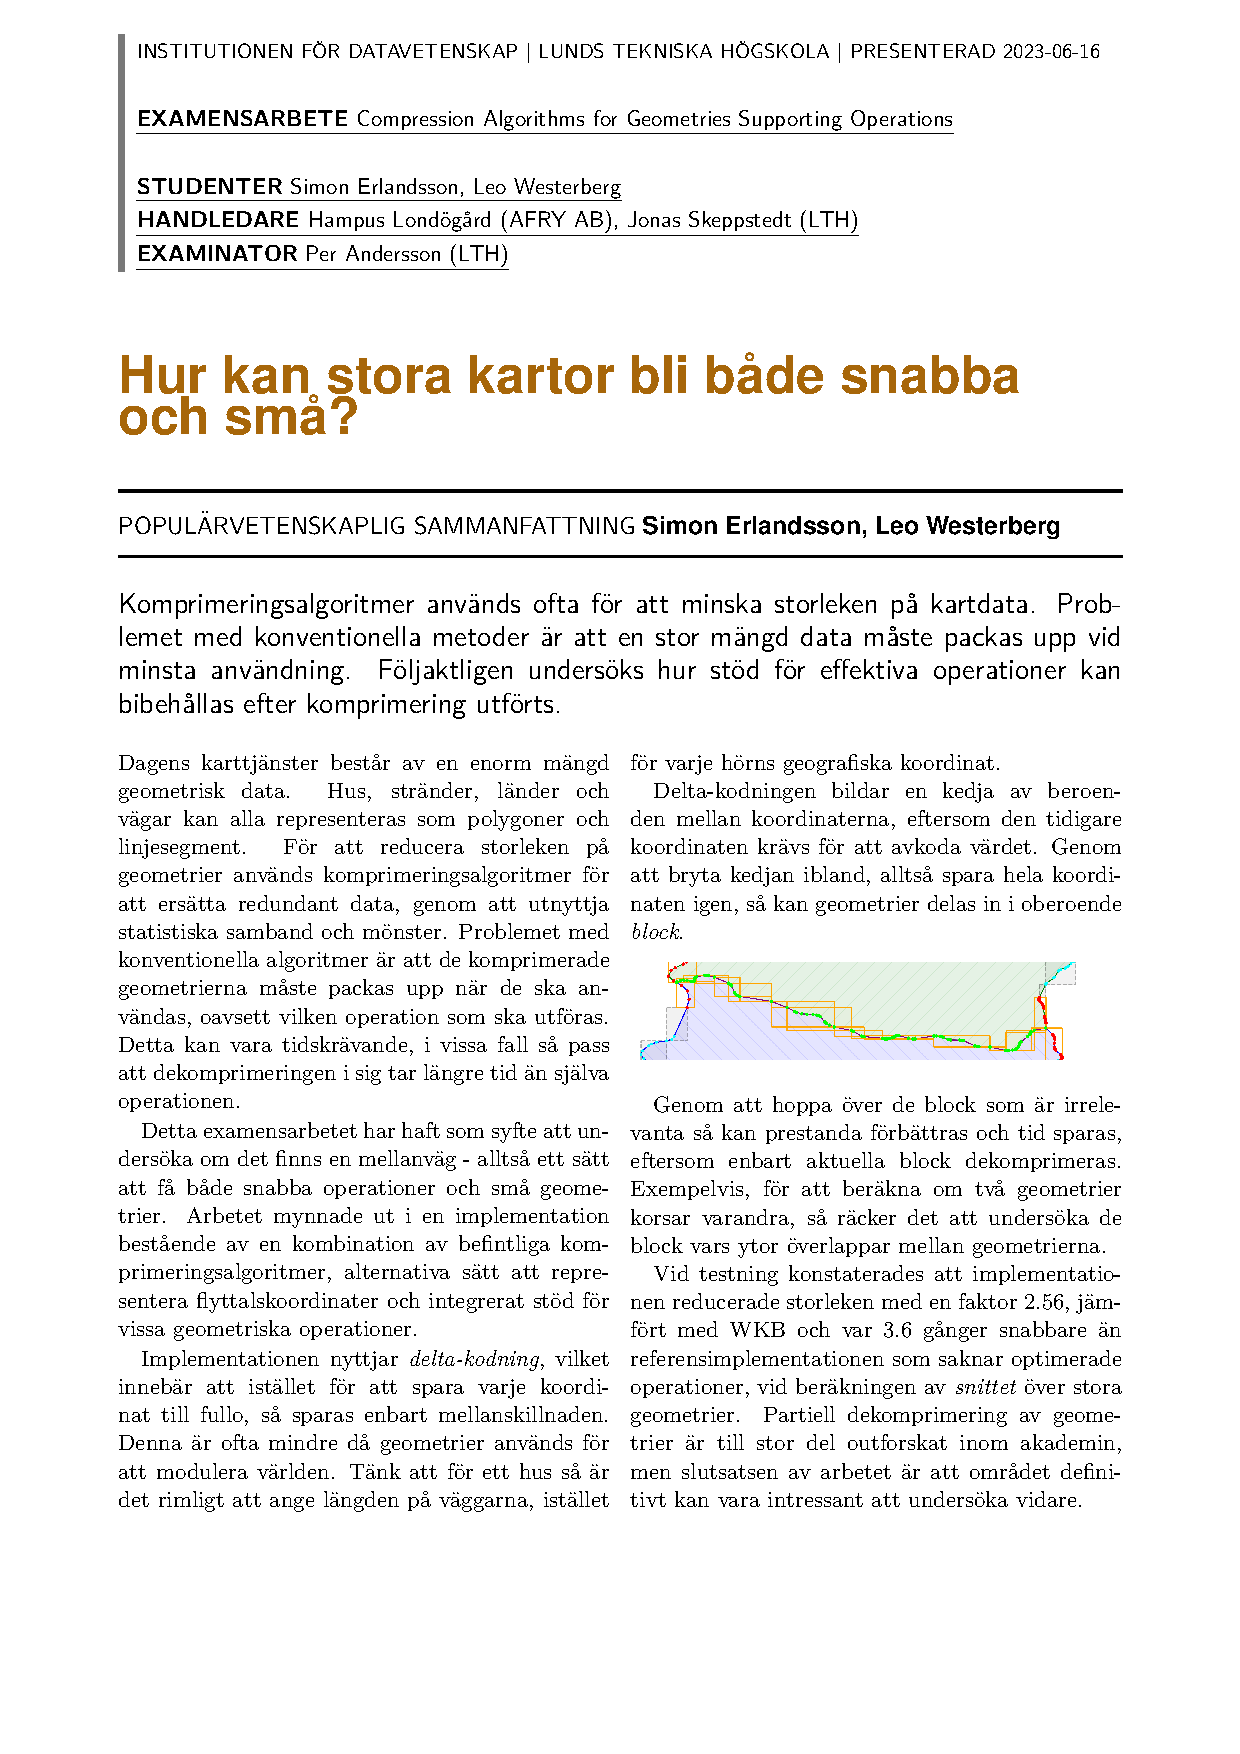
\includepdf[pages={1}]{popsci/popsci.pdf}
\end{appendices}

\end{document}